% ****** Start of file apssamp.tex ******
%
%   This file is part of the APS files in the REVTeX 4 distribution.
%   Version 4.0 of REVTeX, August 2001
%
%   Copyright (c) 2001 The American Physical Society.
%
%   See the REVTeX 4 README file for restrictions and more information.
%
% TeX'ing this file requires that you have AMS-LaTeX 2.0 installed
% as well as the rest of the prerequisites for REVTeX 4.0
%
% See the REVTeX 4 README file
% It also requires running BibTeX. The commands are as follows:
%
%  1)  latex apssamp.tex
%  2)  bibtex apssamp
%  3)  latex apssamp.tex
%  4)  latex apssamp.tex
%
\documentclass[twocolumn,amsmath,amssymb,10pt,groupedaddress,a4paper]{revtex4}
%\documentclass[preprint,showpacs,preprintnumbers,amsmath,amssymb]{revtex4}

% Some other (several out of many) possibilities
%\documentclass[preprint,aps]{revtex4}
%\documentclass[preprint,aps,draft]{revtex4}
%\documentclass[prb]{revtex4}% Physical Review B
%\documentclass[preprint,aps]{revtex4}
%\documentclass[preprint,eqsecnum,aps]{revtex4}
%\documentclass[eqsecnum,aps]{revtex4}
%\tightenlines
%\usepackage[dvips]{graphicx}
%\usepackage{amssymb}
%\usepackage{floatflt}
%\usepackage{array}

%\begin{document}

\usepackage{graphicx}% Include figure files
\usepackage{dcolumn}% Align table columns on decimal point
\usepackage{bm}% bold math
%\usepackage{array}
\usepackage{fancyheadings}
\pagestyle{fancy}
%\usepackage{longtable}
% \usepackage{multirow}
\usepackage[active]{srcltx}
%\usepackage{bibunits}% Separate lists of references
%\usepackage{hyperref}
\bibliographystyle{ieeetr.bst}

%\setlongtables
%\nofiles

\begin{document}

\preprint{Nuclear Data Sheets}
%\draft
\title{EMPIRE-2: the integrated nuclear theory system for evaluating nuclear reactions}


\author{M. Herman, S. F. Mughabghab, P. Oblo\v zinsk\'y and D. Rochman}
\affiliation{National Nuclear Data Center, Brookhaven National Laboratory, Upton~NY~11973-5000}
\author{R. Capote}
\affiliation{Nuclear Data Section, International Atomic Energy Agency, Vienna, Austria}
\author{A. Trkov }
\affiliation{Jozef Stefan Institute, Ljubljana, Slovenia}
\author{M. Sin}
\affiliation{Nuclear Physics Department, Bucharest University, P.O. Box MG-11, Bucharest-Magurele, Romania}
\author{B. Carlson}
\affiliation{ITA/Centro Tecnico Aeroespacial, Sao Jose dos Campos, Brazil}
\author{H. Wienke}
\affiliation{Belgonucleaire, B2480, Dessel, Belgium}
\author{T. Kawano}
\affiliation{T-16, Los Alamos National Laboratory, Los Alamos, NM 87545}
\author{Young-Sik Cho}
\affiliation{Korea Atomic Energy Research Institute, Nuclear Data Evaluation Lab., Daejeon, Korea}

\begin{abstract}

EMPIRE is a modular system of nuclear reaction codes, comprising various
nuclear models, and designed for calculations over a broad range of
energies and incident particles. A projectile can be any nucleon or
Heavy Ion. The energy range starts just above the resonance region,
in the case of a neutron projectile, and extends up to few hundred
MeV for Heavy Ion induced reactions. The code accounts for the major
nuclear reaction mechanisms, such as optical model, Coupled Channels
and DWBA (ECIS03), Multi-step Direct (ORION + TRISTAN), NVWY Multi-step
Compound, exciton model (DEGAS) and the full featured Hauser-Feshbach
model. Heavy Ion fusion cross section can be calculated within the
simplified coupled channels approach (CCFUS). A comprehensive library
of input parameters covers nuclear masses, optical model parameters,
ground state deformations, discrete levels and decay schemes, level
densities, fission barriers (BARFIT), moments of inertia (MOMFIT),
and $\gamma$-ray strength functions. Effects of the dynamic deformation
of a fast rotating nucleus can be taken into account in the calculations.
The results can be converted into the ENDF-6 format using the accompanying
code EMPEND. The package contains the full EXFOR library of experimental
data. Relevant EXFOR entries are automatically retrieved during the
calculations. Plots comparing experimental results with calculations
can be produced using X4TOC4 and PLOTC4 codes linked to the rest of
the system through bash-shell (UNIX) scripts. Publication quality
graphs can be obtained using the powerful and flexible plotting package
ZVView. The graphic user interface, written in Tcl/Tk, provides for
easy operation of the system.

\end{abstract}

\maketitle
\lhead{Nuclear Reaction Evaluation...}
\chead{NUCLEAR DATA SHEETS}
\rhead{M. Herman \textit{et al.}}
\lfoot{}
\rfoot{}
\setlength{\headrulewidth}{0.4pt}
\setlength{\footrulewidth}{0.4pt}

\newpage
\tableofcontents



\newpage
%%%%%%%%%%%%%%%%%%%%%%%%%%%%%%%%%%%%%%%%%%%%%%%%%%%%%%%%%%%%%%%%%%%%%%%%%%%%%%%%%%%%%%%%%%%%%%%%%%%%%%%%%%%%%%%%%%
\section{ToDo and deficiencies}

\begin{itemize}
\item Introduction to be revised
\item CC and DWBA should be updated
\item Fission should be updated
\item Resonance module should be included
\item GUI to be included
\item OMP fitting to be included
\item PCROSS to be expanded
\item gamma-strength functions to be expanded with the new ones
\item Plots (particularly in the resonance section) to be improved
\item Covariances to be written
\item Formatting updated with isomeric cross sections and mixed exclusive/inclusive spectra
\item Resonance section is a bit too long compared to the rest
\end{itemize}

\section{Introduction}
NEED TO BE REVISED !!!

The first version of EMPIRE code was released in 1980. This code originally
contained the Hauser-Feshbach\index{Hauser-Feshbach} theory and the
classical HYBRID\index{HYBRID} model to account for the preequilibrium
effects. The width fluctuation correction was implemented in terms
of the HRTW approach \cite{HRTW,HHM}. Since that time, the code has
been continuously developed. Adding the FKK Multi-step Compound\index{MSC}
mechanism \cite{FKK} lead to the EMPIRE-MSC version. Subsequently,
the NVWY\index{NVWY} formulation of the Multi-step Compound mechanism
\cite{NVWY} was implemented in the HMS-EMPIRE. This version also
included combinatorial calculations of particle-hole level densities.
In addition, a version for Heavy Ion induced reactions (EMPIRE HI)
was developed.

EMPIRE-2 is a totally new release of the code. Contrary to the preceding
developments, which largely consisted in adding new features without
changing the structure of the code, the present version has been rewritten
from scratch, using different programming concepts. Taking advantage
of the relaxed memory limitations, all intermediate files were eliminated,
which together with careful coding of the most crucial parts of the
code, increased the speed of the program by a factor of 20. The new
code is projected to be general and flexible, and can been applied
to the calculation of neutron capture in the keV region, as well as
for Heavy Ion (HI) induced reactions at several hundreds of MeV. All
dimensions in the main code are set up through the parameter statements
contained in the separate file, which is included wherever appropriate,
making any adjustment of the code to the actual problem and/or computer
straightforward. The code has a modular structure. Each module performs
a well defined task and communicates with other modules through a
set of global COMMONS which are included in most of the subroutines.
This assures access to all the resources throughout the code, and
facilitates adding new features and mechanisms.

EMPIRE makes use of several codes, written by different authors, which
 were converted into subroutines and adapted for the present use.
In most cases, the modifications concerned input/output interface
and never affected the physical model contained in the original source.
The following codes are incorporated in the present version of EMPIRE:
\begin{description}
\item [\textbf{ECIS03\index{ECIS}}]Coupled-Channels\index{Coupled-Channels}
and DWBA\index{DWBA} code by J. Raynal~\cite{ECIS},
\item [\textbf{CCFUS\index{CCFUS}}]simplified Coupled-Channels calculation
of HI fusion cross section by C.H. Dasso and S. Landowne~\cite{CCFUS},
\item [\textbf{ORION\index{ORION}~\&~TRISTAN\index{TRISTAN}}]TUL\index{TUL}~\cite{TUL}
approach to Multi-step Direct\index{MSD} by H. Lenske~\cite{ORTRI},
\item [\textbf{DEGAS\index{DEGAS}}]exciton model with angular momentum
conservation and $\gamma$ emission~\cite{Degas} by E. B\v et\' ak
and P. Oblo\v zinsk\' y,
\item [\textbf{DDHMS\index{DDHMS}}]Monte Carlo simulation of the preequilibrium
decay by M.B. Chadwick~\cite{DDHMScode}
\item [\textbf{BARMOM\index{BARMOM}}]fission barriers and moments of inertia
by A. Sierk~\cite{sierk}.
\end{description}
The reader is referred to the original papers for a more detailed
description of these incorporated codes. Furthermore, the package
includes the following stand-alone codes:
\begin{description}
\item [\textbf{EMPEND\index{EMPEND}}]converts EMPIRE results into ENDF-6
format (written by A. Trkov),
\item [\textbf{ENDRES\index{ENDRES}}]merges existing resonance parameters
into ENDF-6 formatted file produced by EMPEND (written by A. Trkov),
\item [\textbf{X4TOC4\index{X4TOC4}}]converts experimental data retrieved
from EXFOR into computational format (written by D.E. Cullen)~\cite{PREPRO},
\item [\textbf{C4SORT\index{C4SORT}}]sorts experimental data in the computational
format file by MAT/MF/MT numbers and incident energy (written by A.Trkov)~\cite{ENDVER},
\item [\textbf{FIXUP\index{FIXUP}}]used to reconstruct MT=4, 103, and
107 (written by D.E. Cullen)~\cite{PREPRO},
\item [\textbf{LEGEND\index{LEGEND}}]calculates linearly interpolable
angular distributions from ENDF data (written by D.E. Cullen)~\cite{PREPRO},
\item [\textbf{LSTTAB\index{LSTTAB}}]tabulates ENDF and EXFOR data in
PLOTTAB format (written by A.Trkov)~\cite{ENDVER},
\item [\textbf{SIXTAB\index{SIXTAB}}]converts ENDF file MF6 to Law 7 representation
(written by A.Trkov)~\cite{ENDVER},
\item [\textbf{PLOTC4\index{PLOTC4}}]plots comparison between EMPIRE results
and EXFOR data (written by D.E. Cullen and A. Trkov)~\cite{ENDVER},
\item [\textbf{CHECKR\index{CHECKR}}]performs format checking of the ENDF-6
formatted file (written by Ch. Dunford)
\item [\textbf{FIZCON}]performs physics check of the ENDF-6 formatted file
(written by Ch. Dunford)
\item [\textbf{PSYCHE}]performs more physics checking of the ENDF-6 formatted
file (written by Ch. Dunford)
\item [\textbf{LINEAR}]converts MF=3 (cross sections) of the ENDF-6 file
into a linear-linear interpolable form (written by D.E. Cullen)~\cite{PREPRO}
\item [\textbf{PLTLST}]prepares list of possible plots by matching experimental
data against ENDF-6 file
\item [\textbf{RECENT}]reconstructs the resonace contribution to the cross
section in linearly interpolable form (written by D.E. Cullen)~\cite{PREPRO}
\item [\textbf{SIGMA1}]Doppler broaden neutron induced cross section (written
by D.E. Cullen)~\cite{PREPRO}
\item [\textbf{STANEF}]Standardizes ENDF-6 formatted file (written by Ch. Dunford)
\item [\textbf{zvvddx}]Produces plots of angular distributions, spectra
and double differential cross sections using ZVView package (written
by V. Zerkin).
\item [\textbf{c4zvd}]ZVView\textbf{\index{ZVView}} plotting package by
V. Zerkin~\cite{ZVView}.
\end{description}
The next chapter outlines nuclear reaction models used in the code.


\section{Thermal Region}
%%%%%%%%%%%%%%%%%%%%%%%%%%%%%%%%%%%%%%%%%%%%%%%%%%%%%%%%%%%%%%%%%%%%%%%%%%%%%%%%%%%%%%%%%%%%%%%%%%%%%%%%%%%%%%%%%

Accurate knowledge of the thermal neutron fission and capture cross sections are of paramount
importance for use as basic standards. Because of this circumstance, considerable experimental
as well as evaluation effort was expended in obtaining very precise and consistent constants at a
neutron energy of 2200 m/sec. The parameters under considerations are the absorption ($\sigma_a$),
fission ($\sigma_f$), and capture ($\sigma_\gamma$) cross sections. These quantities are interrelated
by the following equation:
\begin{equation}
\sigma_a = \sigma_f + \sigma_\gamma
\end{equation}
In addition, when the scattering cross section is known, the absorption cross section can be determined
absolutely  to a high degree of accuracy from a measurement of the total cross section by $\sigma_a=
\sigma_t - \sigma_s$.



%%%%%%%%%%%%%%%%%%%%%%%%%%%%%%%%%%%%%%%%%%%%%%%%%%%%%%%%%%%%%%%%%%%%%%%%%%%%%%%%%%%%%%%%%%%%%%%%%%%%%%%%%%%%%%%%%%
\subsection{Scattering cross section}

The spin-dependent scattering lengths, $a_+$ and $a_-$, associated with spin states $I+1/2$ and $I-1/2$, where $I$ is the spin
of the target  nucleus, can be written as:
\begin{equation}
a_\pm = R' + \sum_{j=1}^N \frac{\lambdabar_j \Gamma_{nj}}{2(E - E_j) - i\Gamma_j}
\label{apm}
\end{equation}
\noindent where $R'$ is the potential scattering length and $\lambdabar$ is De Broglie's wave length divided by $2\pi$. The summation
is carried out over $N$ s-wave resonances with the same spin.

The total coherent scattering length  for non-zero spin target nuclei, is then the sum of the spin-dependent coherent
scattering widths, $a_+$ and $a_-$, weighted by the spin statistical factor, $g_+$ and $g_-$:
\begin{equation}
a = g_+a_+ + g_-a_-  \notag
\end{equation}
\noindent where

\begin{equation}
g_+ = \frac{I+1}{2I+1} \qquad \text{ and } \qquad g_- = \frac{I}{2I+1}
\end{equation}
The coherent, incoherent, and total scattering cross sections can then be expressed in terms of the scattering
lengths by the following relations:
\begin{equation}
\sigma_{coh}=4\pi\left(g_+\cdot a_++ g_-\cdot a_-\right)^2
\end{equation}
\begin{equation}
\sigma_{inc}(\text{spin}) = 4\pi g_+ g_-(a_+-a_-)^2
\end{equation}
\begin{equation}
\sigma_s=4\pi\left(g_+\cdot a_+^2+ g_-\cdot a_-^2 \right)^2
\label{sigs}
\end{equation}



%%%%%%%%%%%%%%%%%%%%%%%%%%%%%%%%%%%%%%%%%%%%%%%%%%%%%%%%%%%%%%%%%%%%%%%%%%%%%%%%%%%%%%%%%%%%%%%%%%%%%%%%%%%%%%%%%%
\subsection{Capture cross section}

The capture cross section, $\sigma_\gamma$, for a single resonance at energy $E_0$, represented by the
Breit-Wigner formalism, is given by:
\begin{equation}
 \sigma_\gamma = \sigma_0 \frac{\Gamma_\gamma}{\Gamma} \left( \frac{E_0}{E} \right) ^{1/2} \frac{1}{1+y^2}
\label{sigmagamma}
\end{equation}
\noindent where

\begin{equation}
y = \frac{2}{\Gamma}(E - E_0)  \notag
\end{equation}


\begin{equation}
 \sigma_0 =\frac{2.608 \times 10^6}{E_0 (\text{eV})} \left( \frac{A+1}{A} \right)^2 \frac{g\Gamma_n}{\Gamma}
\end{equation}

In this relation, $\Gamma_n$, $\Gamma_\gamma$ and $\Gamma$ are the scattering width, the radiative width, and total width
of the resonance, respectively; $\sigma_0$ is the peak total cross section; $A$ is the atomic mass number; $g$ is the
statistical spin weight factor defined below.

If $N$ s-wave resonances of a nucleus are located away from the thermal energy, then their contribution to the thermal
(0.0253~eV) capture cross section is the following expression:
\begin{equation}
\sigma_\gamma^0 = 2.608 \times 10^6 \left( \frac{A+1}{A} \right)^2 \sum_{j=1}^N \frac{g\Gamma_{nj}^0\Gamma_{\gamma j}}{\Gamma_j^2+4(E_n-E_j)^2}
\label{sigmagamma0}
\end{equation}

To calculate the capture cross section, coherent scattering amplitudes, and various spin-dependent scattering cross
sections in terms of neutron-resonance parameters, the above relations, Eq.~(\ref{sigmagamma}) to Eq.~(\ref{sigs}),
were applied~\cite{Mughabghab:06}. If the results of the cross section calculations do not agree with measurements
within the uncertainty limits, then one negative energy (bound) level is invoked or the parameters of the low
energy resonances are adjusted.

%%%%%%%%%%%%%%%%%%%%%%%%%%%%%%%%%%%%%%%%%%%%%%%%%%%%%%%%%%%%%%%%%%%%%%%%%%%%%%%%%%%%%%%%%%%%%%%%%%%%%%%%%%%%%%%%%%
\subsection{Fission cross section}

The fission cross section can be described as a sum over positive and negative energy resonance contributions. In the
framework of the Breit-Wigner formalism, the fission cross section can be obtained from:
\begin{equation}
\sigma_{nf}(E_n) = \frac{2.608 \times 10^6}{(E_n)^{1/2}} \left(\frac{A+1}{A}\right)^2 \sum_j^N \frac{g\Gamma_{nj}^0
\Gamma_{fj}}{\Gamma_j^2+4(E_n-E_j)^2}
\end{equation}

\begin{equation}
\Gamma_j(E) = \Gamma_{nj}(E) + \Gamma_{\gamma j} + \Gamma_{fj} \notag
\end{equation}
%Note that, within the summation sign, $E_n$ at 0.0253~eV cannot be neglected for the fissile isotopes because of the presence of
%negative and/or positive energy resonances near the thermal region.\\
%%%%%%%%%%%%%%%%%%%%%%%%%%%%%%%%%%%%%%%%%%%%%%%%%%%%%%%%%%%%%%%%%%%%%%%%%%%%%%%%%%%%%%%%%%%%%%%%%%%%%%%%%%%%%%%%%%
\subsection{Scattering radius}

The potential scattering length or radius, $R'$, is an important parameter which is required in the calculation of
scattering and total cross section. In analogy with the coherent scattering length, $R'$ is defined by the relation:
\begin{equation}
R' = -\lim_{k \to 0} \left( \frac{Re(\delta'_{OP})}{k} \right)
\end{equation}
\noindent where $Re$ means the real part of and $\delta'_{0P}$ is the optical model s-wave phase shift.
In the optical model, the interaction between the incident particle and the target nucleus
is replaced by a complex potential

%% p 14 eq 32
\begin{equation}
 V(r) = V_0f(r) + iWg(r)
\end{equation}
\noindent where $V_{0}$ and $W$ are the magnitudes of the real and imaginary parts of the optical potential
respectively. The radial dependence of the potentials is specified by the functions $f(r)$ and $g(r)$.
For simplicity, Feshbach, Porter and Weisskopf \cite{Feshbach:54} assumed a spherical square-well potential

%% p 14 no number
\begin{equation}
\begin{aligned}
 f(r) &= g(r) =& 0 \quad \text{for } r > R  \\
 f(r) &= g(r) =& -1 \quad \text{for } r < R   \notag
\end{aligned}
\end{equation}


In the weak coupling approximation, ($W < V_0$) the following expression is derived \cite{Feshbach:54} for $R'$

%% p 15 eq 33
\begin{equation} R' = R \left( 1-\frac{1}{2X_1} \frac{\sin 2X_1}{X_2 \! ^2 + \cos^2 X_1} \right)
\label{rp}
\end{equation}
\noindent where

%% p 15 eq 34
\begin{equation} X = X_1 + iX_2 = \left( k^2 R^2 + \frac{2m}{\hbar^2} (V_0 + iW)R^2 \right)^{1/2}
\label{xeq}
\end{equation}

Note that $R' = R$ when $X_1 = n\pi/2$ where $n$ is an integer In addition, $R'$ has extreme values
whenever $X_1 = n\pi$. Thus, $R'$ modulates around the nuclear radius R.
In contrast, the strong coupling model ($W \ge V_0$) predicts that $R' = R$.

The second term in Eq.~(\ref{rp}) is related to the distant s-wave level contribution, $R^\infty$,
and in R-matrix formalism Eq.~(\ref{rp}) can be written in the simple form for s-waves

%% p 15 eq 35
\begin{equation}
 R' = R(1 - R^\infty)
\label{rpeqr}
\end{equation}
\noindent where

%% p 15 eq 36
\begin{equation}
R^\infty = \sum_n \frac{\gamma_n \! ^2}{E_n - E}
\end{equation}
The summation is carried out over the distant resonances.

\section{Resonance Region}
%%%%%%%%%%%%%%%%%%%%%%%%%%%%%%%%%%%%%%%%%%%%%%%%%%%%%%%%%%%%%%%%%%%%%%%%%%%%%%%%%%%%%%%%%%%%%%%%%%%%%%%%%%%%%%%%%%
\subsection{Resolved Neutron Resonances }

%%%%%%%%%%%%%%%%%%%%%%%%%%%%%%%%%%%%%%%%%%%%%%%%%%%%%%%%%%%%%%%%%%%%%%%%%%%%%%%%%%%%%%%%%%%%%%%%%%%%%%%%%%%%%%%%%%
\subsubsection{Resonance parameters}
The  various considerations which have been taken into account in the assessment
of the resonance parameter data in order to arrive at best values are documented
in~\cite{Mughabghab:06}. In addition to the physics factors, other matters are:
\begin{itemize}
\item  Experimental  energy resolution of the facility.
\item Isotopic enrichment of the sample.
\item Sample thickness.
\item Type of measurements.
\item Method of analysis, whether shape or area analysis was carried out.
\item Normalization procedure for capture, fission and scattering measurements.
\item Uncertainties of the measurements.
\item Assumptions made by the author.
\item Author consistency as determined by comparative studies.
\end{itemize}
 In the present evaluation, the Bayesian approach~\cite{Mughabghab:06,Smith:91} is adopted in this evaluation to
distinguish p-wave from s-wave
resonances for cases where the orbital angular momentum, $l$, have not been determined from measurements. Even though there
is a potential danger of incorrect assignments of $l$~\cite{Garg:81}, the Bayesian approach was used in several cases in
the past. The first investigators to apply Bayes' conditional probability for the determination of parities of $^{238}$U
resonances were Bollinger and Thomas \cite{Bollinger:68}. Subsequently, Perkins and Gyullassy \cite{Perkins:72} and
Oh {\it et al.}~\cite{Oh:00} extensively applied this procedure in the evaluation of resonance parameters.

For a resonance with a neutron width weighted by the spin statistical factor, $g\Gamma_n$, the probability that this resonance
is a p-wave resonance is given according to Bayes' theorem of conditional probability by:
\begin{equation}
P(p|g\Gamma_n)=\left(1+\frac{P(g\Gamma_n|s)\langle D_1\rangle}{P(g\Gamma_n|p)\langle D_0\rangle}\right)^{-1}
\label{bayes}
\end{equation}
\noindent where $\langle D_1\rangle/\langle D_0\rangle$ are the level-spacing ratio, and $P(g\Gamma_n|s)$ (or $P(g\Gamma_n|p)$)  is
the probability that the neutron width is $g\Gamma_n$ if the resonance is an s-wave (or p-wave) resonance.

Eq.~(\ref{bayes}) can be solved by taking into account the Porter and Thomas analysis~\cite{Porter:56} and assuming a (2J+1) law
of level density.

On the basis of an  initial set of resonance parameters, calculations of the
 capture, scattering, fission, and total cross sections are made, as well as
 the coherent scattering amplitude and resonance integrals are made. These
 quantities are compared with the measurements and subsequently adjustments
 are made in the low energy resonance parameters to seek consistency.
 In few cases, one or two negative energy resonances are  invoked to resolve
 the discrepancy.


%%%%%%%%%%%%%%%%%%%%%%%%%%%%%%%%%%%%%%%%%%%%%%%%%%%%%%%%%%%%%%%%%%%%%%%%%%%%%%%%%%%%%%%%%%%%%%%%%%%%%%%%%%%%%%%%%%
\subsubsection{Resonance properties}
From the recommended set of resonance parameretes, Porter-Thomas analysis
 was carried out in order to assign parities to those resonances whose parities
 are not determined experimentally. For a review of these measurements refer
 to~\cite{Mughabghab:06}.
 The reduced neutron widths are distributed according to
\begin{equation}
P(x) = \frac{1}{\sqrt{2\pi x}} e^{-\frac{x}{2}}
\label{px}
\end{equation}
\noindent where
%% p 39 no number
\begin{equation}
x = \Gamma_n^\ell/<\Gamma_n^\ell>   \notag
\end{equation}
This is a special case of a more general distribution called Chi-squared distribution which is represented by

%% p 39 eq 69
\begin{equation}
P(x,\nu) = \frac{\frac{\nu}{2}}{\Gamma \left( \frac{\nu}{2} \right)} \left( \frac{\nu}{2}x \right)^{\left( \frac{\nu}{2} - 1 \right)}e^{-\left( \frac{\nu}{2} \right)x}
\label{pxnu}
\end{equation}
\noindent where $\nu$ is a parameter known in statistics as the number of
degrees of freedom and $\Gamma(\nu/2)$ is the gamma function. One feature of the Chi-squared distributions
is that as $\nu$ increases, the distribution becomes peaked at $x = 1$.

Instead of working with this form of the distribution,  it is much simpler to
analyze the neutron data with the cumulative distibution
\begin{equation}
N(y)= N_o(1-erf(y))
\end{equation}
\noindent where\\
 N(y) = number of levels larger than a prescribed  value of y and
\begin{equation}
 y = \Gamma_n^\ell/2< \Gamma_n^\ell >
\end{equation}
This approach is applied to the resonance parameters of $^{103}$Rh, whose
atomic mass is located near the peak of the p-wave  strength function, {\it i.e.}
its sample population is a mixture of s- and p-wave resonances.
\begin{figure}[htbp]
\scalebox{0.7}{\includegraphics{porter-sp.eps}}
\caption{Porter Thomas distribution for all observed resonances of $^{103}$Rh.}
\label{rh103pt}
\end{figure}
\begin{figure}[htbp]
\scalebox{0.7}{\includegraphics{porter-s.eps}}
\caption{Porter Thomas distribution for s-wave resonances of $^{103}$Rh assigned on the basis of Bayesian analysis.}
\label{rh103s}
\end{figure}

In Fig.~\ref{rh103pt}, where all resonances are assumed as s-wave, note that
there is an excess of weak resonances, and it is not possible to fit the data
with a single PT distribution. On the other hand, in Fig.~\ref{rh103s}, the s-wave resonances
are assigned on either  measurements and/or  Bayesian analysis, a good fit
obtained for a threshold value of 0.2~meV below which about 30 weak s-wave
resonances missed detection. Similarly, the p-wave resonances are well described
by a PT distribution (Fig.~\ref{rh103p}).
\begin{figure}[htbp]
\scalebox{0.7}{\includegraphics{porter-p.eps}}
\caption{Porter Thomas distribution for p-wave resonances of $^{103}$Rh assigned on the basis of Bayesian analysis.}
\label{rh103p}
\end{figure}

Dyson and Mehta \cite{dyson:63} introduced a statistics ($\Delta_3$) which describes long range correlations and is defined as the mean square deviation of a staircase plot (cumulative number of resonances versus
energy) from a best fit straight line. That is,
%% p 37 eq 62
\begin{equation}   \Delta_3 = \min_{A,B} \left[ \frac{1}{\Delta E} \int_0^{\Delta E} (N(E) - AE - B)^2 dE \right]
\label{delta3}
\end{equation}
\noindent where $y = AE + B$ represents the fit corresponding to the minimum value of $\Delta_3$.  Dyson and Mehta \cite{dyson:63} derived the average value
and standard deviation (S.D.) of  $\Delta_3$.   The results are
%% p 34 eq 63
\begin{equation}
\begin{aligned}
<\Delta_3> &= \frac{1}{\pi^2} (\ln N - 0.0687)  \\
 \text{S. D.}&= 0.11
\label{delta33}
\end{aligned}
\end{equation}

The $\Delta_3$ statistics was used extensively by the Columbia group~\cite{liou:72} as a sensitive test for the detection of spurious levels (resonances due to impurities or due to p-wave neutrons) or non-observation of weak resonances. Departure of the experimental $\Delta_3$ value as determined by Eq.~\ref{delta3} from the theoretical value gives an indication of these problems.

The $\Delta_3$ statistics of Dyson and Mehta~\cite{dyson:63} can be applied to resonance data of nuclei  with zero target spin  to determine the quality of the data as to whether resonances missed experimental detection and/or p-wave resonances are included in the sample population. This procedure is applied to the resonance data of  $^{166}$Er  where Bayesian analysis shows that the weak resonances at 110.63, 1545.6, 1678.9, and 2699.6~eV are possibly  due to p-wave neutron interaction, based on  p-wave  strength function values of 0.7 or 1.0 in units of 10$^{-4}$  (Table~\ref{bayesian1}).

A staircase plot of the number of resonances as a function of neutron energy indicates that resonances do not seem to have been missed up to neutron energy of 4.2~keV (Fig.~\ref{er166}). Furthermore, a Porter-Thomas distribution analysis  yields an average s-wave level spacing, $D_0=38.4 \pm 2.5$~eV, in the energy region below 3~keV. $\Delta_3$ statistic are carried out for several cases and the results are summarized in Table~\ref{bayesian2}. Also,the values of the s-wave average level spacing obtained from the least squares fit to the staircase diagram is for the three cases.

In case A resonances at  110.63, 1545.6, 1678.9, and 2669.6~eV are assumed as p-wave; in case B, the p-wave resonances assumed are 110.63, 1678.9, and 2669~eV, while in case of the p-wave resonances are 110.63 and 2669.6~eV. Note that the experimental $\Delta_3$  for the three cases are in agreement with theoretical values within the standard deviation (see Eq.~\ref{delta33}). However, case C is favored on the basis of additional information obtained from PT analysis which yields a s-wave level spacing  of 38.0$\pm$1.8~eV~\cite{Mughabghab:06}.

\begin{table}[htbp]
\caption{Bayesian analysis of some weak $^{166}$Er  resonances. The calculations
are based on $S_0=1.8$ and $S_1=0.7$ or 1.0 in units of 10$^{-4}$. }
\label{bayesian1}
\begin{center}
\begin{tabular}{lcc}
\hline
Resonance Energy &  p-wave probability&     p-wave probability\\
(eV)             &     ($S_1=0.7$)    &           ($S_1=1.0$)\\
\hline
110.63           &     0.85           &      0.94\\
1545.6           &     0.69           &      0.84\\
1678.9           &     0.53           &      0.77\\
2669.6           &     0.81           &      0.89\\
\hline
\end{tabular}
\end{center}
\end{table}

\begin{table}[htbp]
\caption{Application of the Dyson-Mehta $\Delta_3$ statistics  to $^{166}$Er resonances
   below  4.2~keV. See text for details. }
\label{bayesian2}
\begin{center}
\begin{tabular}{lllr}
\hline
Case No  & $D_0$ (eV)&      $\Delta_3$ (Exp.) &     $\Delta_{DM}$\\
\hline
A     &    39.9   &   0.53   &      0.47 $\pm$ 0.11\\
B      &   39.4   &   0.40   &      0.47  $\pm$ 0.11\\
C       &  38.3   &   0.45   &      0.47  $\pm$ 0.11\\
\hline
\end{tabular}
\end{center}
\end{table}

\begin{figure}[htbp]
\scalebox{0.9}{\includegraphics{er166.eps}}
\caption{Stair case plot for $^{166}$Er up to 4.2~keV.}
\label{er166}
\end{figure}

%%%%%%%%%%%%%%%%%%%%%%%%%%%%%%%%%%%%%%%%%%%%%%%%%%%%%%%%%%%%%%%%%%%%%%%%%%%%%%%%%%%%%%%%%%%%%%%%%%%%%%%%%%%%%%%%%%
\subsection{Unresolved Neutron Resonances}
%%%%%%%%%%%%%%%%%%%%%%%%%%%%%%%%%%%%%%%%%%%%%%%%%%%%%%%%%%%%%%%%%%%%%%%%%%%%%%%%%%%%%%%%%%%%%%%%%%%%%%%%%%%%%%%%%%
\subsubsection{Background}
Because of the availability of extensive and  highly accurate capture measurements in the unresolved energy region (URR) with uncertainties of  the order 3-4~\%, these specific data can serve as testing ground for the validation of the average resonance parameters obtained from  the resolved energy region~\cite{Mughabghab:06}. We note specifically  that Bayesian analysis was extensively applied previouly at BNL~\cite{Mughabghab:06,Oh:00} in order to distinquish between s- and p-wave resonances on the basis of the the "strength" of resonances. However, this approach can lead to ambiguities in the determination  of  average spacing of neutron resonances, as well as   average radiative widths, and  neutron strength functions, for the various partial waves. As an illustration, when Bayesian analysis is applied  to the strong $^{98}$Mo at 429, 612, and 818 eV, the result  shows that these are s-wave resonances, when in reality they were experimentally established~\cite{Mughabghab:71} as p-wave in character. This is due to the overlap of the weak s-wave and the strong p-wave resonances whose respective reduced neutron widths are governed by Porter-Thomas distributions.

Another problem which  can complicate the analysis in the resolved energy region, arises because of  prevalent experimental  factors, such as neutron energy resolution, Doppler broadening, and  the difficulty of detecting weak resonances, especially in total cross section measurements. In view of these considerations, the analysis of accurate capture cross sections in URR can shed additional light on the average parameters and hence resolve these inherent problems.

\subsubsection{Theoretical considerations}
 The capture cross section in URR, calculated  within the Lane-Lynn approach is expressed by

\begin{equation}
<\sigma_\gamma>= \sum_{Jl}<\sigma_\gamma>_{Jl}
\end{equation}
\begin{equation}
<\sigma_\gamma>_{Jl} = \frac{2\pi^2}{k^2}<\Gamma_{\gamma}>_l S_l V_l \sqrt{E_n}\sum_Jg_J\frac{F(\alpha_{lJ})}{<\Gamma_J>}
\end{equation}

    The summation is carried out over partial waves $l=1-2$ and allowed spins $J$ of the compound nucleus.
    The meaning of the various symbols is outlined:\\
$<\Gamma_{\gamma}>_l  =$ mean radiative width for partial wave $l$.\\
$S_l     =$ neutron strength function for partial wave $l$.\\
$V_l     =$ penetrability factor/$\rho$\\
$\rho     = k*R$\\
$k      = 2.196771*10^{-3}\frac{A+1}{A}\frac{1}{\sqrt{E(eV)}} $  (barn)$^{1/2}$\\
$R      =$  interaction radius$= 1.23(A*1.008665)^{1/3} +0.8  $ fm \\
$F(\alpha_{lJ})=$ fluctuation factor  for $l$ and $J$.\\
$\alpha_{lJ}  =$  ratio of mean radiative width to mean neutron width for $l,J$.\\
$<\Gamma_J > =$ mean total width for spin $J$.\\


    The present discussion  and the examples cited here are restricted to cases where the competetive
    fission channel is not open. The inelastic channel is treated
    in a phenomenological way as will be discussed later in the examples.

    The capture cross sections for s- p- and d-wave partial waves can be written explicitly in the form~\cite{lane:57}:
\begin{eqnarray}
<\sigma_\gamma>_0 & =&\frac{2\pi^2}{k^2}<\Gamma_{\gamma}>_0 S_0\sqrt{E_n}\sum_Jg_J\frac{F(\alpha_{0J})}{<\Gamma_J>}\\
<\sigma_\gamma>_1 & =&\frac{2\pi^2}{k^2}<\Gamma_{\gamma}>_1 S_1\sqrt{E_n}\left(\frac{\rho^2}{1+\rho^2}\right)\nonumber\\
&&\text{x}\sum_J\epsilon_{JI} g_J\frac{F(\alpha_{1J})}{<\Gamma_J>}\\
<\sigma_\gamma>_2 & =&\frac{2\pi^2}{k^2}<\Gamma_{\gamma}>_2 S_2\sqrt{E_n}\left(\frac{9+3\rho^2+\rho^4}{\rho^4}\right)\nonumber\\
&&\text{x}\sum_J\epsilon_{JI} g_J\frac{F(\alpha_{2J})}{<\Gamma_J>}
\end{eqnarray}
\noindent where,\\
$S_0, S_1, S_2   =$ s-, p- and d-wave neutron strength  functions respectivelly.\\
$<\Gamma_\gamma>_0, <\Gamma_\gamma>_1,  <\Gamma_\gamma>_2   = $s-, p- and d-wave mean radiative widths in eV units.\\
$\epsilon_{JI} = $ channel spin multiplicity factor =2 for $I \pm 1/2$; otherwise, equal=1.\\

It is important to stress here that based on experimental data
(see Fig 2.6 and 2.7 of Atlas~\cite{Mughabghab:06}) the   magnitudes of the  mean radiative
widths for s- and p-wave neutons are explicitly considered different, in contrast
to general practice.

In addition, we point out that very scant information is available on the d-wave  mean
radiative widths.  Examination of the latest compendium~\cite{Mughabghab:06} reveals
that such quantities are reported for only three nuclei, $^{58}$Ni, $^{60}$Ni, and $^{206}$Pb; their
magnitude lie between those of the s- and p-wave radiative widths. Based on this limited information, as a starting point,
we adopted the following reasonable algorithm for the d-wave radiative width,
\begin{equation}
        < \Gamma>_d =  \sqrt{<\Gamma>_s*<\Gamma>_p}
\label{gd23}
\end{equation}

 However, near the peak of the $d$-wave strength function, valence capture may play a significant role, in which
 case equation
(\ref{gd23}) does not apply any more. Two other interesting problems are related the neutron energy dependence
of the mean level
 spacing and the mean radiative width. The former is considered to follow the Gilbert-Cameron
 relation for a single parity:
\begin{eqnarray}
\rho(U,J)&=&1/D(E_n) \nonumber\\
 &=&\rho(J)\frac{exp(2\sqrt{aU})}{24\sqrt{2}\sigma_M^3a^{1/4}U^{5/4}}\\
\rho(J)&=&(2J+1)e^{-\frac{1}{2\sigma_M^2}(J+1/2)^2}
\end{eqnarray}

\noindent where,

$ D(E_n)= $mean level spacing at the neutron energy $E_n$.\\
$U=$effective exitation energy of the compound nucleus $= S_n - m*\Delta +E_n$\\
$\Delta=12/(A+1)^{1/2}$\\
\begin{eqnarray}
m&=&2 \text{\hspace{0.2cm} for even-even compound nuclei}\nonumber\\
    &=&1 \text{\hspace{0.2cm}  for odd-even or even-odd}\nonumber\\
    &=&0 \text{\hspace{0.2cm}  for odd-odd}\nonumber\\
\end{eqnarray}
$a=$ nuclear level density parameter (MeV$^{-1}$)\\
$\sigma_M=$ spin dispersion parameter.\\
$S_n, a,$ and  $\sigma_M$ are adopted from the Atlas.

The energy dependence of the mean radiative width can be derived on the basis of the
Mughabghab-Dunford model, the generalized Fermi-Liquid model) of gamma ray strength
functions for E1 transitions~\cite{Mughabghab:06b}. To a very good approximation,
the result is for $A>90$~\cite{Mughabghab:06b}
\begin{equation}
          <\Gamma_\gamma (E_n)>= <\Gamma_\gamma(S_n)>\left(\frac{S_n-\Delta +E_n)}{S_n-\Delta}\right)^{2.2}
\label{twopoittwo}
\end{equation}
\noindent where $<\Gamma_\gamma(S_n)>$ is the capture width at the neutron separation energy ($S_n$).
To address the question of which parameters in a certain energy range and mass
range contributes most to the capture cross section, we calculated the capture cross
sections for the s- p- and d- waves for three cases: $^{91}$Zr, $^{150}$Sm, and
$^{232}$Th. These represent mass region where the 3-p, 4-s, and 4-p giant resonances are located. In these calculations, the average resonance parameters recommended in the Atlas~\cite{Mughabghab:06} are adopted. The results are represented in Fig.~\ref{zr91a} to Fig.~\ref{th232}.

\begin{figure}[htbp]
\scalebox{0.5}{\includegraphics{ZR91-waves.eps}}
\caption{The capture cross section of $^{91}$Zr for s-, p-, and d-waves}
\label{zr91a}
\end{figure}
\begin{figure}[htbp]
\scalebox{0.5}{\includegraphics{SM150-waves.eps}}
\caption{The capture cross section of $^{150}$Sm waves for s-, p-, and d-waves}
\label{sm150}
\end{figure}
\begin{figure}[htbp]
\scalebox{0.5}{\includegraphics{TH232-waves.eps}}
\caption{The capture cross section of $^{232}$Th waves for s-, p-, and d-waves}
\label{th232}
\end{figure}

\subsubsection{Methodology}
 The methodology followed in the BNL evaluation is briefly described as follows:
\begin{itemize}
\item The Lane-Lynn~\cite{Lane:61} formulation is followed.
\item The mean resonance parameters derived  by Mughabghab~\cite{Mughabghab:06} basically from the resolved  energy region are
     considered as a starting point in
     the  calculation. These are applied up to a neutron energy where the first inelatic channel is open.
\item The calulated capture cross section is then compared graphically with available measurements, retrieved
    from the NNDC EXFOR data base.
\item If a large discrepancy between calculation and the best  available measurement is obtained from this
    approach, then adjustments,
    within the uncertainties of the mean s-wave level spacing or alternatively the s-wave radiative width, are made until
agreement is achieved.
\item However, if this change does not provide an adequate fit, then  additional modifications are subsequently
    made in the other mean parameters until agreement is realized.
   This process is guided by the systematics, as described in the Atlas~\cite{Mughabghab:06} and Fig.~\ref{zr91a}
to Fig.~\ref{th232}.
\item For those nuclei where the neutron energy region extends up to
    about 100-1000~keV, an energy-dependent
   radiative width, derived on the basis of the Generalized Fermi Liquid Model~\cite{mug01} is invoked, see Eq.~\ref{twopoittwo}
\end{itemize}


\subsubsection{Illustrations}
In this section we apply the methodology to three nuclides: $^{91}$Zr, $^{144}$Sm and $^{232}$Th.

\paragraph{$^{91}$Zr}

\begin{figure}[htbp]
\scalebox{0.5}{\includegraphics{ZR91-fin.eps}}
\caption{The evaluated capture cross section of $^{91}$Zr compared with measurements.}
\label{zr91b}
\end{figure}
Because the p-wave strength function attains a maximum value in the mass region, $A=90-100$~\cite{Mughabghab:06} this nucleus represents a case where the capture cross section in the the URR region is dominated by p-wave neutron interaction  up to about 200~keV. Since the inelastic  neutron threshold opens at 1.21~MeV, the capture cross section can be calculated by the methods discussed previously. At the start, the average resonance parameters were adopted from the Atlas~\cite{Mughabghab:06}. Minor adjustments  within the uncertainty limits of these parameters were made in order to obtain the best fit, solid line in Fig.~\ref{zr91b}, to the experimental data~\cite{Ohmaga:05,Musgrove:77,Kapchi:65}. The final parameters are included in the first row of Table~\ref{said01}. Energy-dependent average spacings and capture widths are applied. For comparison, a  capture cross section,  calculated without such energy dependence, denoted by short-dash line,  is shown in Fig~\ref{zr91b}, to  illustrate lack of agreement with the measurement at 550 keV. The necessity of including energy dependences for $D_0$, $D_1$,and $D_2$, as well as the various capture widths is better illustrated for the case of $^{144}$Sm, discussed below. The ENDF/B-VII evaluation for capture, represented by long-dash line, is also shown.

\paragraph{$^{144}$Sm}
\begin{figure}[htbp]
\scalebox{0.5}{\includegraphics{SM144-fin.eps}}
\caption{The evaluated capture cross section of $^{144}$Sm compared with measurements. }
\label{144sm}
\end{figure}
$^{144}$Sm  is a closed shell nucleus with 82 neutrons. Since the inelatic neutron threshold opens at  a comparatively high energy, 1.672~MeV, and capture measurments~\cite{Macklin:93} with uncertainties of 4~\%  to 6.5~\%  are available up to 500 keV, this nucleus represents a good case for testing the energy dependence of the level spacings and the capture widths in the URR region.

As a starting point in the evaluation procedure, the average URR parameters of the Atlas~\cite{Mughabghab:06} were adopted. The d-wave strength function is assumed the same as that of the s-wave strength function, and the d-wave capture width is assumed as 68 meV on the basis of Eq.\ref{gd23}. To obtain agreement with the data  below about 100 keV, the s-wave average spacing was changed from 770 $\pm$ 45~eV~\cite{Mughabghab:06} to 597~eV at the neutron seperation energy, 6.757~MeV. The latter value was obtained from the resolved energy region on the basis of Porter-Thomas analysis. Subsequently, to achieve agreement with Macklin's data~\cite{Macklin:93}  in the enrergy region 100~keV to 500~keV, the d-wave capture width was altered from 68~meV to 99~meV.It is possible that in this mass region and energy region, d-wave valence capture may play an important role. Note that direct s-wave capture ,0.958~b, calculated within the framework of Lane and Lynn approach \cite{Lane:61} dominates the thermal  capture cross section (1.64 $\pm$ 0.10~b) of $^{144}$Sm~\cite{Mughabghab:79}.

On the assumption of an energy-independent level spacings as well as capture widths for the various partial widths,the calculated capture cross is represented by  long-dashed line. Note that the calcultions progressively departs  from the measurements with increasing energy above about 150 keV. On the other hand, when energy-dependent average spacings and capture widths are invoked, good agreement is obtained with the measurements. The resulting average URR parameters are shown in the second row of Table~\ref{said01}. For comparison the ENDF/B-VII evaluation is also shown, where above 500~keV, the capture cross section is computed on the basis of the EGLO \cite{kop01} model, which may not be applicable for this nucleus with a small quadrupole deformation.

\begin{table}[htbp]
\caption{Average resonance parameters in the Unresolved Enegy Region for $^{91}$Zr,$^{144}$Sm and $^{232}$Th.
All values at the neutron seperation energy;above 50~keV, p- and d-wave capture widths reduced to allow
 for competition with neutron inelastic scattering. For details, see text. }
\label{said01}
\begin{center}
\begin{tabular}{lrrrrrrr}
\hline
         & $D_0$  &   $<\Gamma_\gamma>_0$  & $<\Gamma_\gamma>_1$& $<\Gamma_\gamma>_2$ & $S_0$ &$S_1$ &$S_2$  \\
         & (eV)   &     (meV)              &     (meV)          & (meV)               &       &      &       \\
\hline
   $^{91}$Zr  &    530   &    134           &     188    &        134     &             0.50  &   8.36   & 0.5\\
  $^{144}$Sm  &597       &    76            &         61 &         99     &             3.54  &   1.2    & 3.5 \\
  $^{232}$Th  &   17.0   &   23.0           &     22.0   &       23.0     &             0.87  &   2.0    & 0.87 \\
\hline

\end{tabular}
\end{center}
\end{table}



\paragraph{$^{232}$Th}
\begin{figure}[htbp]
\scalebox{0.5}{\includegraphics{TH232-fin2.eps}}
\caption{The evaluated capture cross section of $^{232}$Th compared with measurements.}
\label{232th}
\end{figure}



We explored  the possibility of resolving some of the reported dicrepancies in the  average resonance parameters of $^{232}$Th by examining the capture cross  in an extended energy region from $4-700$~keV. Concurrently, the present procedure serves to illustrate in some detail, the evaluation methodology for cases where the inelastic channel is open. A PT analysis in the resolved energy region below 1~keV gave  s-  and  p-wave strength functions of 0.87 $\pm$ 0.19 and 1.14 $\pm$ 0.20, respectively. The latter value is consistent with a reported value $S_1 = 1.078 \pm$ 0.057~\cite{Macklin:77} but not with the systematics which indicates a value close to 2.0~\cite{Mughabghab:79} which is in very good agreement with an estimate by Corvi \cite{Corvi:78}, 2.0 $\pm$ 0.5. In addition, analysis of capture measurements carried out at the CERN spallation-neutron facility , in terms of FITCAS code  as included in SAMMY, yielded the following initial parameters, $S_0= 0.66 \pm$ 0.02, $S_1= 1.30 \pm$ 0.03, $S_2= 0.40 \pm$ 0.01~\cite{aerts:054610} for a fixed capture width of 24.4~meV and s-wave level spacing of 16.6~eV. By fixing $S_0=0.87$ and $S_1 =1.9$, these authors reported~\cite{aerts:054610} $<\Gamma_\gamma>_1=20.6$~meV,  $<\Gamma_\gamma>_0 =<\Gamma_\gamma>_2 =18.8$~meV, and $S_2=0.89$.

In the beginning of the present analysis, the focus is directed to the energy region above 4~keV and  below the first inelastic neutron channel at 48~keV, where s- and p- wave neutron interactions are dominant (See Fig.~\ref{th232}). Various combination of the parameters, including the Atlas recommendations and  a reduced $<\Gamma_\gamma>_1 = 16.3$~meV, which is  consistent with the systematics,can reproduce the  precise measurements~\cite{aerts:054610}. However, difficulties in the fitting were encountered in the high energy region.

Above~50 keV, the effect of the onset of the inelastic channel on the capture cross section has to be taken into consideration phenomenologically. The inelastic neutron scattering  to the first excited state with $J^{\pi}=2^+$ can be produced by  incident p- and d-, but not s-, wave neutrons. In order to preserve spin and parity conservations, the  incident p-wave neutrons have to undergo a spin flip for the emission of $p_{1/2}$ and $p_{3/2}$ neutrons: $p_{1/2}\rightarrow2^{+} - p_{3/2}$ or $p_{3/2}\rightarrow2^{+}- p_{1/2}$.

In addition to penetrability considerations of the outgoing neutron, this process is inhibitted. On the other hand, incident d-wave neutrons will result in the emission of inelastically scattered s-wave neutrons, $(d_{3/2}\rightarrow 2^{+} - 1/2^+) or (d_{5/2}\rightarrow 2^{+} +1/2^+ )$ which is more favorable than the p-wave neutron case above about  100~keV. Competition with  inelastic  cross section to the first excited state (over 1~b few keV after the inelastic threshold) can be achieved by a drastic reduction of the capture width of d-wave neutrons from 23~meV to 1.8~meV above about 50~keV. For p-wave neutrons, the capture width is reduced from its value at the neutron separation by about 20~\%. Note that the thresholds($J^\pi$ of the residual nucleus) of other inelatic channels  below 700~keV are 163~keV ($4^+$), 335~keV ($6^+$), and 559~keV ($6^+$). Since these inelastic reactions cannot be initiated by s-, p- or d-wave incident neutrons, they have insignificant effect on the capture cross section.

A summary of the final average parameters for $^{232}$Th is presented in the third row of Table~\ref{said01}. The calculated capture cross section is shown in Fig.~\ref{232th} and is compared with the ENDF/B-VII evaluation.



%\subsection{Average level spacings and strength functions}
%
%To describe the unresolved resonance region in the Multi-Level Breit-Wigner formalism, the following parameters are determined:
%the average level spacing $\langle g\Gamma_n^l\rangle$, the strength function $S_l$ and the average radiative width.\\
%After determination of $l$ values for all resonances, the reduced neutron widths are analyzed in terms of
% Porter-Thomas distribution~\cite{Porter:56} (if the number of measured resonances is large enough for a statistical sample).
%The cumulative distribution function of the reduced neutron widths is given by:
%\begin{equation}
%P(x) = \int_0^\infty p(x)dx=erf\left(\sqrt{x/2} \right)
%\end{equation}
%After sorting $M$ measured $l-$wave reduced neutron widths in descending order, their distribution is fitted to the
%complement distribution function $1-P(x)$, using the following model:
%\begin{equation}
%m+\epsilon_m = N_r\left( 1- erf\left(\sqrt{g\Gamma_{nm}^l/2\langle g\Gamma_n^l\rangle}\right) \right)
%\end{equation}
%where $N_r$ is the number of expected total number of $l-$wave resonances and $\langle g\Gamma_n^l\rangle$ is the
%average reduced neutron width. Since resonances with small neutron widths are usually missed in measurements,
%it is necessary to exclude resonances whose reduced widths are smaller than  a certain magnitude. Then the number of resonances
%is reduced to $m$ from a total of $M$ measured resonances. By setting a cutoff value, {\it i.e.} a minimum magnitude
%of reduced width, the effect of missed small resonances on the resulting average parameters is reduced significantly.\\
%The two parameters $N_r$ and $\langle g\Gamma_n^l\rangle$ are determined through the fitting procedure. The resulting
%neutron strength function with a known energy interval $\Delta E$ becomes:
%\begin{equation}
%S_l=\frac{\langle g\Gamma_n^l\rangle \cdot N_r}{(2l+1)\cdot \Delta E}
%\end{equation}
%%%%%%%%%%%%%%%%%%%%%%%%%%%%%%%%%%%%%%%%%%%%%%%%%%%%%%%%%%%%%%%%%%%%%%%%%%%%%%%%%%%%%%%%%%%%%%%%%%%%%%%%%%%%%%%%%%
%\subsection{Average radiative widths}
%
%
%The average radiative  widths of neutron resonances are determined from measurements in the resolved energy region by
%calculating the weighted, as well as unweighted, values. For nuclei with unmeasured radiative widths, a systematic study of
%s-, p- and d-wave radiative widths as a function of atomic mass number is used~\cite{Mughabghab:06}.
%%%%%%%%%%%%%%%%%%%%%%%%%%%%%%%%%%%%%%%%%%%%%%%%%%%%%%%%%%%%%%%%%%%%%%%%%%%%%%%%%%%%%%%%%%%%%%%%%%%%%%%%%%%%%%%%%%
\section{Fast Neutron Region}

%%%%%%%%%%%%%%%%%%%%%%%%%%%%%%%%%%%%%%%%%%%%%%%%%%%%%%%%%%%%%%%%%%%%%%%%%%%%%%%%%%%%%%%%%%%%%%%%%%%%%%%%%%%%%%%%%%
\subsection{Optical Model and Direct Reactions}
%%%%%%%%%%%%%%%%%%%%%%%%%%%%%%%%%%%%%%%%%%%%%%%%%%%%%%%%%%%%%%%%%%%%%%%%%%%%%%%%%%%%%%%%%%%%%%%%%%%%%%%%%%%%%%%%%%
\subsubsection{Fusion/reaction cross section\label{sec: fusion}}
The reaction cross section is calculated in terms of transmission
coefficients $T_{l}^{a}(\epsilon)$ using the expression

\begin{eqnarray}
\sigma_{a}(U,J,\pi)&=&\frac{\pi}{k^{2}}\frac{(2J+1)}{(2I+1)(2i+1)}\sum_{S=|I-i|}^{I+i}\sum_{l=|J-S|}^{J+S}\nonumber\\
                   & &f(l,\pi)T_{l}^{a}(\epsilon),
\label{fusion}
\end{eqnarray}

\noindent where $k$ is the wave number of relative motion, $i,I,J,$
and $S$ indicate projectile, target, compound nucleus, and channel
spin, respectively, and $l$ is the orbital angular momentum of the
projectile $a$. The function $f(l,\pi)$ ensures parity conservation.
It is unity if $p*P*(-1)^{l}=\pi$ and zero otherwise. Here $p,\, P,$
and $\pi$ are projectile, target, and compound nucleus parities and
$\epsilon$ and $U$ stand for the projectile and compound nucleus
energy. The transmission coefficients
entering Eq.~\ref{fusion} are calculated using optical model routine
ECIS03~\cite{ECIS}.

%%%%%%%%%%%%%%%%%%%%%%%%%%%%%%%%%%%%%%%%%%%%%%%%%%%%%%%%%%%%%%%%%%%%%%%%%%%%%%%%%%%%%%%%%%%%%%%%%%%%%%%%%%%%%%%%%%
\subsubsection{Coupled-Channels}
ECIS \cite{ECIS} is a well known and highly respected code for calculations
within the generalized optical model and Coupled-Channels model (CC).
These are important for modeling reactions on deformed nuclei and,
in particular, for the correct description of a strong population
of collective discrete levels in the inelastic scattering.  Symmetric
rotational, vibrational-rotational and harmonic-vibrational CC modes
are available. The implementation features automatic preparation of
the ECIS03 input. It uses the RIPL\index{RIPL}-2 \cite{RIPL2} optical
model segment and resorts to the RIPL-2 discrete level schemes and
to the RIPL-2 deformation parameters (quadrupole deformations
$\beta _{2}$) only if these are not included in the optical model
parameter set available from RIPL-2. The
vibrational (dynamical) deformations are defined
 as 0.15 for quadrupole and 0.05 for octupole vibrations.
Calculations can be performed for the majority of deformed nuclei
including rotational and vibrational, even-even and even-A with integer
spins, as well as odd-A with half-integer spins. Vibrational even-even
nuclei and even-A are also covered.

As an example, angular distribution for the neutron elastic scattering on $^{157}$Gd
is presented in Fig.~\ref{njoygd157}.
\begin{figure}[htbp]
\scalebox{0.17}{\includegraphics{njoygd15.eps}}
\caption{Angular distribution for neutron elastic scattering on Gd$^{157}$.}
\label{njoygd157}
\end{figure}

ECIS03\index{ECIS} can be invoked in three different ways:
\begin{itemize}
\item Population of discrete, collective levels in the inelastic
scattering is calculated using the Coupled-Channels\index{Coupled-Channels}
model. The direct cross sections are exact but spherical transmission
coefficients $T_{l}$ are used for subsequent preequilibrium and Hauser-Feshbach (HF)
calculations in the whole energy grid. These results are re-normalized
at the $T_{l}$ level by taking into account direct component. The
total, elastic, absorption and the inelastic cross sections are taken
from the CC calculations if a true Coupled-Channel Optical Model Potential
(CC-OMP) is being used (otherwise, in the case of the Spherical OMP
(S-OMP), only inelastic cross sections are accepted).
\item Population of discrete, collective levels in the inelastic
scattering is calculated within the CC as above. Importantly, the
CC is used consistently, considering the ground state and the coupled
levels, to calculate all necessary transmission coefficients for subsequent
preequilibrium and HF\index{Hauser-Feshbach} calculations. These
CC transmission coefficients define absorption cross section that
is available for the preequilibrium and HF decay. The absorption cross
section sums up with the direct cross sections to collective levels
to the reaction cross section. Flux decrease due to the collective excitations
is taken into account at the level of $T_{l}$.
\item Population of discrete collective levels in the inelastic
scattering is calculated using the DWBA\index{DWBA} method providing
approximate direct cross sections. The spherical transmission coefficients
$T_{l}$ are used for the whole energy grid in subsequent preequilibrium
and HF\index{Hauser-Feshbach} calculations. These results are re-normalized
at the $T_{l}$ level by taking into account direct component.

\end{itemize}

%%%%%%%%%%%%%%%%%%%%%%%%%%%%%%%%%%%%%%%%%%%%%%%%%%%%%%%%%%%%%%%%%%%%%%%%%%%%%%%%%%%%%%%%%%%%%%%%%%%%%%%%%%%%%%%%%%
\subsection{Preequilibrium Reactions}
%%%%%%%%%%%%%%%%%%%%%%%%%%%%%%%%%%%%%%%%%%%%%%%%%%%%%%%%%%%%%%%%%%%%%%%%%%%%%%%%%%%%%%%%%%%%%%%%%%%%%%%%%%%%%%%%%%
\subsubsection{Multi-step Direct\label{sec: MSD}}
The approach to statistical Multi-step Direct\index{MSD} reactions
is based on the Multi-step Direct (MSD) theory of preequilibrium scattering
to the continuum originally proposed by Tamura, Udagawa and Lenske
\cite{TUL}. Since then, the approach has been revised, especially
the part related to statistical and dynamical treatment of nuclear
structure leading to ORION and TRISTAN codes that are integrated in
the EMPIRE package.

The evolution of the projectile-target system from small to large
energy losses in the open channel space is described in the MSD theory
with a combination of direct reaction (DR), microscopic nuclear structure
and statistical methods. As typical for the DR-approach, it is assumed
that the closed channel space, {\it i.e.} the MSC contributions,
can be treated separately within the Multi-step Compound mechanism.

In the MSD theory the effective Hamiltonian in the open
channel space is divided into an energy averaged optical model part
$H^{opt}$, describing the relative motion of projectile $a$ and
target $A$, the intrinsic Hamiltonian $H^{intr}$ of the asymptotically
separated nuclei and the residual effective projectile-target interaction
$V^{res}$ leading to non-elastic processes
\begin{equation}
H=H^{opt}+H^{intr}+V^{res}\quad.\label{fullh}
\end{equation}
Both $H^{opt}$ and $V^{res}$ are non-hermitian operators. To a large
extent the imaginary parts are related to the flux absorbed into the
closed channels, but those open channels which are not treated explicitly
are also contributing.
The ORION code solves the Lippmann-Schwinger equation
for the open channel T-matrix where the $n^{th}$-order term
\begin{equation}
T_{\gamma0}^{(n)}=<\chi_{E}^{(-)}|(\gamma|V^{res}(G^{chan}(E)V^{res})^{n-1}|0)|\chi_{0}^{(+)}>
\label{tgamman}
\end{equation}
describes the $n-$step transition from the entrance channel with
incoming scattering wave $\chi_{0}^{(+)}$ and the ground state configuration
$|0)=|aA)$ to an exit channel $\gamma$ with outgoing wave $\chi_{E}^{(-)}$
at the energy E \cite{SLW,LW92}. $G^{chan}(E)$ is the Green's function
for the channel. The scattering waves are optical model wave functions.
They are weakly energy dependent on a scale much larger than the one
on which the intrinsic states $\gamma$ vary. The MSD
approach treats the residual projectile-target interactions perturbatively.
In this sense, MSD theory is a {}``weak coupling'' description of
continuum scattering.
In order to describe the statistical content of pre-equilibrium spectra
the real states $\gamma$ are expanded into \emph{n}-particle and
\emph{n}-hole model states $c$. Explicitly, $H^{intr}$ is chosen
as \begin{equation}
H^{intr}=H_{0}^{intr}+V^{intr}\quad.\label{hintr}\end{equation}
 The states $c$ are eigenstates of $H_{0}^{intr}$ and the residual
interaction $V^{intr}$ couples states from different particle-hole
classes only. It is assumed that the configuration mixing between
$np-nh$ classes is stochastic in nature and leads to a random distribution
of amplitudes with mean value zero \cite{LW92}. Similar to the chaining and
never-come-back hypotheses of \cite{FKK}
the interference terms $n\ne k$ are neglected by assuming that in
each step the reaction is dominated by transitions into configurations
with the highest level density at a given excitation energy. This
means, that we neglect de-excitation and re-scattering processes which
decrease or leave the $ph-$number unchanged, respectively. With this
assumption the cross section becomes an incoherent super-position
of $n-$step contributions
\begin{equation}
\frac{d^{2}\sigma}{d\Omega dE}=\sum_{n}{\frac{d^{2}\sigma^{(n)}}{d\Omega dE}}\,,
\label{sigma0}
\end{equation}
With the above results the one-step cross section is expressed as
\begin{equation}
\frac{d^{2}\sigma^{(1)}}{dEd\Omega}=\sum_{\lambda}{S_{\lambda}(E)\overline{\frac{d\sigma^{(1)}}{d\Omega}}\mid_{\lambda}}\,,
\label{sigma1}
\end{equation}
\noindent where $\overline{\sigma^{(1)}}$ is a reduced DWBA\index{DWBA} cross
section calculated with the average form factors
and $S_{\lambda}(E)$ is the response function of the nucleus to the
angular momentum transfer $\Delta l=\lambda$.
The cross section calculations also include a second step given by the
 very intuitive expression
\begin{eqnarray}
{d^{2}\sigma^{(2)}}/{dEd\Omega}&=&
\sum_{\lambda_{1}\lambda_{2}}{\int dE_{1}S_{\lambda_{2}}(E,E_{1})S_{\lambda_{1}}(E_{1},0)}\nonumber\\
&& \overline{\frac{d\sigma^{(2)}}{d\Omega}}(E,E_{1})|_{\lambda_{1}\lambda_{2}},\label{sigma2}
\end{eqnarray}
$\overline{\sigma^{(2)}}$ is an averaged cross section defined in
terms of the $T^{(2)}-$matrix elements, which describes
two-step scattering wave-mechanically as a coherent quantal process.
The total response of the intrinsic system at energy loss $E$ is
contained in the first and second step transition response functions.
The folding accounts for the partitions of the total energy $E$ into
one- and two-step parts such that $E$ is conserved.

In most cases it is a good approximation
to use the ground state response functions also for the second step
but at an energy shifted by the amount of total energy loss in the
first step. This corresponds to the assumption that the structure
of excited nuclei is close to the structure of the ground state as
far as single particle occupancies and other mean-field properties
are concerned.

A reliable
description of one-body response functions is provided by the Random
Phase Approximation theory \cite{Neg,Wal} (RPA\index{RPA}).
Important quantities like energy weighted
sum rules are known to be conserved by RPA\index{RPA}.
For a general formulation, applicable also to open shell nuclei, the
quasi-particle RPA (QRPA) is used. Thus, a BCS\index{BCS} ground
state and a canonical transformation to quasi-particles is assumed
\cite{RS}. The excitations are then given in terms of two quasi-particle
($2qp$) rather than by $1p-1h$ configurations.

Originally, the spectroscopic strength functions were derived assuming degenerate
single particle levels. This approach predicts
well double-differential neutron emission spectra from spherical nuclei but
falls short of reproducing the inelastic scattering to the continuum in deformed nuclei.
Recently, the TRISTAN module has been extended to allow for determination of
the strength functions  from non-degenerate single particle levels
and wave functions resulting from the quadrupole deformation of the nuclear potential.
This modification greatly improves descritption of the high energy part of the neutron spectra for some strongly deformed nuclei as illustrated in Fig.~\ref{fig:def-MSD} in the case of $^{232}$Th.


Results of the MSD\index{MSD} calculations are sensitive to the coupling
constants $\kappa_{\lambda}$ determining response functions for
$\Delta l=\lambda$ transfer. By default, these are determined such
that excitation energies of low-lying 2$^{+}$, 3$^{-}$, and 4$^{+}$ collective
levels be reproduced.  The energy of the Giant Dipole
Resonance is used to determine the $\kappa_{1}$ parameter. For $\lambda=0$
transitions the self-consistent coupling constant is used by default.

The actual implementation of the TRISTAN\index{TRISTAN}
code does not allow for treatment of the charge exchange channels.
Therefore, the MSD\index{MSD} cross sections and double-differential
spectra can only be calculated for the inelastic scattering. It should
be stressed, however, that due to the collective nature of the MSD\index{MSD}
approach, its contribution to the inelastic scattering is much bigger
than to the charge-exchange channels and thus the latter ones can
be calculated with the exciton model with
reasonable accuracy.

The contribution of MSD (together with Multi-step Compound), compared to
calculations with compound nucleus only is presented in Fig.~\ref{PrMSD} for
the neutron spectra emission for the $^{141}$Pr(n,xn) reaction.
\begin{figure}[htbp]
\scalebox{0.8}{\includegraphics{msd.eps}}
\caption{Neutron spectra emission at 90 degree for an incident neutron energy of 14.1~MeV on $^{141}$Pr.}
\label{PrMSD}
\end{figure}




%%%%%%%%%%%%%%%%%%%%%%%%%%%%%%%%%%%%%%%%%%%%%%%%%%%%%%%%%%%%%%%%%%%%%%%%%%%%%%%%%%%%%%%%%%%%%%%%%%%%%%%%%%%%%%%%%%
\subsubsection{Multi-step Compound}

The modeling of Multi-step Compound\index{MSC} (MSC\index{MSC})
processes follows the approach of Nishioka et al. (NVWY\index{NVWY})
\cite{NVWY}. Like most of the precompound models, the NVWY theory
describes the equilibration of the composite nucleus as a series of
transitions along the chain of classes of closed channels of increasing
complexity. In the present context, we define the classes in terms
of the number of excited particle-hole pairs ($n$) plus the incoming
nucleon, {\it i.e.} excitons. Thus the exciton number is $N=2n+1$ for nucleon
induced reactions. Assuming that the residual interaction is a two-body
force only neighboring classes are coupled $(\Delta n=\pm1)$.
According to NVWY\index{NVWY}, the average MSC\index{MSC} cross-section
leading from the incident channel $a$ to the exit channel $b$ is
given by
\begin{equation}
\frac{d\sigma_{ab}}{dE}=(1+\delta_{ab})\sum_{n,m}T_{n}^{a}\Pi_{n,m}T_{m}^{b}\,,
\label{msccs}
\end{equation}
which also has to be summed over spins and parities of the intermediate
states and where we have omitted kinematic and angular-momentum dependent
factors. The summation includes all classes $n$ and $m$. The transmission
coefficients $T_{n}^{a}$ describing the coupling between channel
$a$ and class $n$ are given as
\begin{equation}
T_{n}^{a}=\frac{4\pi^{2}U_{n}^{a}}{\left(1+\pi^{2}\sum_{m}U_{m}^{a}\right)^{2}}\,,
\label{TlMSC}
\end{equation}
\noindent where $U_{n}^{a}=\rho_{n}^{b}<W_{n,a}>$ is microscopically defined
in terms of the average bound level density\index{level density}
$\rho_{n}^{b}$ of class $n$, and in terms of the average matrix
elements $W_{n,a}$ connecting channel $a$ with the states in class
$n$. The probability transport matrix $\Pi_{mn}$ is defined via
its inverse,
\begin{eqnarray}
(\Pi^{-1})_{nm}&=&\delta_{nm}(2\pi\rho_{n}^{b})(\Gamma_{n}^{\downarrow}+\Gamma_{n}^{ext})\nonumber\\
&&-(1-\delta_{nm})2\pi\rho_{n}^{b}\overline{V_{n,m}^{2}}2\pi\rho_{m}^{b}\,.\label{Pi}
\end{eqnarray}
in terms of the mean squared matrix element $\overline{V_{n,m}^{2}}$
coupling states in classes $n$ and $m$, the average spreading width
$\Gamma_{n}^{\downarrow}$ of states in class $n$, and the average
total decay width $\Gamma_{n}^{ext}$in class $n$. The spreading
width $\Gamma_{n}^{\downarrow}$ is again related to the mean squared
matrix element $\overline{V_{n,m}^{2}}$
\begin{equation}
\Gamma_{n}^{\downarrow}=2\pi\sum_{m}\overline{V_{n,m}^{2}}\rho_{m}^{b}\,.
\label{GdownMSC}
\end{equation}
Under the chaining hypothesis $\overline{V_{n,m}^{2}}$ couples only
neighboring classes $(\overline{V_{n,m}^{2}}=0\,{\textrm{unless}}\mid n-m\mid=1)$.
The decay width $\Gamma_{n}^{ext}$ is determined by the sum of the
transmission coefficients $T_{n}^{a}$ over all open channels
\begin{equation}
\Gamma_{n}^{ext}=(2\pi\rho_{n}^{b})^{-1}\sum_{a}T_{n}^{a}\,.
\end{equation}
More explicitly $\Gamma_{n}^{ext}$ may be expressed through the energy
integral of the product of transmission coefficients and level densities\index{level density}
\begin{equation}
\Gamma_{n}^{ext}=(2\pi\rho_{n}^{b})^{-1}\sum_{\alpha}\sum_{m=n-1}^{m=n+1}\int T_{n\rightarrow m}^{\alpha}(\varepsilon)\rho_{m}^{b}(E-Q_{p}-\varepsilon)d\varepsilon\,.
\label{Gammext}
\end{equation}
Here, $\varepsilon$ stands for the ejectile $p$ energy, $Q_{p}$
for its binding in a composite system, and $\alpha$ symbolically
accounts for the angular momentum coupling of the residual nucleus
spin, ejectile spin and orbital angular momentum to the composite
nucleus spin. Again, due to the chaining hypothesis, only those emissions
which change class number by $\mid n-m\mid\leq1$ are allowed.

Following Ref.~\cite{HRW} the microscopic quantities $\overline{V_{n,m}^{2}}$
and $<W_{n,a}>$ are expressed in terms of the macroscopic
ones. To define $<W_{n,a}>$,  Eq. \ref{TlMSC} is used with
 the optical model transmission coefficient. The matrix element
$\overline{V_{n,m}^{2}}$ is related to the imaginary part of the
optical model potential $W(\epsilon)$ using Eq. \ref{GdownMSC} with
$\Gamma_{n}^{\downarrow}=2W(\epsilon)$. Once the matrix $\Pi^{-1}$is determined it
is inverted numerically and used in Eq.\ref{msccs} to calculate MSC\index{MSC}
emission spectra.
EMPIRE decides whether the MSC calculation should be followed by the
Hauser-Feshbach\index{Hauser-Feshbach} one or not. If the number
of MSC classes considered is high enough so that the equilibrium class
is included in the MSC chain the code restricts calculations to the
MSC mechanism only. To this end, the matrix element $\overline{V_{n,n+1}^{2}}$
of Eq. \ref{Pi}, responsible for the transition to a next higher
class, is set to zero for the highest class. This closes the {}``leakage''
of flux from the MSC, which normally would be treated in the frame
of the Hauser-Feshbach\index{Hauser-Feshbach} model. Thus, the whole
flux entering the composite nucleus is consistently treated within
the MSC mechanism. This approach is certainly attractive from the
theoretical point of view. On the practical side, however, there are
severe drawbacks. The most important is that, so far, the discrete
levels in a residual nucleus are not treated in the MSC\index{MSC}
formalism. In fact, EMPIRE, when using MSC mechanism, totally ignores
the discrete level region. In addition, the particle-hole level densities\index{level density},
as used in the MSC, are less realistic than their counterparts used
in the Hauser-Feshbach\index{Hauser-Feshbach} model. The latter ones
have been carefully adjusted to the experimental data, especially
in the low energy region, while the particle-hole level densities,
in most cases, make use of an equidistant spacing model with \emph{g}=A/13.
Therefore, it is recommended to use a few (3 to 5) MSC\index{MSC}
classes, which are generally sufficient to grasp the most important
part of the MSC spectrum and to delegate the rest of the decay to
the Hauser-Feshbach model.


\paragraph{Conditional level densities}
Following Ref. \cite{Stan}, the conditional density of states having
all $p$ particles bound ({\it i.e.} below the binding energy $B$) reads
\noindent \begin{equation}
\rho_{ph}^{B}(E)=\frac{g^{p+h}}{p!h!}\sum_{i=0}^{I}{{p \choose i}}(-1)^{i}\frac{(E-iB)^{p+h-1}}{(p+h-1)!}
\label{condens1}
\end{equation}
for $IB<E\leq(I+1)B$, with $I=0,1,...(p-1)$, and
\begin{eqnarray}
\rho_{ph}^{B}(E)&=&\frac{g^{p+h}}{p!h!}\sum_{i=0}^{p-1}\sum_{m=0}^{h-1}{{p \choose i}}(-1)^{i}\frac{[(p-i)B]^{p+m}}{(p+m)!(h-1-m)!}
\nonumber\\
&&\cdot(E-pB)^{h-1-m}
\label{condens2}
\end{eqnarray}
for $E>pB$. The superscript $B$ indicates that quantity refers to
the bound states embedded in the continuum. For excitation energies
lower than the Fermi energy, which is approximately 40 MeV, it is
not necessary to consider any additional limitations for the energies
of the hole states. For the higher energies, the depth of the potential
well have to be taken into account. Relevant formulas were reported
in Ref. \cite{Oblo}, but for the time being these were not implemented
in the EMPIRE code.
Using Eqs. \ref{condens1} and \ref{condens2} one can calculate energy
dependence of the average escape width and of the damping width, which
both depend on $\rho_{ph}^{B}(U)$. These factors were originally
introduced by Feshbach, Kerman, and Koonin as the $Y$-functions
%(see p.462 of Ref.\cite{FKK}).
(see Ref.\cite{FKK}).
These functions define the density of final
states accessible to different transition modes compatible with two-body
interaction ($\Delta n=-1,0,+1$). For the $\Delta=-1$ transition
one obtains:
\begin{equation}
Y_{n}^{n-1}=\frac{\rho_{21}^{B}(E-U)\rho_{p-2,h-2}^{B}(U)}{\rho_{ph}^{B}(E)}.
\label{Yminus}
\end{equation}
The accessible state density for the $\Delta=0$ transition reads
\begin{eqnarray}
Y_{n}^{n}  &= & Bg^{2}h\frac{\rho_{p-1,h}^{B}(U)}{\rho_{ph}^{B}(E)}\nonumber \\
 &  & +\alpha\frac{1}{2}(h+1)(h+2)\frac{g}{\rho_{ph}^{B}}\biggl[\frac{U-E+2B}{h+2}g\rho_{p-2,h+1}^{B}(U)\label{Yzero}\nonumber\\
 &  & +\beta\rho_{p-2,h+2}^{B}(E-2B)-\rho_{p-2,h+2}^{B}(U)\biggr]\,,
\end{eqnarray}
with $\alpha=1$ for $E\leq2B+U,\,\,\beta=1$ for $E>2B$, and both
equal to 0 elsewhere. The density of states available for the creation
of the particle-hole pair is
\begin{equation}
Y_{n}^{n+1}=g\frac{1}{2}h(h+1)\frac{\rho_{p.h+1}^{B}(U)}{\rho_{ph}^{B}(E)}
\label{Yplus}
\end{equation}
The most complicated expression describes damping width
\begin{eqnarray}
Y_{n}^{n+1}\downarrow & = & g\frac{(h+1)(h+2)}{\rho_{ph}^{B}(E)}\biggl\{\frac{1}{2}h\rho_{p,h+2}^{B}(E)\nonumber\\
&&-\alpha\frac{1}{2}h\rho_{p,h+2}^{B}(E-B)+(h+3)\frac{1}{2}\rho_{p-1,h+3}^{B}(E)\nonumber \\
 &  & -\frac{1}{2}\alpha\biggl[(h+3)\rho_{p-1,h+3}^{B}(E-B)\label{Ydown}\nonumber\\
 &  & +\frac{B^{2}g^{2}}{2(h+2)}\rho_{p-1,h+1}^{B}(E-B)\nonumber \\
&& +Bg\rho_{p-1,h+2}^{B}(E-B)\biggr]\biggr\},
\end{eqnarray}
\noindent with $\alpha$ equal 1 for $E>B$ and 0 for $E\leq B$.

\paragraph{Coupling between MSC\index{MSC} and MSD\index{MSD}}
The NVWY\index{NVWY} theory includes a possibility of feeding higher
MSC classes directly from the MSD\index{MSD} chain, in addition to
the normal transitions between bound states of increasing complexity.
This process is taken in to account by a double sum over classes in
the cross section formula (Eq.\ref{msccs}). The second sum over $n$
refers to the contribution of different classes to the particle emission,
while the first one (over $m$) corresponds precisely to the population
of various classes directly from the open channel space rather than
through the transitions along the MSC chain. This effect is included
%in the EMPIRE code by distributing the incoming channel transmission
by distributing the incoming channel transmission
coefficient over different MSC\index{MSC} classes. For the time being,
it is done according to phase space and global coupling arguments
requiring that the incoming flux splits between the first MSD\index{MSD}
and MSC classes in proportion to the respective state densities and
to the average value of the squared matrix elements coupling unbound
to unbound $(<V_{uu}^{2}>)$ and unbound to bound states $(<V_{ub}^{2}>)$.
Introducing $R=<V_{ub}^{2}>\mid<V_{uu}^{2}>$, denoting the optical
model transmission coefficient by $T_{om}$, the density of bound
and unbound states in class $n$ by $\rho_{n}^{b}$ and $\rho_{n}^{u}$
respectively, and their sum by $\rho$, the transmission coefficient
populating the first MSC\index{MSC} class may be written as
\begin{eqnarray}
T_{1}&=&T_{om}\frac{<V_{ub}^{2}>\rho_{1}^{b}(E)}{<V_{ub}^{2}>\rho_{1}^{b}(E)+<V_{uu}^{2}>\rho_{1}^{u}(E)}\nonumber\\
&=&T_{om}\frac{R}{(R-1)+\frac{\rho_{1}(E)}{\rho_{1}^{b}(E)}}\label{eq9}
\end{eqnarray}
The same reasoning may be applied to the flux remaining in the open
space, which may enter the MSC\index{MSC} chain in subsequent steps
of the reaction. Assuming $R$ to be independent of the class number
the transmission coefficient $T_{n}$ populating the $n^{th}$ MSC
class is written as
\begin{equation}
T_{n}=\left(T_{om}-\sum_{i=1}^{n-1}T_{i}\right)\frac{R}{(R-1)+\frac{\rho_{n}(E)}{\rho_{n}^{b}(E)}}\label{eq10}\end{equation}
If the MSD\index{MSD} option is selected the absorption cross section
available to MSC ($\sigma_{abs}$) is reduced by the total MSD emission
cross section ($\sigma_{MSD}$) in order to ensure flux conservation
and becomes:
\begin{equation}
\sigma_{abs}(J)=\sigma_{OM}(J)\left(1-\frac{\sigma_{MSD}}{\sigma_{OM}}\right),\label{CNabs}\end{equation}
\noindent where $\sigma_{OM}$ is optical model reaction cross section
and $J$ stands for the compound nucleus spin.
The MSD\index{MSD} emission populates residual nucleus continuum.
Spin distribution of this population is assumed to be proportional
to the spin distribution of 1\emph{p}-1\emph{h} states shifted by
the spin of the target ground state. This approximation is imposed
by the current structure of the ORION\index{ORION} code which performs
summations over angular momentum in the incident channel, thus making
exact angular momentum coupling impossible. Choice of the 1\emph{p}-1\emph{h}
spin distribution reflects dominant contribution of the first step
of the MSD\index{MSD}, which leaves the residual nucleus in the 2-exciton
state.
The MSD\index{MSD} cross section to the discrete states is distributed
arbitrary among 2+, 3-, and 4+ states with relative weights 4:2:1
respectively and inversely proportional to the squared distance between
the energy of the populated level and the energy of the level to which
field parameters in the response functions were fitted. In the case
of an odd nucleus all levels with spins that differ from 2+, 3-, and
4+ by 1/2 are assumed to belong to the respective spin multiplet.
There was no attempt to treat MSD\index{MSD} population of discrete
levels more accurately as this kludge can be removed by using strict
Coupled-Channels\index{Coupled-Channels} calculations.

Figure~\ref{thoriumMSD} presents the result of recent calculation including
MSC/MSD modeling for neutron the emission spectra on Thorium-232~\cite{crp} at
60 degree for an incident neutron energy of 18~MeV. Improvement in the comparison
with experimental data~\cite{mats} can be noticed compared to the previous evaluation from
ENDF/B-VI.8 and JENDL-3.3.
\begin{figure}[htbp]
\scalebox{0.8}{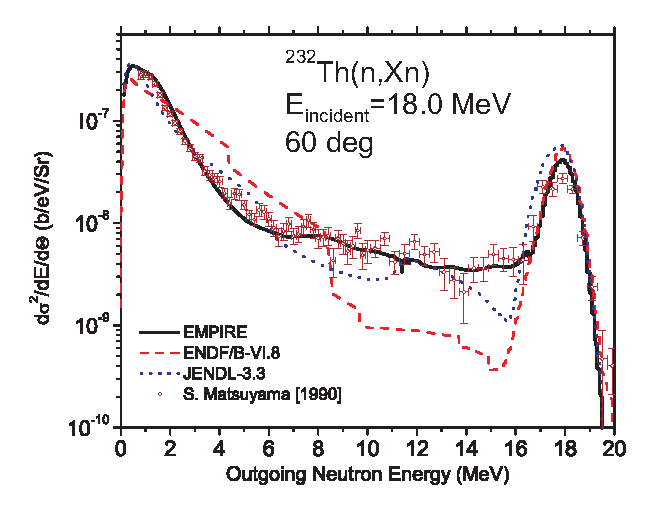
\includegraphics{thorium.eps}}
\caption{EMPIRE calculation for the neutron spectra emission at 60 degree for an incident neutron
 energy of 18.0~MeV on $^{232}$Th, compared to experimental data~\cite{mats} and the ENDF/B-VI.8 and
JENDL-3.3 libraries.}
\label{thoriumMSD}
\end{figure}



%%%%%%%%%%%%%%%%%%%%%%%%%%%%%%%%%%%%%%%%%%%%%%%%%%%%%%%%%%%%%%%%%%%%%%%%%%%%%%%%%%%%%%%%%%%%%%%%%%%%%%%%%%%%%%%%%%
\subsubsection{Exciton model \label{DEGAS}}

\paragraph{DEGAS}
The module DEGAS\index{DEGAS} is the exciton model
code with angular-momentum conservation written by E. B\v et\' ak
as an improved version of the code PEGAS \cite{Degas} by E. B\v et\' ak
and P. Oblo\v zinsk\' y.  Certain features of the DEGAS code
were intentionally disabled for compatibility with other models.
%present in the EMPIRE code.
Thus, $\gamma$-cascade has been limited to primary
$\gamma$s in the composite nucleus and multiple preequilibrium emissions
have been blocked. In particular, DEGAS treatment of the equilibrium
emission was disabled and left to the Hauser-Feshbach\index{Hauser-Feshbach}
model.
% coded in EMPIRE.
Within the above simplifications DEGAS\index{DEGAS} solves the classical
(apart of spin) set of master equations
\begin{eqnarray}
\frac{dP(E,J,n,t)}{dt} & = & P(E,J,n-2,t)\lambda^{+}(E,J,n-2)\nonumber \\
 & + & P(E,J,n+2,t)\lambda^{-}(E,J,n+2)\nonumber \\
 & + & P(E,J,n,t)\left[\lambda^{+}(E,J,n)\right]\nonumber\\
 & + & P(E,J,n,t)\left[\lambda^{-}(E,J,n)+L(E,J,n)\right]\label{mastereq}\nonumber\\
 & + & \sum_{J^{'},n^{'},x}\int P(E^{'},J^{'},n^{'},t)\lambda_{x}\nonumber\\
 &&\text{x} \left(\left[E^{'},J^{'},n^{'}\right]\rightarrow\left[E,J,n\right]\right)d\varepsilon,
\end{eqnarray}
\noindent where $P(E,J,n,t)$ is the occupation probability of the composite
nucleus at the excitation energy $E$, spin $J$ and the exciton number
$n$, $\lambda^{+}$ and $\lambda^{-}$ are the transition rates for
decay to neighboring states, and $L$ is the total integrated emission
rate for particles (protons $\pi$ and neutrons $\nu$) and $\gamma$-rays.
Note, that the last term ensures coupling of different spins. The
nucleon emission rate per energy and time is
\begin{eqnarray}
\lambda_{\pi,\nu}\left(\left[E,J,n\right]\rightarrow\left[U,S,n-1\right]\right)&=&\\
\frac{1}{h}\frac{\omega(n-1,U,S)}{\omega(n,E,J)}\Re_{\pi,\nu}(n)&\text{x}& \sum_{j=\mid S-1/2\mid}^{S+1/2}\sum_{l=\mid J-j\mid}^{J-j}T_{l}(\varepsilon),\nonumber
\end{eqnarray}
\noindent where $\omega(n,E,J)$ is the particle-hole state density, $T_{l}$s
are the transmission coefficients of the emitted nucleon, and $\Re_{x}(n)$
is a fraction of $x$-type nucleons in the $n$-th stage. The particle-hole
state density is
\begin{equation}
\omega(n,E,J)=\frac{g(gE-A_{p,h})^{n}}{p!h!(n-1)!}R_{n}(J),
\end{equation}
\noindent where $g$ is the single-particle level density\index{p-h level densities}y,
$p$ and $h$ are number of particles and holes ($n=p+h$), and $A_{p,h}$
is the Pauli correction term. The spin distribution reads
\begin{equation}
R_{n}(J)=\frac{2J+1}{2}exp\left(-\frac{(J+1/2)^{2}}{2\sigma_{n}^{2}}\right),
\end{equation}
 with $\sigma_{n}$ being the spin cut-off parameter ($\sigma_{n}^{2}=(0.24+0.0038\cdot E)\cdot nA^{2/3}).$
Treatment of the intranuclear cascade rates follows the FKK \cite{FKK}
approach. The energy and spin dependence are assumed to factorize
\begin{equation}
\lambda^{\pm}(E,J,n)=\frac{2\pi}{\hbar}|M|^{2}Y_{n}^{\downarrow}X_{nJ}^{\downarrow},
\end{equation}
\noindent where $|M|^{2}$ is the energy part of the average squared transition
matrix element of the residual interaction, $Y_{n}^{\downarrow}$
is the energy part of the density of accessible final states,  and
the $X_{nJ}^{\downarrow}$ factor takes care of angular momentum coupling.
The latter two read
\begin{equation}
Y_{n}^{\downarrow}=\frac{g}{2(n+1)}\frac{(gE-A_{p+1,h+1})^{n+1}}{(gE-A_{ph})^{n-1}},
\end{equation}
 and
\begin{equation}
X_{nJ}^{\downarrow}=\frac{1}{R_{n}(J)}\sum_{j_{4}Q}R_{1}(Q)\widetilde{F}(Q)R_{n-1}(j_{4})\Delta(Qj_{4}J),
\end{equation}
 with $\Delta(Qj_{4}J)=1$ for $|Q-j_{4}|\leq J\leq Q+j_{4}$ and
0 otherwise. The function $\widetilde{F}(Q)$ is given by
\begin{equation}
\widetilde{F}(Q)=\sum_{j_{3}j_{5}}(2j_{5}+1)R_{1}(j_{5})(2j_{3}+1)F(j_{3})\left(\begin{array}{ccc}
j_{5} & j_{3} & Q\\
\frac{1}{2} & 0 & -\frac{1}{2}\end{array}\right)^{2},
\end{equation}
 and the angular momentum density of the pair of states is
\begin{equation}
F(j_{3})=\sum_{j_{1}j_{2}}(2j_{1}+1)R_{1}(j_{1})(2j_{2}+1)R_{1}(j_{2})\left(\begin{array}{ccc}
j_{1} & j_{2} & j_{3}\\
\frac{1}{2} & -\frac{1}{2} & 0\end{array}\right)^{2}.
\end{equation}
The averaged squared matrix element $|M|^{2}$ is related to the spin-independent
estimate of Kalbach \cite{Kalbach}
\begin{equation}
|M_{nonspin}|^{2}=KA^{-1/3}\varepsilon^{-1},
\end{equation}
\noindent where $\varepsilon=E/n$ is the energy per single exciton. The more
complicated expressions \cite{Kalbach} are used if $\varepsilon$
is outside the 7-15 MeV range. In the current, spin-dependent formulation
the averaged squared matrix element is chosen in such a way that,
after performing additional averaging over spin, the non-spin value
is recovered
\begin{equation}
|M|^{2}\left\langle X_{nJ}^{\downarrow}\right\rangle =|M_{\text{non spin}}|^{2}.
\end{equation}
\begin{figure}[htbp]
\scalebox{0.8}{\includegraphics{ir193.eps}}
\caption{Neutron capture cross section for $^{193}$Ir. }
\label{ir193}
\end{figure}

For the $K$ constant the standard value of 100 MeV$^{3}$ is adopted.
The coding of $\gamma$-emission makes use of the Brink-Axel hypothesis
\cite{Axel,Brink,Brinka} and Giant Dipole Resonance $\gamma$-ray
strength function for the $E1$ transitions. In the angular momentum
coupling formalism the $\gamma$ emission rate $\lambda_{\gamma}$
from an $n$-exciton state is
\begin{eqnarray}
\lambda_{\gamma}\left(\left[E,J,n\right]\rightarrow\left[E-E_{\gamma},S,n\right]\right)&=&\\
\frac{E_{\gamma}^{2}\sigma_{GDR}(E_{\gamma})}{3\pi^{2}\hbar^{3}c^{2}}&\times&\frac{b_{nS}^{nJ}\omega(n,E-E_{\gamma},S)}{\omega(n,E,J)}
\nonumber,
\end{eqnarray}
 if emission of a $\gamma$ occurs with no change in the exciton number,
or
\begin{eqnarray}
\lambda_{\gamma}\left(\left[E,J,n\right]\rightarrow\left[E-E_{\gamma},S,n-2\right]\right)&=&\nonumber\\
\frac{E_{\gamma}^{2}\sigma_{GDR}(E_{\gamma})}{3\pi^{2}\hbar^{3}c^{2}}&\times&\nonumber\\
\frac{b_{n-2,S}^{nJ}\omega(n-2,E-E_{\gamma},S)}{\omega(n,E,J)},&&
\end{eqnarray}
 in the case of annihilation of one particle-hole pair. The photoabsorption
cross section $\sigma_{GDR}(E_{\gamma})$ is written in the Lorentzian
form
\begin{equation}
\sigma_{GDR}(E_{\gamma})=53.2mb\frac{NZ}{A}\frac{E_{\gamma}^{2}\Gamma^{2}}{\left(E_{\gamma}^{2}-E_{GDR}^{2}\right)^{2}+E_{\gamma}^{2}\Gamma^{2}},
\end{equation}
with $\Gamma=5$ MeV and
\begin{equation}
E_{GDR}=29\sqrt{\left(1+2/A^{1/3}\right)/A^{1/3}}\,\,[MeV].
\end{equation}
 The branching ratios are
\begin{equation}
b_{nS}^{nJ}=\frac{y_{m}^{n}x_{mS}^{nJ}}{y_{m}^{m}x_{mS}^{mJ}+y_{m}^{m+2}x_{mS}^{m+2,J}},
\end{equation}
\noindent where
\begin{eqnarray}
y_{n}^{n} & = & gn,\nonumber \\
y_{n}^{n+2} & = & g^{2}\varepsilon,
\end{eqnarray}
and the spin coupling terms read
\begin{eqnarray}
x_{nS}^{nJ} & = & \frac{3(2J+1)}{R_{n}(S)}\nonumber\\
& \times &\sum_{j_{1}j_{2}j_{3}}(2j_{1}+1)R_{1}(j_{1})(2j_{2}+1)R_{1}(j_{2})R_{n-1}(j_{3})\nonumber \\
 & \times & \left(\begin{array}{ccc}
j_{2} & 1 & j_{1}\\
\frac{1}{2} & 0 & -\frac{1}{2}\end{array}\right)^{2}\left\{ \begin{array}{ccc}
j_{2} & j_{3} & S\\
J & 1 & j_{1}\end{array}\right\} ^{2}
\end{eqnarray}
and
\begin{eqnarray}
x_{nS}^{n+2,J}&=&\frac{2J+1}{2S+1}\nonumber\\
&\times&\sum_{j_{1}j_{2}}(2j_{1}+1)R_{1}(j_{1})(2j_{2}+1)R_{1}(j_{2})\nonumber\\
&\times&\left(\begin{array}{ccc}
j_{2} & j_{1} & 1\\
\frac{1}{2} & -\frac{1}{2} & 0\end{array}\right)^{2}\Delta(S1J).
\end{eqnarray}
DEGAS\index{DEGAS} solves the set of master equations (Eq. \ref{mastereq})
and calculates integrals of occupation probabilities
\begin{equation}
\tau(E,J,n)=\int_{0}^{\infty}P(E,J,n,t)dt,
\end{equation}
and preequilibrium emission cross sections
\begin{eqnarray}
\frac{d\sigma_{x}}{d\varepsilon_{x}}&=&\sum_{J_{c},J_{r},n}\int\sigma(E_{c},J_{c})\tau(E_{c},J_{c},n)\lambda_{x}\nonumber\\
&\times&\left(\left[E_{c},J_{c},n\right]\rightarrow\left[E_{r},J_{r},n-1\right]\right)dE_{r}.
\end{eqnarray}
Here, subscripts $c$ and $r$ refer to the composite and residual
nuclei respectively.

An example of an improved calculation of neutron capture reaction on $^{193}$Ir is presented
in Fig.~\ref{ir193}. Two calculations, with and without the DEGAS modelization shows the increase
of the capture cross section above 3~MeV.



\paragraph{PCROSS}
The module PCROSS includes a preequilibrium mechanism for clusters in the incoming and outgoing
channels by including the Iwamoto-Harade model~\cite{Iwamoto} parameterized and improved
in~\cite{Sato,Zhang1,Zhang2}. In this model, the formation probability of a cluster takes into
account excitons below and above the Fermi surface and avoids free parameters. In Fig.~\ref{goldna},
the Iwamoto-Harada model brings an essential improvement into the treatment of the $\alpha$-particle
 emission in the $^{197}$Au(n,$\alpha$) reaction.
\begin{figure}[htbp]
\scalebox{0.61}{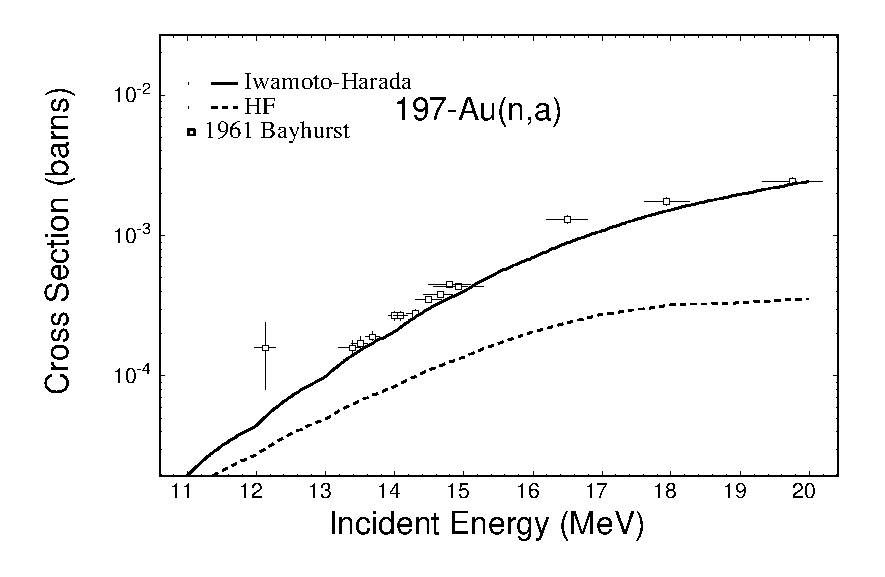
\includegraphics{hermanm1_f4.eps}}
\caption{Improvement achieved with the Iwamoto-Harada model for $^{179}$Au(n,$\alpha$) reaction.}
\label{goldna}
\end{figure}




%%%%%%%%%%%%%%%%%%%%%%%%%%%%%%%%%%%%%%%%%%%%%%%%%%%%%%%%%%%%%%%%%%%%%%%%%%%%%%%%%%%%%%%%%%%%%%%%%%%%%%%%%%%%%%%%%%
\subsubsection{Monte Carlo Preequilibrium\label{DDHMS}}
The Hybrid Monte-Carlo Simulation (HMS) approach to the preequilibrium
emission of nucleons  has
been formulated by M. Blann \cite{Blann-HMS} as a hybrid model
\cite{hybrid,hybrid1,hybrid2,hybrid3}
inspired version of the intranuclear cascade approach. Contrary to
other classical preequilibrium models, this approach avoids multi-exciton
level densities\index{p-h level densities}, which were shown by Bisplinghoff
\cite{Bisplinghoff} to be used inconsistently in the exciton and
in the hybrid formulations. The HMS\index{HMS} model has a number
of attractive features. First of all, there are no physical limits
on a number of preequilibrium emissions (apart from energy conservation).
With the addition of linear momentum conservation by M. Chadwick and
P. Oblo\v zinsk\' y (DDHMS), the model provides a nearly complete
set of observables. These include cross sections for the production
of residuals, light-particle double-differential spectra and spectra
of recoils. Spin and excitation-energy dependent populations of residual
nuclei can also be obtained, an essential feature for coupling the
preequilibrium mechanism to the subsequent Compound Nucleus decay.
The binding energies in the HMS\index{HMS} model are thermodynamically
correct. The DDHMS model proved to perform very well
%up to at least 250 MeV, extending energy range of the EMPIRE applicability
up to at least 250 MeV.
%to the desired limit.
The calculation flow in the DDHMS model can be summarized in terms
of the following steps:
\begin{enumerate}
\item draw collision partner for the incoming nucleon (2p-1h state created)
\item draw energy ($\varepsilon$) of the scattered nucleon (if bound go
to step 5)
\item draw scattering angles for both particles
\item decide whether the scattered nucleon will be emitted, re-scattered
or trapped
\begin{enumerate}
\item if emitted appropriate cross section is augmented
\item if re-scatters additional particle-hole is created and we return to
step 2
\item if trapped, go to step 5
\end{enumerate}
\item draw excitation energy of a particle in the remaining 1p-1h configuration
(between 0$\div(U-\varepsilon)$), if unbound go to step 3, if bound
choose another existing 1p-1h pair and repeat step 5.
\end{enumerate}

\begin{figure}[htbp]
\scalebox{0.75}{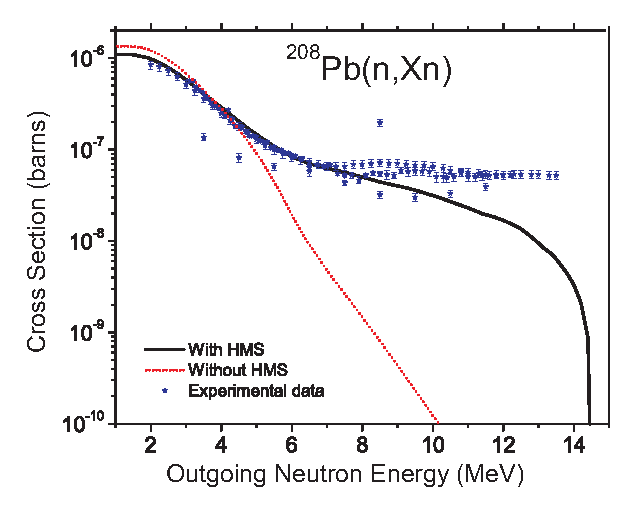
\includegraphics{pb208.eps}}
\caption{Neutron emission for $^{208}$Pb(n,xn) reaction with and without HMS.}
\label{pb208HMS}
\end{figure}




All excitons (including holes) are treated on equal footing and each
of them is given a chance to interact or being emitted with \emph{a
priori} equal probability. The cascade ends when all excitons are
bound. Below, we summarize various probability distributions which
are used in concert with a random number generator.
For choosing a collision partner it is assumed that the unlike interaction
is 3 times more probable than the like one ($\sigma_{np}=3\sigma_{nn}$).
Thus, for the incident neutron we have $P_{nn}$ and $P_{np}$ for
the probability of exciting neutron and proton respectively
\begin{equation}
P_{nn}=\frac{(A-Z)}{(A-Z)+3Z},\label{Pnn}\end{equation}

\begin{equation}
P_{np}=1-P_{nn}\label{Pnp}\end{equation}
 and similarly for the incident proton
\begin{equation}
P_{pp}=\frac{Z}{Z+3(A-Z)},\label{Ppp}\end{equation}
\begin{equation}
P_{pn}=1-P_{pp}.\label{Ppn}\end{equation}
The energy distribution of the scattered particles $P(\varepsilon)$
is given by the ratio of the $(n-1)-$ and $n$-exciton level densities\index{p-h level densities}
$\rho_{n}$
\begin{equation}
P(\varepsilon)d\varepsilon=\frac{\rho_{n-1}(E-\varepsilon)g}{\rho_{n}(E)}d\varepsilon,\label{Penergy}\end{equation}
with $n=2\, or\,3$ and\begin{equation}
\rho_{2}(E)=\frac{g(gV)}{2}\,\,\, if\,\,\, E>V,\label{ro2u}\end{equation}
\begin{equation}
\rho_{2}(E)=\frac{g(gE)}{2}\,\,\, if\,\,\, E\leq V,\label{ro2d}\end{equation}
\begin{equation}
\rho_{3}(E)=\frac{g^{3}\left[V(2E-V)\right]}{4}\,\,\, if\,\,\, E\geq V.\label{ro3}\end{equation}
 Here, $V$ is a potential well depth. The emission probability is
calculated as
\begin{equation}
P_{\nu}(\varepsilon-Q)=\frac{\lambda_{c}(\varepsilon-Q)}{\lambda_{c}(\varepsilon-Q)+\lambda_{+}(\varepsilon)},\label{Pnu}\end{equation}
with the emission rate being
\begin{equation}
\lambda_{c}(\varepsilon-Q)\sim\frac{\sigma_{\nu}(\varepsilon-Q)(\varepsilon-Q)(2S+1)\mu_{\nu}}{g}.\label{lambdac}\end{equation}
$\sigma_{\nu}$ is an inverse reaction cross section, $Q$ is a binding
energy, $g$ is a single particle density, $S$ denotes nucleon spin,
and $\mu_{\nu}$ stands for the reduced nucleon mass. Following the
hybrid\index{HYBRID} model, $\lambda_{+}(\varepsilon)$ is calculated
from the mean free path of a nucleon in nuclear matter.
The version which is actually implemented in EMPIRE has been coded
by M. Chadwick and extended to double-differential cross sections
in collaboration with P. Oblo\v zinsk\' y \cite{DDHMScode}.

Figure~\ref{pb208HMS} presents two calculations, with and without (compound nucleus only) the HMS model for the
neutron emission on $^{208}$Pb at an incident neutron energy of 14.6~MeV. A good agreement is obtained in the
case of the HMS calculation.



%%%%%%%%%%%%%%%%%%%%%%%%%%%%%%%%%%%%%%%%%%%%%%%%%%%%%%%%%%%%%%%%%%%%%%%%%%%%%%%%%%%%%%%%%%%%%%%%%%%%%%%%%%%%%%%%%%
\subsection{Compound Reactions}


%The statistical model used in the EMPIRE is an advanced implementation
The statistical model used in the EMPIRE is an advanced implementation
of the Hauser-Feshbach\index{Hauser-Feshbach} theory. The exact angular
momentum and parity coupling is observed. The emission of neutrons,
protons, $\alpha$-particles, and a light ion is taken into account
along with the competing fission channel. The full $\gamma$-cascade
in the residual nuclei is considered. Particular attention is dedicated
to the determination of the level densities\index{level densities},
which can be calculated in the non-adiabatic approach allowing for
the rotational and vibrational enhancements. These collective effects
are gradually removed above a certain energy. Level densities acquire
dynamic features through the dependence of the rotational enhancement
on the shape of a nucleus.
In the frame of the statistical model of nuclear reactions the contribution
of the Compound Nucleus (CN) state $a$ with spin $J$, parity $\pi$,
and excitation energy $E$ to a channel $b$ is given by the ratio
of the channel width $\Gamma_{b}$ to the total width $\Gamma_{tot}=\sum_{c}\Gamma_{c}$
multiplied by the population of this state $\sigma_{a}(E,J,\pi)$.
This also holds for secondary CNs that are formed due to subsequent
emissions of particles. The only difference is that while the first
CN is initially excited to the unique (incident channel compatible)
energy, the secondary CNs are created with excitation energies which
spread over the available energy interval. Each such state contributes
\noindent
\begin{equation}
\sigma_{b}(E,J,\pi)=\sigma_{a}(E,J,\pi)\frac{\Gamma_{b}(E,J,\pi)}{\sum_{c}\Gamma_{c}(E,J,\pi)}
\label{Hauser}
\end{equation}
to the cross section. These have to be summed over spin $J$ and parity
$\pi$, and integrated over excitation energy $E$ (in case of daughter
CN) to obtain observable cross sections. The particle decay width
is given by
\begin{eqnarray}
\Gamma_{c}(E,J,\pi)&=&\frac{1}{2\pi\rho_{CN}(E,J,\pi)}\nonumber\\
&\times&\sum_{J'=0}^{\infty}\sum_{\pi'}\sum_{j=J'-J}^{J+J'}\int_{0}^{E-B_{c}}\rho_{c}(E',J',\pi')\nonumber\\
&\times&T_{c}^{l,j}(E-B_{c}-E')dE',\label{pwidth}
\end{eqnarray}
\noindent where $B_{c}$ is the binding energy of particle $c$ in
the compound nucleus, $\rho$ is the level density\index{level density},
and $T_{c}^{l,j}(\epsilon)$ stands for the transmission coefficient
for particle $c$ having channel energy $\epsilon=E-B_{c}-E'$ and
orbital angular momentum $l$, which together with the particle spin
$s$ couples to the channel angular momentum $j$. For the discrete
levels (characterized by the energy $E_{i}$, spin $J_{i}$, and parity
$\pi_{i}$) the level density $\rho(E,J',\pi')$ reduces to $\delta(E-E_{i})\delta_{(J',J_{i})}\delta_{(\pi',\pi_{i})}$.
The parity selection rules are implicit in
Eq. \ref{pwidth}.

\subsubsection{Level densities}
EMPIRE accounts for various models describing level densities\index{level densities}
and includes several respective parameterizations. In each case equal
parity distribution $\rho(E,J,\pi)=\frac{1}{2}\rho(E,J)$ is assumed.
Choice of the proper representation depends on a case being considered.
For the nucleon induced reactions, with CN excited up to about 20
MeV, the Gilbert-Cameron approach is recommended. It assures the most
accurate description of level densities in the energy range up to
the neutron binding energy. The collective effects are included in
the level density parameter $a$, providing reasonable estimate of
the level densities as long as damping of the collective effects is
irrelevant. The relatively low angular momentum introduced by the
incident projectile justifies neglect of dynamical effects.

\paragraph{Gilbert-Cameron level densities}
The Gilbert-Cameron approach \cite{gc} splits excitation energy in
two regions. Different functional forms of level densities\index{level densities}
are applied in each of them. At low excitation energies (below the
matching point $U_{x}$) the constant temperature formula is used
\begin{equation}
\rho_{T}(E)=\frac{1}{T}exp\left[(E-\Delta-E_{0})/T\right],
\label{lgcld}
\end{equation}
\noindent where $T$ is the nuclear temperature, $E$ is the excitation energy
($E=U+\Delta$ with $\Delta$ being the pairing correction), and $E_{0}$
is an adjustable energy shift. Above $U_{x}$ the Fermi gas formula
is applied
\begin{equation}
\rho_{F}(U)=\frac{exp(2\sqrt{aU})}{12\sqrt{2}\sigma^3(U)a^{1/4}U^{5/4}}.
\label{ferld}
\end{equation}
The level density parameter $a$ is assumed to be energy independent.
The spin cut-off factor $\sigma(U)$ is given by
\begin{equation}
\sigma^{2}(U)=0.146A^{2/3}\sqrt{aU}.
\label{sigld}
\end{equation}
Three model parameters, $T,\, U_{x},$ and $E_{0}$, are determined
by the requirement that the level density and its derivative are continuous
at the matching point $U_{x}$, and by fitting cumulative number of
discrete levels with the integral of Eq. \ref{lgcld}. The first of
the conditions implies
\begin{equation}
\frac{1}{T}=\sqrt{a/U_{x}}-\frac{3}{2U_{x}}.
\label{condUT}
\end{equation}
The systematics of the level density parameter $a$ used by EMPIRE,
account for the shell effects, which fade-out
with increasing energy implying energy dependence of the $a$ parameter.
The general form of this dependence was proposed by Ignatyuk~\cite{ignaa}
\begin{equation}
a(U)=\widetilde{a}[1+f(U)\frac{\delta W}{U}],
\label{apiccoloGC}
\end{equation}
\noindent where $\delta W$ is the shell correction, $\widetilde{a}$ is the
asymptotic value of the $a$-parameter and
\begin{equation}
f(U)=1-exp(-\gamma U).
\label{shellGC}
\end{equation}
The three relevant systematics available in EMPIRE are:
(i) Ignatyuk \emph{et al.} \cite{ignaa}: $\widetilde{a}=0.154A+6.3\cdot10^{-5}A^{2}$
and $\gamma=-0.054$
(ii) Arthur \cite{arthura}: $\widetilde{a}=0.1375A-8.36\cdot10^{-5}A^{2}$
and $\gamma=-0.054$
(iii) Iljinov \emph{et al.} \cite{Mebel}: $\widetilde{a}=0.114A+9.80\cdot10^{-2}A^{2/3}$
and $\gamma=-0.051$
We stress that Gilbert-Cameron approach does not account explicitly
for the collective enhancements of the level densities\index{level densities}.
These are included implicitly in the $\widetilde{a}$ when fitting
neutron resonance spacings. Such an approach leads to the over-estimation
of the level densities above, say, 20 MeV.

\paragraph{EMPIRE-specific level densities}
The dynamic approach to the level densities\index{level densities}
is specific to the EMPIRE code. It takes into account collective enhancements
of the level densities due to nuclear vibration and rotation. The
formalism uses the super-fluid model below critical excitation energy
and the Fermi gas model above. Differently from other
similar formulations, the latter one accounts explicitly for the rotation
induced deformation of the nucleus, which becomes spin dependent.
The deformation enters level densities
formulas through moments of inertia and through the level density
parameter \emph{a} that increases with increase in the surface of
the nucleus.
Assuming that the prolate nuclei rotate along the axis perpendicular
to the symmetry axis the explicit level density formulas reads
\begin{eqnarray}
\rho(E,J,\pi) & = & \frac{1}{16\sqrt{6\pi}}\left(\frac{\hbar^{2}}{\Im_{\Vert}}\right)^{\frac{1}{2}}a^{1/4}\sum_{K=-J}^{J}\left(U-\frac{\hbar^{2}K^{2}}{2\Im_{eff}}\right)^{-\frac{5}{4}}\nonumber \\
 &  & \exp\left\{ 2\left[a\left(U-\frac{\hbar^{2}K^{2}}{2\Im_{eff}}\right)\right]^{\frac{1}{2}}\right\} .\label{ro1}
\end{eqnarray}
In the case of the oblate nuclei which are assumed to rotate parallel
to the symmetry axis we have
\begin{eqnarray}
\rho(E,J,\pi) & = & \frac{1}{16\sqrt{6\pi}}\left(\frac{\hbar^{2}}{\Im_{\Vert}}\right)^{\frac{1}{2}}a^{1/4}\nonumber \\
 &  & \sum_{K=-J}^{J}\left(U-\frac{\hbar^{2}\left[J\left(J+1\right)-K^{2}\right]}{2|\Im_{eff}|}\right)^{-\frac{5}{4}}\label{ro2}\\
 &  & \exp\left\{ 2\left[a\left(U-\frac{\hbar^{2}\left[J\left(J+1\right)-K^{2}\right]}{2|\Im_{eff}|}\right)\right]^{\frac{1}{2}}\right\} .\nonumber
 \end{eqnarray}
$a$ is a level density\index{level density} parameter, $J$ is a
nucleus spin and $K$ its projection, $E$ is the excitation energy
and $U$ is the excitation energy less pairing ($\Delta$). The effective
moment of inertia $\Im_{eff}$ is defined in terms of the perpendicular
$\Im_{\Vert}$and parallel $\Im_{\bot}$moments through the difference
of their inverses
\begin{equation}
\frac{1}{\Im_{eff}}=\frac{1}{\Im_{\Vert}}-\frac{1}{\Im_{\bot}}.\label{mom-iner}
\end{equation}
The saddle-point moments of inertia are calculated using Sierk's routine
MOMFIT \cite{sierk}, which provides a fit to the advanced liquid-drop
model calculations.
It should be stressed that Eqs. \ref{ro1} and \ref{ro2} include
summation over projection of the angular momentum $K$ and thus automatically
account for the rotational enhancement. The yrast line is obtained,
setting level densities to 0 whenever the
rotational energy becomes larger than $U$. In addition to the rotational
enhancement the model accounts also for the vibrational enhancement.
To this end Eqs. \ref{ro1} and
\ref{ro2} are multiplied by $K_{vib}$
\begin{equation}
K_{vib}=exp\left\{ 1.7\left(\frac{3m_{0}A}{4\pi h^{2}S_{drop}}\right)^{2/3}T^{4/3}\right\} \label{Kvib}
\end{equation}
with $S_{drop}=17/4\pi r_{^{2}0}$ and $r_{0}=1.26$.
Damping of the rotational enhancement is achieved by multiplying Eqs.
\ref{ro1} and \ref{ro2} by
\begin{equation}
1-Q_{rot}\left(1-\frac{1}{\hbar^{2}/\Im_{\bot}t}\right)\label{damp}
\end{equation}

\noindent where $Q_{rot}=2/\left[\exp(E_{cor}/t)+1\right]$ is a damping function
which tends to 0 for low temperatures $t$, and approaches 1 for $t\rightarrow\infty$.
The Coriolis energy is given by
\begin{equation}
E_{cor}\simeq\hbar\omega_{0}\mid\delta_{osc}\mid=41A^{-1/3}\mid\delta_{osc}\mid.\label{Coriolis}
\end{equation}


\noindent Following Junghans \emph{et al.} \cite{Ignadamp} $Q_{rot}$
is assumed to be deformation independent
\begin{equation}
Q_{rot}=\frac{1}{1+exp\left(-\frac{E_{cr}}{d_{cr}}\right)}-\frac{1}{1+exp\left(-\frac{E-E_{cr}}{d_{cr}}\right)}\label{Qrot}
\end{equation}
 \noindent with $E_{cr}=40$ MeV and $d_{cr}=10$ MeV. The two terms
in Eq. \ref{Qrot} ensure that $Q_{rot}=0$ at $E=0$ and tends to
1 for $E\rightarrow\infty$. We note that $\hbar^{2}/\Im_{\bot}t$
is approximately equal to the rotational enhancement and therefore
multiplication of the level densities\index{level densities} by Eq.
\ref{damp} actually removes rotational enhancement when $Q_{rot}=1$.
As nuclear temperature $T$ increases the vibrational enhancement
is damped by multiplying Eqs. \ref{ro1} and \ref{ro2} by the factor
\begin{equation}
Q_{vib}=exp^{-1}\left(1-\frac{T-T_{1/2}}{DT}\right)\,.\label{Qvib}
\end{equation}
 $T_{1/2}=1$ MeV and $DT=0.1$ MeV are taken as default.

The low-energy part of level densities
is calculated in terms of the super-fluid (BCS\index{BCS}) model
\cite{igna}. With the pairing gap $\Delta=12/\sqrt{A}$ the critical
temperature $T_{crt}$ is
\begin{equation}
T_{crt}=0.567\Delta.\label{Tcrt}
\end{equation}
The critical value of the level density parameter \emph{a} is then
determined by the iteration procedure
\begin{equation}
a_{crt}^{(0)}=\widetilde{a}\left(1+\gamma\delta_{W}\right)\label{ait0}
\end{equation}
\begin{equation}
U^{(n)}=a_{crt}^{(n)}T_{crt}^{2}\label{Uit}
\end{equation}
\begin{equation}
a_{crt}^{(n+1)}=\widetilde{a}\left[1+\frac{\delta_{W}}{U^{(n)}}\left(1-\exp\left(-\gamma U^{(n)}\right)\right)\right]\,.\label{ait}
\end{equation}
$\widetilde{a}$ is the asymptotic value of the level density parameter.
Eqs. \ref{Uit} and \ref{ait} are iterated until the condition
\begin{equation}
\frac{\left|a^{(n+1)}-a^{(n)}\right|}{a^{(n+1)}}<0.001\label{itercond}
\end{equation}
is fulfilled. The condensation energy $E_{cond}$, critical energy
$U_{crt}$, a critical value of the determinant $Det_{crt}$, and
critical entropy $S_{crt}$ are defined by the following expressions
\begin{equation}
E_{cond}=1.5a_{crt}\Delta^{2}/\pi^{2},\label{Econd}
\end{equation}
\begin{equation}
U_{crt}=a_{crt}T_{crt}^{2}+E_{cond}\,,\label{Ucrt}
\end{equation}
\begin{equation}
Det_{crt}=\left(\frac{12}{\sqrt{\pi}}\right)^{2}a_{crt}^{3}T_{crt}^{5}\,,\label{Detcrt}
\end{equation}
\begin{equation}
S_{crt}=2a_{crt}T_{crt}\,.\label{Scrt}
\end{equation}
At excitation energies below $U_{crt}$ ({\it i.e.}, in the energy range
\noindent where the BCS\index{BCS} model applies) we define the parameter $\varphi$
\begin{equation}
\varphi=\sqrt{1-U/U_{crt}}\,,\label{fiign}
\end{equation}
which allows to express all thermodynamical quantities in terms of
their critical values
\begin{equation}
T=2T_{crt}\varphi\ln^{-1}\left(\frac{\varphi+1}{1-\varphi}\right)\,,\label{Tign}
\end{equation}
\begin{equation}
S=S_{crt}T_{crt}(1-\varphi^{2})/T\,,\label{Sign}
\end{equation}
\begin{equation}
Det=Det_{crt}(1-\varphi^{2})(1+\varphi^{2})^{2}\,.\label{Detign}
\end{equation}
The parallel and orthogonal moments of inertia below the critical
temperature $T_{crt}$ are
\begin{equation}
\Im_{\parallel}^{BCS}=\Im_{\parallel}T_{crt}(1-\varphi^{2})/T\label{momparign}
\end{equation}
and
\begin{equation}
\Im_{\perp}^{BCS}=\frac{1}{3}\Im_{\perp}+\frac{2}{3}\Im_{\perp}T_{crt}(1-\varphi^{2})/T\label{momortign}
\end{equation}
respectively (see the following section for the definitions of $\Im_{\parallel}$
and $\Im_{\perp}$). Using these results squares of the effective
spin cut-off parameters are defined as
\begin{equation}
\begin{array}{ll}
\sigma_{eff}^{2}=\Im_{\parallel}^{BCS}T & \,\,\, for\,\,\alpha_{2}<0.005\,,\\
\sigma_{eff}^{2}=\left(\Im_{\parallel}^{BCS}\right)^{1/3}\left(\Im_{\perp}^{BCS}\right)^{2/3}T & \,\,\, for\,\,\alpha_{2}>0.005\,,\end{array}\label{sigeffign}
\end{equation}
with $\alpha_{2}$ being ground state deformation. The BCS\index{BCS}
level densities\index{level densities} are calculated according to
the expression
\begin{equation}
\rho_{BCS}(U,J)=\frac{2J+1}{2\sqrt{2\pi}\sigma_{eff}^{3}\sqrt{Det}}\exp\left(\frac{S-J(J+1)}{2\sigma_{eff}^{2}}\right)\label{roBCS}
\end{equation}
 Finally, Eq. \ref{roBCS} is corrected for rotational and vibrational
collective effects in the non-adiabatic mode ({\it i.e.}, including their
damping with increasing temperature), that results in
\begin{equation}
\rho(U,J)=\rho_{BCS}(U,J)Q_{rot}^{BCS}K_{rot}Q_{vib}K_{vib}\,.\label{roBCScol}
\end{equation}
The vibrational enhancement $K_{vib}$ and its damping $Q_{vib}$
are given by Eqs. \ref{Kvib} and \ref{Qvib} respectively. The rotational
enhancement is
\begin{equation}
K_{rot}=\Im_{\perp}T\label{KrotBCS}
\end{equation}
and is damped with the function
\begin{equation}
Q_{rot}^{BCS}=1-Q_{rot}\left(1-\frac{1}{\Im_{\perp}T}\right)\,,\label{QrotBCS}
\end{equation}
\noindent where $Q_{rot}$ has been defined by Eq. \ref{Qrot}.
The level density
parameter $a$ is assumed to be energy (temperature)
dependent and calculated following Ignatyuk \emph{et al.} \cite{ignaa}
as
\begin{equation}
a(U)=\widetilde{a}[1+f(U)\frac{\delta_{W}}{U}],\label{apiccolo}
\end{equation}
\noindent where $\delta_{W}$ is the shell correction and $\widetilde{a}$ is
the asymptotic value of the $a$-parameter given by,
\begin{equation}
\widetilde{a}=\eta A+\zeta A^{2/3}F_{surf}(R_{max}/R_{min}),\label{aassym}
\end{equation}
and
\begin{equation}
f(U)=1-exp(-\gamma U).\label{shell}
\end{equation}
Compared to the original formulation of Ignatyuk \emph{et al.} \cite{ignaa},
there is an additional factor $F_{surf}(R_{max}/R_{min})$ in Eq.
\ref{apiccolo}. It accounts for the dependence of the level density
parameter on nuclear deformation. This factor is a function of the
ratio of nuclear axes $R_{max}$ and $R_{min}$ and was provided by
Igor Gontchar \cite{gontchar} in a tabular form .
The level density \emph{a}-parameters at neutron binding energy $a_{B_{n}}$
were extracted using Eqs. \ref{ro1} through \ref{Qvib} from average
neutron resonance spacings $D_{obs}$ compiled by Iljinov {\it et al.}~\cite{Mebel}.
These \emph{a} values were fitted with Eqs. \ref{apiccolo} through
\ref{shell} to obtain \emph{$\eta$, $\zeta$,} and \emph{$\gamma$}
parameters. Depending on the choice of shell-corrections the two sets
of parameters were derived. For the Nix-Moller shell corrections \cite{masses}
the parameters are:
\begin{equation}
\begin{array}{ccccccc}
\eta= & 0.094431 &  & \eta= & 0.117113\\
\xi= & -0.08014 & for\, Z<85 & \xi= & -0.09939 & for\, Z\geq85\\
\gamma= & 0.075594 &  & \gamma= & 0.094447\end{array}\end{equation}
When Myers-Swiatecki shell-corrections are being used the parameters
become:\begin{equation}
\begin{array}{ccc}
\eta= & 0.052268\\
\xi= & 0.13395 & for\, Z<85\\
\gamma= & 0.093955\end{array}\begin{array}{ccc}
\eta= & 0.067645\\
\xi= & 0.173358 & for\, Z\geq85\\
\gamma= & 0.121465\end{array}\end{equation}
Actually, EMPIRE looks in the \emph{data/ldp.dat} file for the experimental
values of the $a$-parameter. Experimental results are given priority
over the systematics prediction. The average ratio of the experimental
values to the results of Eq. \ref{aassym} is used to normalize systematics
predictions for the nuclei for which there are no experimental results.
This way a sort of the \char`\"{}local systematics\char`\"{} is constructed
for the nuclei involved in the calculation run. In both cases, level
densities\index{level densities} below $U_{crt}$ are calculated
in the frame of the super-fluid model \cite{igna} with the pairing
gap $\Delta=12/\sqrt{A}$.

\paragraph{Hartree-Fock-BCS level densities}
EMPIRE can read precalculated level densities\index{level densities}
from the RIPL\index{RIPL}-2 library, which contains tables of level
densities~\cite{HFBCS} for more than 8000 nuclei calculated in the
frame of the Hartree-Fock-BCS approach. These microscopic results
include a consistent treatment of shell corrections, pairing correlations,
deformation effects and rotational enhancement. The results were re-normalized
to the experimental \emph{s}-wave neutron resonance spacings and adjusted
to the cumulative number of discrete levels, so that the degree of
accuracy is comparable to the phenomenological formulae.
Using the partition function method, the state density can be obtained
as
\begin{equation}
\omega(U)=\frac{e^{S(U)}}{(2\pi)^{3/2}\sqrt{Det(U)}}.
\label{statdens}
\end{equation}
 Entropy \emph{S} and excitation energy \emph{U} are derived from
the summation over single particle levels and \emph{Det} stands for
the determinant. Pairing correlations are treated within the standard
BCS theory in the constant-\emph{G} approximation with blocking. Consequently
single-particle energies are replaced by their quasi-particle equivalents
with BCS\index{BCS} equations determining gap parameter $\Delta$
and the chemical potential $\lambda$. Spherical and deformed nuclei
are treated in a distinct mode. The level density\index{level density}
for spherical nuclei is simply related to the state density (Eq. \ref{statdens})
\begin{equation}
\rho_{sph}(U,J)=\frac{2J+1}{2\sqrt{2\pi^{3}}}e^{-J(J+1)/(2\sigma^{2})}\omega(U),
\label{rhosph}
\end{equation}
while for deformed nuclei the formula is similar to the one used in
the EMPIRE-specific level densities (Eqs. \ref{ro1} and \ref{ro2})
\begin{eqnarray}
\rho_{def}(U,J)&=&\frac{1}{2}\sum_{K=-J}^{J}\frac{1}{\sqrt{2\pi\sigma^{2}}}\\
&\times&e^{-[J(J+1)/(2\sigma_{\bot}^{2})+K^{2}(1/\sigma^{2}-1/\sigma_{\perp}^{2})/2]}\omega(U),\nonumber
\label{rhodef}
\end{eqnarray}
in which $\sigma$ is the spin cut-off parameter and $\sigma_{\perp}$the
perpendicular spin cut-off parameter, both affected by the pairing
correlations, and $\sigma_{\perp}$being related to the perpendicular
moment of inertia. It should be stressed that similarly to Eq. \ref{ro1}
and \ref{ro2}, Eq. \ref{rhodef} comprises rotational enhancement.
As in the case of EMPIRE-specific level densities\index{level density},
this enhancement has to disappear with increasing excitation energy.
To this end, a phenomenological damping function $f_{dam}$ is introduced
\begin{equation}
f_{dam}(U)=\frac{1}{1+e^{(U-E_{def})/d_{U}}}\left[1-\frac{1}{1+e^{(\beta_{2}-\beta^{*})/d\beta}}\right]'
\label{dampgor}
\end{equation}
 which contains energy and deformation dependent factors. The deformation
energy is the difference between the energy in the spherical configuration
and at the equilibrium deformation. The parameter $d_{U}$ describes
how fast the sphericity is recovered at energies above $E_{def}=E_{sph}-E_{eq}$.
$\beta^{*}$ defines an actual deformation when moving between spherical
and deformed shape. The above parameters were taken as $d_{U}=2..5$
MeV, $\beta^{*}=0.15$ and $d_{\beta}=0.01$. With this damping function
the level density\index{level density} formula reads
\begin{equation}
\rho(U,J)=\left[1-f_{dam}(U)\right]\rho_{sph}(U,J)+f_{dam}(U)\rho_{def}(U,J).
\label{rogor}
\end{equation}
HF-BCS\index{HF-BCS} calculations depend on the single-particle schemes
used to determine the thermodynamic quantities, in particular on the
single-particle state density around the Fermi energy. The calculations
under discussion are based on schemes obtained using the Hartree-Fock
method with MSk7 Skyrme type force. These single-particle levels perform
very well in predicting nuclear masses and other ground state properties,
which increases the confidence in the level densities\index{level densities}
calculated by this approach.
\begin{figure}[htbp]
\scalebox{0.8}{\includegraphics{levden.eps}}
\caption{Neutron capture cross section for $^{160}$Gd obtained with three different
level density representations.}
\label{levdens}
\end{figure}

 As mentioned earlier, final results were
adjusted to resonance spacings at the neutron binding energy and to
the cumulative number of discrete levels by applying shift to the
excitation energy and a multiplicative factor to the entropy. Therefore,
no further phenomenological adjustment needs to be performed by EMPIRE.
Level density tables contain numerical values for 30 spins and extend
up to 150 MeV, which sets limits on their possible utilization, although
spin restriction should not be an issue for nucleon induced reactions.
Before concluding this section we would like to note certain affinity
between the HF-BCS\index{HF-BCS} and the default, EMPIRE-specific,
level densities\index{level densities}. Both approaches use the BCS\index{BCS}
model at low energies, incorporate rotational enhancement directly
into the level density formula, and apply phenomenological (although
functionally different) damping of rotational effects. Both take into
account deformation effects (in EMPIRE-specific densities these are
not only temperature but also spin dependent), and are adjusted to
the available experimental information. The EMPIRE-specific densities
also include a vibrational enhancement factor. However, the most essential
difference between the two approaches is the use of a phenomenological
\emph{a}-parameter and closed formula in the EMPIRE-specific approach,
while HF-BCS\index{HF-BCS} level densities\index{level densities}
are derived directly from the microscopic single-particle schemes.
The latter approach is expected to be more reliable away from valley
of stability.

A comparison of  calculation of the neutron capture cross section on $^{160}$Gd
with different level densities is presented in Fig.~\ref{levdens}. These
calculations were obtained with default parameters for the models.


\subsubsection{Nuclear deformation and moments of inertia\label{sec: defor}}
The shape of each nucleus affects such parameters as the Giant Dipole
Resonance, level density parameters \emph{a} and rotational enhancement
of the level densities\index{level densities}. This shape is estimated
by the code by summing up ground state deformation and dynamic deformation
induced by the rotation of the nucleus . The ground state deformation
%is read from the file \textit{data/nix-moller.dat} \cite{masses},
is taken from Nix \& Moller~\cite{masses},
and the dynamic deformation is taken to be proportional to the square
of the angular momentum $I$. Ground state deformation $\alpha_{g.s.}$
is damped with the increasing nuclear temperature, since nuclei are
known to become spherical at high excitation energies. The dynamic
deformation $\alpha_{2dyn}$ is calculated following Vigdor and Karwowski
\cite{VK}
\begin{equation}
\alpha_{2dyn}\approx b(-1.25y/(1-x)),
\label{defor}
\end{equation}
\noindent where $b$ is treated as an adjustable parameter. The angular momentum
parameter $y$ is given by
\begin{equation}
y=1.9249I(I+1)\frac{I(I+1)}{\eta A^{7/3}}
\end{equation}
and the fissility parameter is given by
\begin{equation}
x=0.01965\frac{Z^{2}}{\eta A},
\end{equation}
\noindent where $\eta$ is the neutron-proton difference term
 \begin{equation}
\eta=1-1.7826(N-Z)^{2}A^{-2}.
\end{equation}
 Accordingly, the deformation is parametrized as
\begin{equation}
\alpha_{2}(T,I)=\alpha_{g.s.}h(T)+\alpha_{2dyn}
\label{totdefor}
\end{equation}
\noindent where $h(T)=1/\{1+\exp[(T-2)/0.5]\}$ damps the ground state
deformation with increasing excitation and reduces the value by 50~\%
at temperature $T=2$ MeV. This value seems a reasonable estimate
corresponding to about 50 MeV of excitation energy. Obviously, such
a procedure is an approximation, but a more rigorous approach (e.g.
using Cranking Model to determine potential surface minima at different
spins and temperatures) would require prohibitive calculation times,
due to to the large number of intermediate nuclei involved. However,
we believe that the approximation used is sufficient to provide the
leading term of the effect. We note that when using this prescription,
a nucleus that is deformed in the ground state will tend (at low spins)
to become spherical with increasing energy. This is because of the
temperature damping of the ground state and negligible contribution
of the dynamic deformation at low spins. On the other hand, for $b>0$,
a prolate nucleus will tend to become spherical and eventually oblate
with increasing angular momentum. Qualitatively, such behavior agrees
with the results of the more rigorous calculations \cite{and76}.
Moments of inertia for the yrast states (not the saddle-point) are
calculated for deformation $\alpha_{2}(T,I)$ using expressions proposed
by Vigdor and Karwowski \cite{VK}
\begin{eqnarray}
\Im_{\parallel}=\Im_{0}(1-\alpha_{2}+0.429\alpha_{2}^{2}+0.268\alpha_{2}^{3}-0.212\alpha_{2}^{4}\nonumber \\
-1.143\alpha_{2}\alpha_{4}+0.494\alpha_{2}^{2}\alpha_{4}+0.266\alpha_{4}^{2})\label{MOMpar}\end{eqnarray}
\begin{eqnarray}
\Im_{\perp}=\Im_{0}(1+0.5\alpha_{2}+1.286\alpha_{2}^{2}+0.581\alpha_{2}^{3}-0.451\alpha_{2}^{4}\nonumber \\
+0.571\alpha_{2}\alpha_{4}+1.897\alpha_{2}^{2}\alpha_{4}+0.700\alpha_{4}^{2})\label{MOMort}\end{eqnarray}
with the rigid-sphere moment of inertia \begin{equation}
\Im_{0}/\hbar^{2}=0.01448A^{5/3}\,\,\, MeV^{-1},\end{equation}
and \begin{equation}
\alpha_{4}=\frac{\alpha_{2}^{2}(0.057+0.17x+c_{2}y)+c_{3}\alpha_{2}y}{1-0.37x-c_{1}y}.\end{equation}
The coefficients \emph{c} are \begin{equation}
\begin{array}{llll}
c_{1}=-0.266 &  & c_{1}=-0.70\\
c_{2}=-0.896 & for\,\,\alpha_{2}<0 & c_{2}=0.663 & for\,\,\alpha_{2}>0\,.\\
c_{3}=-0.571 &  & c_{3}=0.286\end{array}\end{equation}
The three principal-axis moments of inertia for the saddle-point are
calculated with the routine MOMFIT \cite{sierk} by Sierk. MOMFIT
is a fit to moments of inertia calculated in 1983-1985 by Sierk at
Los Alamos National Laboratory, using Yukawa-plus-exponential double-folded
nuclear energy, exact Coulomb diffuseness corrections, and diffuse-matter
moments of inertia. The parameters of the model are those derived
by Moller and Nix in 1979: $r_{0}=1.16$ fm, $a_{s}=21.13$ MeV, $\kappa_{s}=2.3$,
and $a=0.68$ fm. The diffuseness of matter and charge distributions
used correspond to a surface diffuseness parameter of 0.99 fm.
It should be stressed that the above mentioned computations of moments
of inertia are valid up to the liquid drop stability limit. Both calculation
methods (MOMFIT and expressions proposed by Vigdor and Karwowski \cite{VK})
will provide this limit. As a default, the code will restrict calculations
to the partial waves below the liquid drop stability limit (even if
the fusion cross section extends above this value). The user can increase
this limit to the \emph{l}-value at which the fission barrier disappears
(including shell correction) or to specify a value in the input. In
both cases, the rigid sphere moments of inertia will be taken above
the liquid drop stability limit.


\subsubsection{$\gamma$-ray emission}
The E1, E2, and M1 transitions are taken into account in the statistical
model (Hauser-Feshbach\index{Hauser-Feshbach}) calculations using
the Giant Multipole Resonance model known as Brink-Axel hypothesis \cite{Axel,Brink,Brinka}.
The Brink-Axel hypothesis allows the cross section for photoabsorption
by an excited state to be equated with that of the ground state. Introducing
the $\gamma$-ray strength function $f_{Xl}(E_{\gamma})$, the transmission
coefficient can be written as
\begin{equation}
T_{Xl}^{GMR}=2\pi f_{Xl}(E_{\gamma})E_{\gamma}^{2l+1}\,.
\label{tgGMR}
\end{equation}
The Giant Dipole Resonance (GDR) shape is generally described by the
sum of two Lorenzians with energy-dependent width. The $\gamma$-ray
strength function is given by the expression
\noindent
\begin{eqnarray}
f_{E1}(E_{\gamma})&=&\sum_{i=1}^{2}\sigma_{i}\Gamma_{i}\left[\frac{E_{\gamma}\Gamma_{i}(E_{\gamma},T)}{(E_{\gamma}^{2}-E_{i}^{2})^{2}+E_{\gamma}^{2}\Gamma_{i}(E_{\gamma})^{2}}\right]\nonumber\\
&+&\sum_{i=1}^{2}\sigma_{i}\Gamma_{i}\left[\frac{0.7\Gamma_{i}4\pi^{2}T^{2}}{E^{5}}\right]
\label{lorenz}
\end{eqnarray}
\noindent where $\sigma_{i}$, $\Gamma_{i}$, and $E_{i}$ are the peak cross
section, the width, and the energy of the \emph{i}-th hump of the
GDR, and the energy dependent width is given by
\begin{equation}
\Gamma_{i}(E_{\gamma},T)=\Gamma_{i}\frac{E_{\gamma}^{2}+4\pi T^{2}}{E_{i}^{2}}\,.
\end{equation}
By default, the parameters of the GDR are estimated from the systematics
based on the Dietrich and Berman compilation \cite{die88}, containing
150 experimental data for nuclei ranging from mass $A=51$ up to $A=239$.
EMPIRE includes also series of E1 $\gamma$-ray strength functions
proposed in RIPL-2 \cite{RIPL2}. We refer to the RIPL-2 TECDOC available
at www-nds.iaea.org/RIPL-2/handbook/ripl2.pdf for detailed description
of these advanced approaches.

Six different
shapes of $\gamma$-ray strength function can be selected in the EMPIRE code:
\begin{itemize}
\item  EGLO: Enhanced Generalized Lorentzian~\cite{kop01}
\item  MLO1, MLO2, ML03: Modified Lorentzian~\cite{plu01,plu02,plu03}
\item  GFL: Generalized Fermi Liquid Model~\cite{mug01}
\item  SLO: Standard Lorentzian~\cite{bri01}
\end{itemize}
Depending on the formalism chosen, the shape of $f_{Xl}(E_{\gamma})$ is modified, especially at low $\gamma$ emission
 energies that are mostly responsible for the capture cross sections. The capture cross sections calculated
with these different representations are presented in Fig.~\ref{unresolved01}.
\begin{figure}[htbp]
\scalebox{0.8}{\includegraphics{gdr.eps}}
\caption{Comparison of the capture cross section for $^{99}$Tc calculated with
different $\gamma$-ray strength functions.}
\label{unresolved01}
\end{figure}



%%%%%%%%%%%%%%%%%%%%%%%%%%%%%%%%%%%%%%%%%%%%%%%%%%%%%%%%%%%%%%%%%%%%%%%%%%%%%%%%%%%%%%%%%%%%%%%%%%%%%%%%%%%%%%%%%%
\subsubsection{Width fluctuation correction}
To account for the correlation between incident and exit channels in
elastic scattering we use model proposed by Hofmann, Richert, Tepel
and Weidenmueller~\cite{HRTW} (HRTW). In the case of no direct reaction
contribution, the averaged$S$-matrix element connecting channels $a$ and
$b$ can be written as
\begin{equation}
<S>_{ab}=\delta_{ab}e^{i\varsigma_{ab}}(1-T_{a})^{1/2},
\label{Sab}
\end{equation}
\noindent where
\begin{equation}
T_{a}=1-|<S>_{aa}|^{2}
\label{Ta}
\end{equation}
is an optical model transmission coefficient. The HRTW model assumes
that the Compound Nucleus (CN) cross sections factorize and
can be expressed through a product of the channel dependent quantities
$\xi$. This would be the famous Bohr's assumption if not for the
elastic enhancement factor $W_{a}$, which has been introduced by
HRTW in order to account for the elastic channel correlation
\begin{equation}
<\sigma_{ab}^{fl}>=\xi_{a}\xi_{b}\quad a\neq b\qquad and\qquad<\sigma_{a}^{fl}>=W_{a}\xi_{a}^{2}.
\label{Sig-fluc}
\end{equation}
 Setting
\begin{equation}
\xi_{a}=\frac{V_{a}}{\sqrt{\sum_{c}V_{c}}}
\label{ksi}
\end{equation}
we get for the CN cross section
\begin{equation}
\sigma_{ab}^{CN}\equiv<\sigma_{ab}^{fl}>=V_{a}V_{b}\left(\sum_{c}V_{c}\right)^{-1}\left[1+\delta_{ab}\left(W_{a}-1\right)\right].
\label{Sig-flucV}
\end{equation}
Taking into account that the incoming flux has to be conserved (unitary
condition) we find the relation between $V$s, the elastic enhancement
factor ($W_{a}$), and the transmission coefficient ($T_{a}$)
\begin{equation}
V_{a}=T_{a}\left[1+\frac{V_{a}}{\left(\sum_{c}V_{c}\right)}\left(W_{a}-1\right)\right]^{-1}.
\label{Va}
\end{equation}
This equation can be solved for $V_{a}$ by iteration once all $W_{a}$
are known. The current version of EMPIRE uses $W_{a}$ derived from
the analysis of numerically generated sets of $S$-matrices~\cite{HHM}.
The resulting formula for the elastic enhancement factor is
\begin{equation}
W_{a}=1+2\left[1+T_{a}^{F}\right]^{-1}+87\left(\frac{T_{a}-T_{ave}}{\sum_{c}T_{c}}\right)^{2}\left(\frac{T_{a}}{\sum_{c}T_{c}}\right)^{5},
\label{Wa}
\end{equation}
with
\begin{equation}
F=4\frac{T_{ave}}{\sum_{c}T_{c}}\left(1+\frac{T_{a}}{\sum_{c}T_{c}}\right)\left(1+3\frac{T_{ave}}{\sum_{c}T_{c}}\right)^{-1},
\label{Wa-F}
\end{equation}
which completes formulation of the model.
By default, we use the HRTW model below 5 MeV incident
energy.


%%%%%%%%%%%%%%%%%%%%%%%%%%%%%%%%%%%%%%%%%%%%%%%%%%%%%%%%%%%%%%%%%%%%%%%%%%%%%%%%%%%%%%%%%%%%%%%%%%%%%%%%%%%%%%%%%%
\subsubsection{Photoabsorption}
A model of photonuclear reactions must account for the different reaction
mechanisms involved in the initial photonuclear excitation process
and the subsequent decay of the excited nucleus by particle and gamma-ray
emission. At low energies, below about 30 MeV, the Giant Dipole Resonance
(GDR) is the dominant excitation mechanism, where a collective bulk
oscillation of the neutrons against the protons occurs. At higher
energies, up to approximately 150 MeV, photoabsorption on a neutron-proton
pair (a quasi-deuteron, QD), which has a large dipole moment, is the
dominant mechanism.
In EMPIRE, the photoabsorption cross section is calculated as the
sum of two components~\cite{PHNuc},
\begin{equation}
\sigma_{abs}(E_{\gamma})=\sigma_{GDR}(E_{\gamma})+\sigma_{QD}(E_{\gamma}).
\end{equation}
The GDR component, $\sigma_{GDR}(E_{\gamma})$, is given by a Lorentzian
shape, with parameters describing the total absorption of the giant
dipole resonance. The expression used is given in detail in 2.9.5,
but takes the basic form
\begin{equation}
\sigma_{GDR}(E_{\gamma})=\sum_{i}\sigma_{i}\frac{(E_{\gamma}\Gamma_{i})^{2}}{(E_{\gamma}^{2}-E_{i}^{2})^{2}+(E_{\gamma}\Gamma_{i})^{2}}\,,
\end{equation}
\noindent where $\sigma_{i}$, $E_{i}$ and $\Gamma_{i}$ are the GDR peak cross
section, energy and width, respectively. The summation is limited
to $i=1$ for spherical nuclei, while for deformed nuclei the resonance
is split and one uses $i=1,2$. As a rule, the parameters are derived
from fits to experimental data or from systematics~\cite{RIPL2}.
The QD component, $\sigma_{QD}(E_{\gamma})$, is taken from the model
of Chadwick~\emph{et al.}~\cite{chadQD}, which uses a Levinger-type
theory. It relates the nuclear photoabsorption cross section to the
experimental deuteron photodisintegration cross section, $\sigma_{d}(E_{\gamma})$,
as
\begin{equation}
\sigma_{QD}(E_{\gamma})=L\frac{NZ}{A}\sigma_{d}(E_{\gamma})\, f(E_{\gamma})\,.
\end{equation}
Here, the Levinger parameter was derived as $L=6.5$ and $f(E_{\gamma})$
is the Pauli-blocking function, which reduces the free deuteron cross
section $\sigma_{d}(E_{\gamma})$ to account for Pauli blocking of
the excited neutron and proton by the nuclear medium. The experimental
deuteron photodisintegration cross section was parametrized as
\begin{equation}
\sigma_{d}(E_{\gamma})=61.2\frac{(E_{\gamma}-2.24)^{3/2}}{E_{\gamma}^{3}}\,,
\end{equation}
with $E_{\gamma}$ in MeV and $\sigma_{d}$ in mb. The Pauli-blocking
function was found by Chadwick \emph{et al.} to be a multidimensional
integral whose solution could be well approximated in the energy range
20 -- 140 MeV by the polynomial expression
\begin{eqnarray}
f(E_{\gamma}) & = & \;8.3714\times10^{-2}-9.8343\times10^{-3}E_{\gamma}\nonumber\\
&+&4.1222\times10^{-4}E_{\gamma}^{2} -3.4762\times10^{-6}E_{\gamma}^{3}\nonumber\\
&+&9.3537\times10^{-9}E_{\gamma}^{4}\,,
\end{eqnarray}
with $E_{\gamma}$ in MeV. In Ref.~\cite{chadQD}, the Pauli-blocking
function was not parametrized below 20 MeV, where it tends to zero,
or above 140 MeV, where it tends to unity. As the contribution need
to be defined at all energies considered, EMPIRE follows the example
of Ref.~\cite{PHNuc} and uses an exponential shape, $f(E_{\gamma})=\exp(-D/E_{\gamma})$,
for energies below 20 MeV and above 140 MeV, with $D=73.3$ MeV for
$E_{\gamma}<20$ MeV and $D=24.2$ MeV for $E_{\gamma}>140$ MeV.
This form has the correct behavior in that it tends to zero at $E_{\gamma}=0$
and to unity for large $E_{\gamma}$, and is continuous with the previous
equation at 20 and 140 MeV.
Preequilibrium reaction mechanisms become important for incident photon
energies above 10 to 15 MeV. In the photoabsorption mechanisms described
above, the initial nuclear excitation can be understood in terms of
particle-hole excitations ($1p1h$ for the GDR; $2p2h$ or $2p1h$
for QD processes) and thus it is natural to use a preequilibrium theory
of particle-hole processes to describe the preequilibrium emission
and damping to equilibrium during the evolution of the reaction. Such
models can be used to calculate photonuclear reactions for incident
photons with energies up to about 140 MeV, which is the threshold
for pion production.
\begin{figure}[htbp]
\scalebox{0.16}{\includegraphics{u235abs.eps}}
\caption{Comparison of EMPIRE calculation and experimental data for
photo-absorption on $^{235}$U.}
\label{u235abs}
\end{figure}

 At present, EMPIRE permits the calculation of
preequilibrium emission in photonuclear reactions using either the
exciton model module PCROSS\index{PCROSS} or the Hybrid Monte-Carlo
Simulation module HMS\index{HMS}. Both implementations of photoabsorption
represent the GDR fraction as an initial $1p1h$ excitation and the
QD fraction as an initial $2p2h$ excitation. The implementation of
photoabsorption in PCROSS does not take into account the correlation
of the two holes created through the QD mechanism, which would require
an initial configuration closer to a $2p1h$ one than to a $2p2h$
one~\cite{PHNuc}. The implementation in HMS takes this correlation
into account in a manner consistent with the model of Ref.~\cite{chadQD}.
Following the possible emission of preequilibrium particles, the remaining
nuclear system reaches equilibrium, after which it decays by sequential
particle or gamma-ray emission (or possibly fission) until the nuclear
ground state is reached. In EMPIRE, the Hauser-Feshbach theory is
used to calculate cross sections for these processes.
Much more information on photonuclear reactions can be found in
Ref.~\cite{PHNuc}, which served as the basis for this brief description
of these processes.
For illustration of the capability of the EMPIRE code, figure~\ref{u235abs}
compares calculated and experimental photo-absorption
cross sections on $^{235}$U using ML01 $\gamma$-ray strength
function~\cite{mike2}.


%%%%%%%%%%%%%%%%%%%%%%%%%%%%%%%%%%%%%%%%%%%%%%%%%%%%%%%%%%%%%%%%%%%%%%%%%%%%%%%%%%%%%%%%%%%%%%%%%%%%%%%%%%%%%%%%%%
\subsubsection{Fission}

The relation used in the statistical model for the fission cross section
calculation is
\begin{equation}
\sigma_{a,f}(E)=\sum_{J\pi}\sigma_{a}(EJ\pi)P_{f}(EJ\pi),
\end{equation}
\noindent where $\sigma_{a}(EJ\pi)$ is the population of the fissioning nucleus
in the state $EJ\pi$ and $P_{f}(EJ\pi)$ represents the fission probability.
Depending on the type of particle which induces fission, EMPIRE
offers two formalisms (selected by the directive input FISSHI) to
calculate fission probability . The default value (FISSHI = 0) selects
the optical model for fission (or its simplified version) to calculate
fission induced by light particles or photons, FISSHI = 1 selects
the Sierk model adequate for heavy ion induced fission, and FISSHI
= 2 turns off any fission calculation.
The default option (FISSHI = 0)  describes transmission through single-,
double- and triple-humped fission barriers starting from sub-barrier
excitation energies up to about 200 MeV. For multi-humped barrier,
an expression for the fission probability is derived in the frame
of the optical model for fission. In case of double-humped barrier,
the expression is generalized for the case of multi-modal fission.
For light actinides, a triple-humped fission barrier with a shallow
tertiary well, which accommodates undamped vibrational states can
be employed. This fission model can provide good description of experimental
data (including gross vibrational resonant structure at sub-barrier
energies), reasonably good predictive power and improved methodology
for determination of fission barrier parameters.

\paragraph{Fission barriers}
The optical model for fission considers the possible transmission
mechanisms using a complex potential ($V_{f}=V+iW$) to describe the
uni-dimensional multi-humped fission barrier (Figures~\ref{cap:Double-humped-fission-barriers}
, \ref{cap:Triple-humped-fission-barriers}).
%
\begin{figure}[htbp]
\scalebox{0.65}{\includegraphics{emp-2bar1.eps}}
\caption{\label{cap:Double-humped-fission-barriers}Double-humped fission
barriers}
\end{figure}
%
\begin{figure}[htbp]
\scalebox{0.65}{\includegraphics{emp-3bar1.eps}}
\caption{\label{cap:Triple-humped-fission-barriers}Triple-humped fission
barriers}
\end{figure}
The real part of the barriers, associated with the discrete transition
states, are parameterized as a function of the quadrupole deformation
using smoothly joined parabolas
\begin{equation}
V_{i}(\beta)=E_{fi}+(-1)^{i}\frac{1}{2}\mu\hbar^{2}\omega_{i}^{2}(\beta-\beta_{i})^{2},
\label{vfund0}
\end{equation}
\noindent where $i=1$ for a single barrier, runs from 1 to 3 for a two-humped
barrier, and from 1 to 5 for a three-humped one. The energies $E_{fi}$
represent maxima of $V_{i}$ in odd regions (humps) and minima in
Triple-humped-fission-barriers the seven regions (wells), $\beta_{i}$ are the corresponding abscissae,
the harmonic oscillator frequencies $\omega_{i}$ define the curvature
of each parabola and $\mu$ is the inertial mass parameter, assumed
independent of $\beta$ and approximated by the semi-empirical expression
$\mu\approx0.054A^{5/3}MeV^{-1}$, where $A$ is the mass number.
The discrete transition states are rotational levels built on vibrational
or non-collective band-heads, characterized by a given set of quantum
numbers (angular momentum $J$, parity $\pi$ and angular momentum
projection on the nuclear symmetry axis $K$) with excitation energies
\begin{equation}
E_{i}(J,K,\pi)=E_{fi}+\epsilon_{i}(K,\pi)+\frac{\hbar^{2}}{2I_{i}}[J(J+1)-K(K+1)],
\label{tsrot}
\end{equation}
\noindent where $\epsilon_{i}(K,\pi)$ are the excitation energies of the band-heads,
and $\hbar^{2}/2I$ are inertial parameters (the Coriolis term for
$K=1/2$ is neglected). To each transition state associated is a parabolic
barrier with the height $E_{i}(J,K,\pi)$ and the curvature $\hbar\omega_{i}$.
The transition state spectrum consists of a discrete part below a
certain energy $E_{ci}$ and a continuum described by the level density
functions $\rho_{i}(EJ\pi)$.
Assuming Brosa's channel concept and the hypothesis that the bifurcation
points appear in the deformation region corresponding to the second
minimum~\cite{Brosa:90}, different discrete and continuous spectra
for the transition states at the outer saddle are considered for each
mode. This is illustrated in Figure \ref{cap:Double-humped-fission-barriers-multimodal}
for two modes known as super-long symmetric (SL) and standard asymmetric
(S1).
%
\begin{figure}[htbp]
\scalebox{0.65}{\includegraphics{emp-mod1.eps}}
\caption{\label{cap:Double-humped-fission-barriers-multimodal}Double-humped
fission barriers used in multi-modal calculations}
\end{figure}
For the case of a triple-humped barrier, it is reasonable to assume
that with increasing excitation energy the shell effects, which cause
splitting of the outer hump, decrease and the outer humps lump into
a single one. Therefore, in the present formalism the triple-humped
barriers are only associated with the discrete transition states.
Accordingly, the continuum contribution to the fission coefficient
is calculated considering a double-humped barrier with the second
peak representing a single barrier equivalent to the two outer humps
(Figure~\ref{cap:Triple-humped-fission-barriers}). The parameters of the equivalent barrier
are determined by imposing equal transmission.
The negative imaginary potential $iW$ is introduced in the deformation
range corresponding to the second well for both double- and triple-humped
barriers to simulate damping of the class II vibrational states, hence,
the absorption of the incoming flux in this well~\cite{Back:74,Bhandari:79,Bjornholm:80}.
For the triple-humped barrier the tertiary well is supposed to be
shallow enough to neglect damping of class III vibrational states.
The strength $W$ depends quadratically on deformation and increases
with the excitation energy
\begin{equation}
W(\beta)=-\alpha[E-V(\beta)]
\end{equation}
 The input parameter $\alpha$, which controls the strength of the
imaginary part of the fission potential, should be chosen to fit the
width of the resonances in sub-barrier fission cross section and to
be consistent with physical values for the transmission coefficients
at higher energies.
In the following sections we shall denote humps with capital letters
A,B,C (i=1,3,5) and wells with Roman figures II (i=2) and III (i=4).

\paragraph{Transmission mechanisms}
Figure~\ref{cap:Transmission-mechanisms-through-double} shows the
transmission mechanisms through a double-humped fission barrier for
excitation energies below both humps and above at least one of them.
The incoming flux can be transmitted directly through the barrier
or can be absorbed in the isomeric well. The fraction absorbed in
the isomeric well can: (i) be re-emitted in the fission channel (indirect
prompt fission), (ii) return back to a class I state or (iii) undergo
$\gamma$-transition to the isomeric state. The isomeric state, in
turn, can decay by delayed (isomeric) fission\index{isomeric fission}
or by shape transition to class I states.
%
\begin{figure}[htbp]
\scalebox{0.7}{\includegraphics{emp-2mec1.eps}}
\caption{\label{cap:Transmission-mechanisms-through-double}Transmission mechanisms
through a double-humped fission barrier}
\end{figure}
%
\begin{figure}[htbp]
\scalebox{0.7}{\includegraphics{emp-3mec1.eps}}
\caption{\label{cap:Transmission-mechanisms-through-triple}Transmission mechanisms
through a triple-humped fission barrier}
\end{figure}
Similar transmission mechanisms are encountered in the case of the
triple-humped barrier (Figure~\ref{cap:Transmission-mechanisms-through-triple}),
the main difference consisting in replacing the transmission through
a single outer hump by the direct transmission trough the second and
third hump. The transmission coefficients through the humps ($T_{A}$,
$T_{B}$, $T_{C}$), for direct transmission ($T_{dir}$, $T_{BC}$)
and absorption in the isomeric\index{isomeric fission} well ($T_{abs}$)
are calculated in WKB approximation for complex potentials~\cite{Back:74,Bhandari:79,Ventura-3hump}.
In the simplest version of the model (FISOPT=0), the transmission
coefficients through the humps ($T_{A}$, $T_{B}$, $T_{C}$) of a
barrier corresponding to a particular discrete transition state, are
calculated with Hill-Wheeler formula
\begin{equation}
T_{ij}(EKJ\pi)=\frac{1}{1+\exp\{-(2\pi/\hbar\omega_{i})[E-E_{i}]\}}\quad i=A,B,C.
\label{thw}
\end{equation}
 The total transmission coefficient through a hump is sum of two contributions
corresponding to the discrete and continuous part of the transition
state spectrum
\begin{eqnarray}
T_{i}(EJ\pi)&=&\sum_{K\leq J}T_{i}(EKJ\pi)\\
&+&\int_{E_{ci}}^{\infty}\frac{\rho_{i}(\varepsilon J\pi)d\varepsilon}{{1+\exp\left[-\frac{2\pi}{\hbar\omega_{i}}(E-V_{i}-\varepsilon)\right]}\quad i}=A,B\nonumber
\label{tjt}
\end{eqnarray}
 Increasing the excitation energy, the strength of the imaginary potential
increases and the entire flux transmitted through the inner hump is
absorbed in the second (isomeric) well ($T_{abs}\rightarrow T_{A}$),
and the direct transmission through the entire barrier disappears
($T_{dir}\rightarrow0$). Therefore, the direct fission occurs only
for sub-barrier excitation energies and occurs only through discrete
channels
\begin{equation}
T_{dir}(EJ\pi)=\sum_{K\leq J}T_{dir}(EKJ\pi),
\label{tdirt}
\end{equation}
 while the absorption in the isomeric well occurs through all fission
channels. In full $K$-mixing approximation all the discrete channels
with the same $J\pi$ contribute irrespective of their $K$ value
to the total absorption coefficient. The continuum fission channels
contribute at higher energies, where the class II states are completely
damped and the entire flux transmitted through the inner barrier is
absorbed in the isomeric\index{isomeric fission} well
\begin{eqnarray}
T_{abs}(EJ\pi)&=&\sum_{K\leq J}T_{abs}(EKJ\pi)\\
&+&\int_{E_{cA}}^{\infty}\frac{\rho_{A}(\varepsilon J\pi)d\varepsilon}{{1+\exp\left[-\frac{2\pi}{\hbar\omega_{A}}(E-V_{A}-\varepsilon)\right]}}\nonumber
\label{tabst}
\end{eqnarray}
 In the case of the triple-humped barrier, the total direct transmission
through the outer humps is the sum of the transmissions through discrete
barriers and the continuum built above the equivalent barrier
\begin{eqnarray}
T_{BC}(EJ\pi)&=&\sum_{K\leq J}T_{BC}(EKJ\pi)\\
&+&\int_{E_{ceq}}^{\infty}\frac{\rho_{eq}(\varepsilon J\pi)d\varepsilon}{{1+\exp\left[-\frac{2\pi}{\hbar\omega_{eq}}(E-V_{eq}-\varepsilon)\right]}}\nonumber
\label{tdir23t}
\end{eqnarray}

\paragraph{Decay probabilities: Double-humped barrier, multi-modal fission}
The most general expressions used in Empire for the fission probability
calculation were derived extending the procedure of Back~\cite{Back:74}
for multi-modal fission. For a particular mode ($m$), the decay probabilities
for direct ($P_{dir}$), indirect ($P_{ind}$), and delayed ($P_{iso}$)
fission read (the dependence on $EJ\pi$ is implicit)
\begin{equation}
P_{dir,m}=\frac{T_{dir,m}}{\sum_{m}T_{dir,m}+\sum_{d}T_{d}}\left(1-\frac{1}{a}\right)
\end{equation}
\begin{equation}
P_{ind,m}=\frac{T_{B,m}}{\sum_{m}T_{B,m}+T_{\gamma_{II}}}\cdot\frac{1}{a}
\end{equation}
\begin{equation}
P_{iso,m}=\frac{R_{f,m}^{iso}T_{\gamma_{II}}}{\sum_{m}T_{B,m}+T_{\gamma_{II}}}\cdot\frac{1}{a}
\end{equation}
 In order to preserve unitarity the decay probability for competing
channels ($P_{d}$) takes the form
\begin{equation}
P_{d}=\frac{T_{d}}{\sum_{m}T_{dir,m}+\sum_{d}T_{d}}\left(1-\frac{1}{a}\right)
\end{equation}
\noindent where: \[
a=\left[1+b^{2}+2b\coth\left(\frac{T_{A}+\sum_{m}T_{B,m}+T_{\gamma_{II}}}{2}\right)\right]^{1/2}\]
 \[
b=\frac{(\sum_{m}T_{dir,m}+\sum_{d}T_{d})(T_{A}+\sum_{m}T_{B,m})}{T_{abs}(\sum_{m}T_{B,m}+T_{\gamma_{II}})}\]
 $T_{\gamma_{II}}$ represents $\gamma$-decay transmission coefficient
in the isomeric well and $R_{f}^{iso}$ is the branching ratio for
fission of the isomeric state. In the present version of the code,
$T_{\gamma_{II}}$ and consequently the isomeric\index{isomeric fission}
fission are considered negligible and are not calculated. The fission
probability for mode $m$ reads
\begin{equation}
P_{f,m}=P_{dir,m}+P_{ind,m}+P_{iso,m}
\end{equation}
 and the total fission probability is obtained by summing over all
modes:
\begin{equation}
P_{f}=\sum_{m}P_{f,m}
\end{equation}
 At over-barrier energies the class II vibrational states become completely
damped, the entire flux penetrating the inner barrier is absorbed
in the isomeric well ($T_{abs}\rightarrow T_{A}$), the direct transmission
disappears ($T_{dir}\rightarrow0$), the population probability of
the isomeric\index{isomeric} state becomes negligible ($T_{\gamma_{II}}\rightarrow0$)
and the decay widths of the class II state exceed the distance between
them ($\coth[(T_{A}+\sum_{m}T_{B,m}+T_{\gamma_{II}})/2]\rightarrow1$).
In these conditions, the fission probability becomes
\begin{equation}
P_{f,m}=\frac{T_{B,m}}{\sum_{m}T_{B,m}}\cdot\frac{1}{1+b}=W_{m}\cdot\frac{T_{f}}{T_{f}+\sum_{d}T_{d}}
\label{wm}
\end{equation}
\noindent where $W_{m}$ is the mode weight ($W_{m}=T_{B,m}/\sum_{m}T_{B,m}$)
and $T_{f}$ is the total fission coefficient
\begin{equation}
T_{f}=\frac{T_{A}\sum_{m}T_{B,m}}{T_{A}+\sum_{m}T_{B,m}}
\end{equation}
 The decay probability through a competitive channel $d$ recovers
the well-known form
\begin{equation}
P_{d}=\frac{T_{d}}{T_{f}+\sum_{d}T_{d}}
\end{equation}

\paragraph{Decay probabilities: Triple-humped barrier, single-mode fission}
In the case of a triple-humped fission barrier with a shallow tertiary
well, accommodating undamped vibrational states, the fission probability
is given by the previous formulae (particularized for single-mode
fission) where the transmission coefficient through the outer hump
$T_{B}$ is replaced by the direct transmission coefficients through
the outer humps $T_{BC}$.


The fission subroutine FISFIS can be invoked by EMPIRE in two
ways:
\begin{itemize}
\item default option: corresponds to the simplified version
of the model and requires the minimum fission input. It's the only
possible option for the single-humped barrier and is recommended for
multi-humped barrier at over-barrier excitation energies for all fissioning
nuclei or for odd-odd fissioning nuclei for the entire energy range.
It considers the humps of the fission barrier to be completely decoupled
and approximated by independent parabolas (Figure \ref{cap:Fission-barrier-parametrization-0}),
therefore no information about the wells and the imaginary potential
are needed. The fission probability is given by
\begin{equation}
P_{f}=\frac{T_{f}}{T_{f}+\sum_{d}T_{d}}
\end{equation}
 with\\
\begin{tabular}{ll}
 $T_{f}=T_{A}$&
 single-humped barrier\tabularnewline
 $T_{f}=\frac{T_{A}T_{B}}{(T_{A}+T_{B})}$&
 double-humped barrier\tabularnewline
 $T_{f}=\frac{T_{A}T_{B}T_{C}}{(T_{A}+T_{B}T_{C})}$&
 triple-humped barrier \tabularnewline
\end{tabular}
\item alternative option: it selects the optical model for fission which may be applied
for the multi-humped barriers at any excitation energy, but requires
complete information about the complex fission potential.  This option
is recommended for multi-humped barriers at excitation energies lower
or around their heights, especially for even-even fissioning nuclei,
but can not be used for single barriers. The fission coefficients
and the decay probabilities for fission and for the competitive channels
are calculated using the formulae presented in the previous section.
\end{itemize}
%
\begin{figure}[top]
\scalebox{0.65}{\includegraphics{emp-2ba01.eps}}
\caption{\label{cap:Fission-barrier-parametrization-0}Fission barrier parametrization
and transmission mechanisms corresponding to FISOPT = 0 option}
\end{figure}
The fission input parameters can be automatically retrieved from the
built-in systematics and/or libraries, or can be provided by the user.
For example, the parameters of the fundamental fission barrier are
chosen by EMPIRE following three possibilities:
\begin{itemize}
\item default option: the heights of the fission barrier calculated
within the Extended Thomas-Fermi plus Strutinsky Integral (ETFSI)
method are retrieved from RIPL-2~\cite{RIPL2}. This compilation
includes fission barriers (and level densities at saddles) for 2301
nuclei with $78<Z<120$. For the single-humped barriers the code considers
for the width the default value $\hbar\omega_{A}=1.00$ MeV. For the
double-humped barriers, the following default values (in MeV) for
the widths of the humps are provided by the code:
\\
\begin{tabular}{lll}
 $\hbar\omega_{A}=1.04$&
 $\hbar\omega_{B}=0.60$&
 even-even nuclei\tabularnewline
 $\hbar\omega_{A}=0.80$&
 $\hbar\omega_{B}=0.52$&
 odd-A nuclei\tabularnewline
 $\hbar\omega_{A}=0.65$&
 $\hbar\omega_{B}=0.45$&
 odd-odd nuclei \tabularnewline
\end{tabular}\\
%Because no information about the wells are provided, this option can
%not be used in conjunction with FISOPT = 1.
\item the heights and widths are retrieved from an internal library
\noindent where the user can store the desired barrier parameters.
% It's the
%only option which can be used in conjunction with FISOPT = 1, and
%the only one allowing for a triple-humped fission barrier. The internal
%library \emph{(empire/data/fisbar.dat)} contains the following quantities
%for each included nuclide: $Z$ (atomic number), $A$ (mass number),
%NRPARAB (number of parabolas describing the fission barrier), NRWELL
%(number of wells), $V_{i},\,\hbar\omega_{i}$ (heights and widths
%of humps, $i$ runs from 1 to NRPARAB-NRWELL), $V_{j},\,\hbar\omega_{j}$
%(depth and widths of wells, $j$ runs from 1 to NRWELL).
\item  similar to the default option, excepting that the code retrieves
from RIPL-2 'experimental' heights of the fission barriers rather
then theoretical ETFSI results.
\end{itemize}
Above the fundamental fission barrier, there are barriers associated
 with the transition states.
Two options can be chosen concerning the transition state spectrum controlled
by FISDIS:
\begin{itemize}
\item default option: the entire transition state spectrum is
considered continuous and described by the level densities at saddles.
\item alternative option: the transition state spectrum has a discrete part. A maximum
number of NFDIS rotational band-heads states can be considered. Each
band-head is characterized by excitation energy (with respect to the
fundamental barrier), spin projection on the symmetry axis and parity.
The widths of the parabolas which define barrier associated to a certain
transition state are also input parameters. By default they are equal
to the widths of the fundamental barrier. If the optical model for fission is applied
for the multi-humped barriers, the number
of discrete transition states and their spin projection-parity sequence
should be the same for every hump and well. When creating the fission
input, EMPIRE introduces four discrete states only to help the user
to input his own values. The maximum number of discrete band-heads
is 30. On each band-head EMPIRE builds rotational levels according
to \ref{tsrot}. The default values for the inertial parameters agree
with RIPL-2 recommendations (the perpendicular moments of inertia
are equal to 100$\hbar^{2}$/MeV for the inner barrier and 200$\hbar^{2}$/MeV
for the outer barrier).
\end{itemize}
There are two available options for the level density at saddles
\begin{itemize}
\item default option: the level densities at saddles are calculated
using the same Empire-specific dynamical approach as used for normal
states (BCS + modified Fermi Gas) except for the following differences:
\begin{itemize}
\item equilibrium deformation is replaced by the saddle deformation,
\item pairing at saddles is parameterized following RIPL-2 as $\Delta_{f}=14A^{1/2}$,
\item shell corrections at saddles are calculated as recommended in RIPL-2:
\begin{eqnarray}
\delta W_{A}&=&\left\{ \begin{array}{lr}
2.6 & Z\leq97\\
2.6-0.1(Z-97) & Z>97\end{array}\right.\nonumber\\
\delta W_{B}&=&\left\{ \begin{array}{lr}
0.6+0.1(Z-97)+0.04(N-143) & Z<97\\
0.6+0.04(N-143) & Z\geq97\end{array}\right.\nonumber
\end{eqnarray}
\item collective enhancements corresponding to the nuclear shape asymmetry
at each saddle are calculated following the prescription in RIPL-2.
The following shape asymmetries can be considered:
\begin{tabular}{ll}
 bff=1 &
 axial, mirror symmetry\tabularnewline
 bff=2 &
 axial asymmetry, mirror symmetry\tabularnewline
 bff=3 &
 axial symmetry, mirror asymmetry\tabularnewline
 bff=4 &
 axial, mirror asymmetry \tabularnewline
\end{tabular}
\end{itemize}

\item alternative option: microscopic Hartree-Fock-BCS calculations of level densities
at saddles retrieved from RIPL-2.
\end{itemize}
For both options, the energy dependence of level densities
can be adjusted by multiplying level densities with a quadratic function
$a_{0}+a_{1}E+a_{2}E^{2}$ with coefficients chosen by the user.
Depending on the number of fission mode chosen, EMPIRE performs
single- or multi-modal fission calculations:
\begin{itemize}
\item default option: single-mode fission is considered.
\item alternative option: A number of two or three  fission modes are considered by
introducing for each mode a complete set of outer barrier parameters,
including discrete and continuous transition state spectra.
%The maximum number of modes is 3, but it can be increased by modifying NFISMOD
%in \emph{empire/source/global.h}.
By default, except the symmetry,
the parameters of all outer barriers are identical, leaving to the
user the responsibility of finding proper parameters. In the present
version of the code this option is not valid for the triple-humped
fission barrier.
\end{itemize}
The adjustable parameters are:
\begin{itemize}
\item - $V_{i}$ - maxima (and minima) of the real part of the fission potential
\item - $\beta_{i}$ - corresponding deformations
\item - $(\hbar^{2}/2I)_{i}$ - inertial parameters
\item - $w_{j}$ - the polynomial coefficients defining the parameter which
controls the strength of the imaginary potential
\item - the number of discrete states (rotational band-heads) for each hump
and well
\item - $\epsilon_{i},\, K$ - the excitation energy and spin projection
of the transition states
\item - $\hbar\omega_{i}$ - the associated barrier's width
\item - $V_{eq},\,\hbar\omega_{eq}$ the height and width of the equivalent
barrier (if triple-humped barrier is considered)
\item - $bff_{i}$, $\delta W_{i}$, $\Delta_{fi}$, $\gamma_{i}$, $\tilde{a}_{fi}/\tilde{a}$
- asymmetry type of nuclear shape, shell correction, correlation factor
(pairing), damping parameter in Ignatyuk's formula, branching ratio
of asymptotic values of $a$ parameter for saddle and normal states
\item - $a_{j}$ the polynomial coefficients adjusting level densities at
saddles.
\end{itemize}
The fission cross section for each fissioning nucleus and the total
fission cross section are printed in EMPIRE output files.
 Beside input parameters, it contains
fission half-life, level density related quantities at critical energy,
 fission coefficients for each spin and parity, fission
cross sections and weights for all individual modes, and total fission
cross section. Such a set of data is provided for each fissioning
nucleus.

As an example of calculation with the triple-humps barrier, the fission cross
section of $^{231}$Pa~\cite{sin01} obtained with the EMPIRE code is presented
in Fig.~\ref{pa231}.
\begin{figure}[htbp]
\scalebox{0.8}{\includegraphics{Pa231.eps}}
\caption{\label{pa231}Neutron-induced fission cross section of $^{231}$Pa compared to
experimental data.}
\end{figure}



%%%%%%%%%%%%%%%%%%%%%%%%%%%%%%%%%%%%%%%%%%%%%%%%%%%%%%%%%%%%%%%%%%%%%%%%%%%%%%%%%%%%%%%%%%%%%%%%%%%%%%%%%%%%%%%%%%
\subsection{Spectra of Recoils}
Energy spectra of recoils are calculated taking into account correlations
between the excitation energy of the nucleus and the emission energy
of the particle. In order to do so, the recoil energies are followed
throughout the deexcitation cascade. A recoil spectrum is ascribed
to each excitation energy bin for each nucleus involved in the decay
chain. Emission of a particle depletes the spectrum bin of the parent
and accumulate in the recoil spectrum bin of the daughter nucleus.
$\gamma$ emissions are assumed to produce no recoil but shift respective
portions of the recoil spectrum to the the lower excitation energy
bin in the same nucleus. Transitions to discrete levels are summed
directly to the ground state recoil spectrum, since particle emission
from discrete levels is not considered and $\gamma$-emission does
not change the recoil spectrum. At the end of the decay cascade all
the recoil spectra for energy bins embedded in the continuum are null,
and the final result is given by the ground state recoil spectra.
The following assumptions are made in the course of these calculations:
\begin{itemize}
\item Particle emission from a nucleus at a certain excitation energy is
independent of the actual recoil energy of the nucleus. The center
of mass motion of a nucleus (recoil) is assumed to have no effect
on the emission of particles, as the latter involves internal degrees
of freedom. Statistically, any emission depletes the recoil spectrum
of the parent uniformly, so that for each emission the whole recoil
spectrum corresponding to the parent energy bin is reduced by a constant
factor.
\item Compound Nucleus emissions are isotropic and uncorrelated between
each other. However, forward peaked angular distributions of nucleons
emitted through the preequilibrium or direct mechanisms and the center
of mass motion of the first Compound Nucleus are retained and taken
into account in constructing recoil spectra. We note that recoils
are given in the laboratory system.
\end{itemize}
Ejectile emission energy is denoted by $\varepsilon$, excitation
energy by $E$, nucleus recoil energy by $e$, and $r$ and $p$ subscripts
are used to mark residuals and parent nuclei respectively. The $d\sigma(e,E)/de$
stands for the recoil spectrum at the excitation energy $E$ summed
over spin and parity. Consider a single emission of an ejectile with
energy $\varepsilon$; the contribution of this emission to the recoil
spectrum of the residual can be quantified. We apply momentum conservation
in binary reactions to calculate the {}``recoil kick'' energy ($\Delta e$)
for this single emission event
 \begin{equation}
\Delta e=\frac{m_{ejc}}{m_{r}}\varepsilon,
\label{Erec}
\end{equation}
in which $m_{ejc}$ and $m_{r}$ are the ejectile and recoil mass
respectively. Similarly, the contribution to the residue recoil spectrum
is obtained from the emission spectrum by applying the reverse factor
\begin{equation}
\frac{d\sigma(\Delta e,E_{r})}{d(\Delta e)}=\frac{m_{r}}{m_{ejc}}\frac{d\sigma(\varepsilon,E_{r})}{d\varepsilon}.
\label{CSkick}
\end{equation}
The recoil energy of the residue is obtained by adding the ejectile
momentum and the momentum of the parent nucleus vectorially. We can
express the residue recoil energy $e_{r}$ through the {}``recoil
kick'' (Eq. \ref{Erec}) and the recoil energy of the parent $e_{p}$
before emission
\begin{equation}
e_{r}(e_{p},\theta)=\Delta e+e_{p}+2\sqrt{\Delta e\cdot e_{p}}\cos(\theta),
\label{Eresrec}
\end{equation}
\noindent where $\theta$ is the angle between the momentum of the parent and
the {}``recoil kick''. Thus the contribution to the recoil spectrum
in the residue can be defined as
\begin{eqnarray}
\frac{d\sigma(e_{r},E_{r})}{de_{r}}&=&\int_{0}^{\infty}\int_{0}^{\pi}\delta\left(e_{r}-e_{r}(e_{p},\theta)\right)\left[\frac{d\sigma(e_{p},E_{p})}{de_{p}}\right]_{n}\nonumber\\
&\times&\frac{d\sigma(\Delta e,E_{r},\theta)}{d(\Delta e)}\sin(\theta)d\theta de_{p}.
\label{CSrec}
\end{eqnarray}
\noindent where the $\delta$ function ensures selection of the correct recoil
energy and the square brackets $\left[\right]_{n}$ around the parent
recoil spectrum indicate that the integral was normalized to unity:
\begin{equation}
\int_{0}^{\infty}\frac{d\sigma(e_{p},E_{p})}{de_{p}}de_{p}=1.
\end{equation}
Integration in Eq.~\ref{CSrec} is limited by the range of possible
recoil energies. We note that Eq.~\ref{CSrec} distributes the recoil
cross section related to a single emission event over various recoil
energies. The reason for this spread is two-fold: (i) vectorial coupling
of momenta and (ii) recoil spectrum of the parent nucleus. Even in
the case of a delta-function parent spectrum (the first CN), the residual
spectrum covers the range from $\Delta e+e_{p}-2\sqrt{\Delta e\cdot e_{p}}$
to $\Delta e+e_{p}+2\sqrt{\Delta e\cdot e_{p}}$ , as results from
Eq.~\ref{Eresrec}. The $d\sigma(\Delta e,E_{r},\theta)/d(\Delta e)$
is assumed to be isotropic ($\theta$ independent) except for the
MSD\index{MSD} and direct inelastic contributions, for which angular
distributions are preserved in Eq.~\ref{CSrec}. The recoil spectrum
of the Compound Nucleus is single valued and differs from zero only
at the energy of the Center of Mass motion. This is also the first-parent
spectrum to which Eq. \ref{CSrec} is sequentially applied. We note
that Eq.~\ref{CSrec} refers to the emissions of a single type ejectile
with a given emission energy. Eq.~\ref{CSrec} is  applied to all
possible emissions including summation over different ejectile types
and parent/residue excitation energies.

\subsection{Exclusive spectra}
EMPIRE may rearrange emission spectra to conform to the ENDF representation,
which require that for a given reaction all pertinent subsequent emissions
are summed up to produce effective spectra (for each ejectile) associated
with the reaction. For example, neutron spectrum from the (n,2n) reaction
should contain a sequence of two neutron emissions, which is followed
by the $\gamma$-cascade only. Thus the contribution of the first
neutron should be subtracted from the (n,n) and added to the (n,2n)
spectrum.
A new alghorithm for calculation of the exclusive spectra has been
developed and implemented in EMPIRE. It is based on the concept
of the 'population spectra', also used for the recoils, and avoids
approximations inherent in the previous method. The new algorithm
is more precise, never produces negative cross sections, and can treat
an arbitrary number of emissions.

Figure~\ref{exclusive} sketches the procedure involved in the calculation.
The separate 'population spectra' are associated with each energy bin in the
discretized continuum. They represent cumulative spectra for each type of ejectile
that contributed to the population of a given energy bin in the residue.
\begin{figure}[htbp]
\scalebox{0.5}{\includegraphics{hermanm1_f3.eps}}
\caption{\label{exclusive} Schematic representation  of the algorithm for calculation
of exclusive spectra.}
\end{figure}


%%%%%%%%%%%%%%%%%%%%%%%%%%%%%%%%%%%%%%%%%%%%%%%%%%%%%%%%%%%%%%%%%%%%%%%%%%%%%%%%%%%%%%%%%%%%%%%%%%%%%%%%%%%%%%%%%%
%\section{Fast Neutron Region: Application}
%%%%%%%%%%%%%%%%%%%%%%%%%%%%%%%%%%%%%%%%%%%%%%%%%%%%%%%%%%%%%%%%%%%%%%%%%%%%%%%%%%%%%%%%%%%%%%%%%%%%%%%%%%%%%%%%%%
\subsection{Use of nuclear models }
The first version of EMPIRE code was released in 1980. This code originally
contained the Hauser-Feshbach\index{Hauser-Feshbach} theory and the
classical HYBRID\index{HYBRID} model to account for the preequilibrium
effects. The width fluctuation correction was implemented in terms
of the HRTW approach \cite{HRTW,HHM}. Since that time, the code has
been continuously developed. Adding the FKK Multi-step Compound\index{MSC}
mechanism \cite{FKK} lead to the EMPIRE-MSC version. Subsequently,
the NVWY\index{NVWY} formulation of the Multi-step Compound mechanism
\cite{NVWY} was implemented in the HMS-EMPIRE. This version also
included combinatorial calculations of particle-hole level densities.
In addition, a version for Heavy Ion induced reactions (EMPIRE HI)
was developed.
EMPIRE-2 is a totally new release of the code. Contrary to the preceding
developments, which largely consisted in adding new features without
changing the structure of the code, the present version has been rewritten
from scratch, using different programming concepts. Taking advantage
of the relaxed memory limitations, all intermediate files were eliminated,
which together with careful coding of the most crucial parts of the
code, increased the speed of the program by a factor of 20. The new
code is projected to be general and flexible, and can been applied
to the calculation of neutron capture in the keV region, as well as
for Heavy Ion (HI) induced reactions at several hundreds of MeV. All
dimensions in the main code are set up through the parameter statements
contained in the separate file, which is included wherever appropriate,
making any adjustment of the code to the actual problem and/or computer
straightforward. The code has a modular structure. Each module performs
a well defined task and communicates with other modules through a
set of global COMMONS which are included in most of the subroutines.
This assures access to all the resources throughout the code, and
facilitates adding new features and mechanisms.
EMPIRE makes use of several codes, written by different authors, which
 were converted into subroutines and adapted for the present use.
In most cases, the modifications concerned input/output interface
and never affected the physical model contained in the original source.
The following codes are incorporated in the present version of EMPIRE:
\begin{itemize}
\item \textbf{ECIS03\index{ECIS}}: Coupled-Channels\index{Coupled-Channels}
and DWBA\index{DWBA} code by J. Raynal~\cite{ECIS},
\item \textbf{CCFUS\index{CCFUS}}: simplified Coupled-Channels calculation
of HI fusion cross section by C.H. Dasso and S. Landowne~\cite{CCFUS},
\item \textbf{ORION\index{ORION}~\&~TRISTAN\index{TRISTAN}}: TUL\index{TUL}~\cite{TUL}
approach to Multi-step Direct\index{MSD} by H. Lenske~\cite{ORTRI},
\item \textbf{DEGAS\index{DEGAS}}: exciton model with angular momentum
conservation and $\gamma$ emission~\cite{Degas} by E. B\v et\' ak
and P. Oblo\v zinsk\' y,
\item \textbf{DDHMS\index{DDHMS}}: Monte Carlo simulation of the preequilibrium
decay by M.B. Chadwick~\cite{DDHMScode}
\item \textbf{BARMOM\index{BARMOM}}: fission barriers and moments of inertia
by A. Sierk~\cite{sierk}.
\end{itemize}
The reader is referred to the original papers for a more detailed
description of these incorporated codes.



%%%%%%%%%%%%%%%%%%%%%%%%%%%%%%%%%%%%%%%%%%%%%%%%%%%%%%%%%%%%%%%%%%%%%%%%%%%%%%%%%%%%%%%%%%%%%%%%%%%%%%%%%%%%%%%%%%
\subsubsection{Model  compatibility }
Possible inclusions of different preequilibrium models in a single
calculation run rises a problem of double-counting. The current version
of EMPIRE has 5 modules for preequilibrium decay: MSD\index{MSD},
MSC\index{MSC}, DEGAS\index{DEGAS} and HMS\index{HMS} and PCROSS\index{PCROSS}.
While MSD and MSC describe different reaction mechanisms and are complementary,
neither of them is compatible with DEGAS, HMS or PCROSS. Therefore,
neither of the latter three can be used together with MSD or MSC in
the same exit channel. Also DEGAS, HMS and PCROSS mutually exclude
each other. However, these models can be combined if used in different
exit channels, e.g., neutron inelastic scattering may be calculated
using MSD\&MSC while the emission of protons can be treated within
the exciton model using PCROSS. We also note that summing $\gamma$-emission
spectra from more than one of the three possible mechanisms (MSC\index{MSC}
(GST=1 option), DEGAS\index{DEGAS}, and PCROSS) would be obvious
multiple-counting and must be avoided.
An additional complication is introduced by the possibility of using
ECIS03\index{ECIS}, which calculates Coupled-Channel\index{Coupled-Channels}
or DWBA contributions to the collective discrete levels. In general, these
contributions are so strong that adding those provided by the exciton
model leave the results practically unchanged. Thus, ECIS03 can be
considered compatible with HMS\index{HMS} since the latter does not include
collective excitations. By the same token ECIS03\index{ECIS} is not
compatible with MSD\index{MSD} as both include collectivity of discrete
levels. However, ECIS03 and MSD can be combined providing that only
the continuum contribution from the MSD is retained.
To avoid double-counting when combining different models EMPIRE applies
the following priorities:
\begin{description}
\item [ECIS03\index{ECIS}]provides inelastic scattering to collective
levels independently of the settings for the remaining models.
\item [MSD\index{MSD}]provides inelastic continuum independently of other
settings. It also provides vibrational inelastic to discrete levels unless
it is suppressed by the active ECIS03 option.
A user, at his own discretion, may retain MSD contribution and sum it
up with the results of the CC calculations. This option might be physically
acceptable for deformed nuclei to account for both rotational (CC) and
vibrational (MSD) contributions. Note the provision for the second-chance preequilibrium
emission after MSD.
\item [MSC\index{MSC}]results are taken for the inelastic to the continuum.
Charge-exchange to the continuum is accepted if not suppressed by
use of DEGAS\index{DEGAS}, HMS\index{HMS} or PCROSS\index{PCROSS}.
\item [DEGAS\index{DEGAS}]provides inelastic and charge-exchange to  the
continuum if MSD\index{MSD} and MSC\index{MSC} are not active. Otherwise,
only the charge-exchange contribution is used. Gamma emission from
DEGAS is used if not provided by the MSC.
\item [HMS\index{HMS}]provides inelastic and charge-exchange to the continuum
and to discrete levels if MSD\index{MSD} and MSC\index{MSC} are
not active. Otherwise only the charge-exchange contribution is used.
Suppresses DEGAS\index{DEGAS} results for particle emission if such
was calculated. HMS does not provide $\gamma$-rays, thus DEGAS or
MSC results are adopted.
\item [PCROSS\index{PCROSS}]provides inelastic and charge-exchange to
the continuum if these are not provided by any of the above listed
models. Provides $\gamma$-emission if not suppressed by $\gamma$-emission
from MSC or DEGAS. Provides preequilibrium emission of clusters independently
of settings for other models.
\end{description}
This scheme allows the user to activate any combination of reaction
mechanisms while the code ensures the internal consistency of calculations.
Overlapping contributions from various models are summed up and the
Compound Nucleus contribution is added in all cases. A concise summary
explaining use of the models is printed as a table at the beginning
of the lengthy output \emph{{*}.lst}. An example is reproduced below:

\begin{verbatim}
Use of preequilibrium models
-------------------------------------------
Exit channel ECIS MSD MSC DEGAS HMS PCROSS
neut. disc.   0    1   0    0    0    0
neut. cont.   0    1   1    0    0    0
prot. disc.   0    0   0    1    0    0
prot. cont.   0    0   0    1    0    0
gammas        0    0   0    1    0    0
alpha cont.   0    0   0    0    0    1
-------------------------------------------
\end{verbatim}

\noindent 1 indicates that the contribution of the model is included,
and 0 means that it is not calculated or ignored. In the above example,
MSD\index{MSD}, MSC\index{MSC}, DEGAS\index{DEGAS} and PCROSS\index{PCROSS}
were invoked, and priority rules caused DEGAS neutron contribution
to be suppressed as well as all PCROSS contributions except emission
of clusters.
Selecting DIRECT =1 (or 2 or 3), MSD=1, MSC=1, PCROSS=1 is supposed
to give the best results at low incident energies (say up to 30 MeV).
At higher incident energies the preference should be given to the
HMS\index{HMS} model, which accounts for the multiple preequilibrium
emission. When selecting appropriate models the user should take into
account that not all of them provide the same set of observables.
In particular, DEGAS\index{DEGAS} is missing angular distributions,
which are calculated by the HMS. On the other hand, preequilibrium
$\gamma$-emission can be obtained from DEGAS, PCROSS or MSC\index{MSC}
but not from HMS. Finally, we note that DEGAS is the only gamma-emission
preequilibrium model with proper angular momentum coupling.

%%%%%%%%%%%%%%%%%%%%%%%%%%%%%%%%%%%%%%%%%%%%%%%%%%%%%%%%%%%%%%%%%%%%%%%%%%%%%%%%%%%%%%%%%%%%%%%%%%%%%%%%%%%%%%%%%%
\subsection{Formating}
The ENDF formatted file is created by the user selecting the ENDF
option in the input file ({*}.\emph{inp}). This instructs EMPIRE to
write all necessary information to the output file \emph{{*}.out},
which may actually become long! This file is processed by the utility
code EMPEND\index{EMPEND}, which creates the ENDF-6 formatted file.
Two distinct options are available
\begin{itemize}
\item ENDF~~~~1. exclusive spectra (classical ENDF-6 representation)
\item ENDF~~~~2. inclusive spectra.
\end{itemize}
While the physical calculations performed by EMPIRE with the ENDF=2
option are the same, the results are transferred for formatting in
a different form. Rather than providing exclusive cross sections and
associated spectra for each of the reactions separately, EMPIRE outputs
inclusive cross sections, spectra and double-differential cross sections.
In other words, total emission spectra of neutrons, protons, $\alpha$-particles
and $\gamma$s are printed instead of individual contributions from
various reactions. EMPEND\index{EMPEND} automatically recognizes
the ENDF options and acts accordingly using MT=5 and specifying relative
yields of the products in MF=6 if ENDF is set to 2.
The EMPIRE output ({*}.\emph{out}) is processed and converted into
ENDF format by the EMPEND code written by Trkov. The ENDF formatted
output file has to obey the rule of defining the reactions in increasing
order by MT reaction number, so several sweeps of the EMPIRE file
({*}.\emph{out}) are made:
\begin{itemize}
\item first sweep: the cross sections and the corresponding reaction Q-values
are extracted,
\item second sweep: all reactions are identified for which particle spectra
are given,
\item third sweep: to identify each reaction requiring an ENDF file-4 section;
these data are entered for discrete level reactions,
\item fourth sweep: to identify each reaction that has outgoing energy-angle
correlated particle distributions,
\item finally, a sweep is made for the remaining reactions, particularly
the (n,$\gamma$) reaction, for which the distributions are coded
in ENDF Files-12, 14 and 15.
\end{itemize}
The cross section data found on the file are fitted by a cubic spline
and entered into the output ENDF file (\emph{{*}.endf}) on a user-defined
dense energy grid, thinned to the specified tolerance and taking reaction
thresholds into account. If desired, the spline interpolation may
be suppressed and the energy points found on the file are entered
directly into the ENDF formatted file.
The angular distributions for discrete level reactions that appear
in the ENDF file-4 sections are extracted from the spectra on the
EMPIRE output file ({*}.\emph{out}), and interpolated to the appropriate
energy, if necessary.
The correlated energy-angle distributions for continuum reactions
that appear in ENDF file-6 sections are entered as Legendre polynomial
representations in the center-of-mass coordinate system. The maximum
Legendre order is limited to 12. For reactions with relatively smooth
angular distributions, the number of coefficients is reduced accordingly.
Photon production reactions, which remain to be specified, particularly
the (n,$\gamma$) reaction, are given in the ENDF files-12, 14 and
15. Photon multiplicity is stored in file-12. Isotropic angular distribution
is assumed and written to file 14. The particle energy distribution
is written to file 15.
The program can be executed interactively from a terminal screen.
The non-interactive version is called by the script \emph{format}
and from the GUI. When the interactive version is executed the required
input is entered in response to the prompts, which are as follows:
\begin{itemize}
\item Name of the EMPIRE output file to be processed.
\item Name of the ENDF formatted file to be written.
\item Number of sub-intervals per incident neutron energy interval on the
EMPIRE output file. The sub-intervals define the fine energy mesh
on the ENDF formatted file. If zero is entered, only the points on
the EMPIRE output are entered to the ENDF formatted file.
\item Thinning tolerance limit {[}\%{]} to reduce the number of cross section
points. Data points are removed that can be reproduced from the neighboring
points by linear interpolation to within the specified tolerance.
Entering a negative value for the thinning tolerance limit causes
thinning to be suppressed.
\item ENDF material number identifier.
\end{itemize}
In the non-interactive mode these data are read from the input file
\emph{empire/work/EMPEND.INP}, which is available for editing from
the GUI.
The formatting process is recorded for quality assurance purposes
by writing the details in the \emph{EMPEND.LOG} file. A limited amount
of checking is done. An entry is added to the log file in the following
cases:
\begin{itemize}
\item The cross section obtained by integrating the spectrum should agree
with the value given directly in the EMPIRE output file (\emph{.out}).
If the difference exceeds 2\%, a warning message is written that lists
the MT reaction number, the incident particle energy, the expected
cross section (i.e. value given directly in the EMPIRE output file)
and the percent difference.
\item The angular distributions are fitted to determine the Legendre polynomial
expansion coefficients. If the distribution reconstructed from the
Legendre polynomial coefficients differs from the point-wise values
on the EMPIRE output file by more than 5\%, a warning message is written
that gives the reaction MT number, the outgoing particle ZA identifier,
the incident and the outgoing particle energies and the percent difference
in the fitted distribution from the point-wise value on the file.
\end{itemize}
Additional messages monitor the progress of the data formatting process.

%%%%%%%%%%%%%%%%%%%%%%%%%%%%%%%%%%%%%%%%%%%%%%%%%%%%%%%%%%%%%%%%%%%%%%%%%%%%%%%%%%%%%%%%%%%%%%%%%%%%%%%%%%%%%%%%%%
\subsection{Utility codes}

 Furthermore, the package
includes the following stand-alone codes:
\begin{itemize}
\item \textbf{EMPEND\index{EMPEND}}: converts EMPIRE results into ENDF-6
format (written by A. Trkov),
\item \textbf{ENDRES\index{ENDRES}}: merges existing resonance parameters
into ENDF-6 formatted file produced by EMPEND (written by A. Trkov),
\item \textbf{X4TOC4\index{X4TOC4}}: converts experimental data retrieved
from EXFOR into computational format (written by D. E. Cullen)~\cite{PREPRO},
\item \textbf{C4SORT\index{C4SORT}}: sorts experimental data in the computational
format file by MAT/MF/MT numbers and incident energy (written by A. Trkov)~\cite{ENDVER},
\item \textbf{FIXUP\index{FIXUP}}: used to reconstruct MT=4, 103, and
107 (written by D.E. Cullen)~\cite{PREPRO},
\item \textbf{LEGEND\index{LEGEND}}: calculates linearly interpolable
angular distributions from ENDF data (written by D. E. Cullen)~\cite{PREPRO},
\item \textbf{LSTTAB\index{LSTTAB}}: tabulates ENDF and EXFOR data in
PLOTTAB format (written by A.Trkov)~\cite{ENDVER},
\item \textbf{SIXTAB\index{SIXTAB}}: converts ENDF file MF6 to Law 7 representation
(written by A.Trkov)~\cite{ENDVER},
\item \textbf{PLOTC4\index{PLOTC4}}: plots comparison between EMPIRE results
and EXFOR data (written by D. E. Cullen and A. Trkov)~\cite{ENDVER},
\item \textbf{CHECKR\index{CHECKR}}: performs format checking of the ENDF-6
formatted file (written by Ch. Dunford)
\item \textbf{FIZCON}: performs physics check of the ENDF-6 formatted file
(written by Ch. Dunford)
\item \textbf{PSYCHE}: performs more physics checking of the ENDF-6 formatted
file (written by Ch. Dunford)
\item \textbf{LINEAR}: converts MF=3 (cross sections) of the ENDF-6 file
into a linear-linear interpolable form (written by D. E. Cullen)~\cite{PREPRO}
\item \textbf{PLTLST}: prepares list of possible plots by matching experimental
data against ENDF-6 file
\item \textbf{RECENT}: reconstructs the resonance contribution to the cross
section in linearly interpolable form (written by D. E. Cullen)~\cite{PREPRO}
\item \textbf{SIGMA1}: Doppler broaden neutron induced cross section (written
by D. E. Cullen)~\cite{PREPRO}
\item \textbf{STANEF}: Standardizes ENDF-6 formatted file
\item \textbf{zvvddx}: Produces plots of angular distributions, spectra
and double differential cross sections using ZVView package (written
by V. Zerkin).
\item \textbf{c4zvd}: ZVView\textbf{\index{ZVView}} plotting package by
V. Zerkin~\cite{ZVView}.
\end{itemize}
%%%%%%%%%%%%%%%%%%%%%%%%%%%%%%%%%%%%%%%%%%%%%%%%%%%%%%%%%%%%%%%%%%%%%%%%%%%%%%%%%%%%%%%%%%%%%%%%%%%%%%%%%%%%%%%%%%
\subsection{Input libraries}

Input parameters are stored in two distinct areas reflecting their
origin - original EMPIRE input library can be found in the \emph{empire/data}
directory, while the result of the IAEA coordinated project RIPL-2~\cite{RIPL2}
are stored in the \emph{empire/RIPL-2} folder. The latter directory
follows structure and content of the RIPL-2 library, although files
not used by EMPIRE are omitted. Accordingly, RIPL-2 documentation
can be consulted for more details. The advent of the more complete
and more up to date RIPL-2 database has reduced the original \emph{empire/data}
library to a few EMPIRE-specific files and neutron resonance parameters
from ENDF/B-VI.8.

\subsubsection{Masses}
Combined set of experimental~\cite{Audi} and predicted ground state
properties. The atomic mass excesses and nuclear ground-state deformations
are tabulated for 9066 nuclei ranging from neutron and proton up to
{[}Z=136 A=339{]}. Calculations are based on the finite-range droplet
macroscopic model and the folded-Yukawa single-particle microscopic
model~\cite{Moller95}. The values of only nine constants are determined
directly from a least-squares adjustment to the ground-state masses
of 1654 nuclei ranging from O-16 to {[}Z=106, A=263{]} and to 28 fission-barrier
heights. The error of the mass model is 0.669 MeV for the entire region
of nuclei considered, but is only 0.448 MeV for the region N greater
than or equal to 65. Included are microscopic corrections $E_{mic}$
that correspond to the difference between the total binding energy
and the spherical macroscopic (droplet) energy.

\subsubsection{Discrete levels}
NEED TO BE REVISED !!!

EMPIRE-2.17 is the first version to contain a preliminary discrete
level library prepared by the Budapest group for the RIPL\index{RIPL}-2
project and linked to EMPIRE by R. Capote. ENSDF of 1998 has been
used as a main source of data~\cite{ENSDF,Firestone}. The preliminary
Budapest library contains 2546 nuclear level schemes, with at least
1 known level, within mass range A=1-266 and Z=0-109. The basic set
includes 113346 levels (out of which 8554 have unknown level energies
denoted with +X or +Y) and 159323 $\gamma$-transitions. The total
number of levels with unique spin is 12956, and there are an additional
8708 levels with uncertain spin or parity assignment.
The level schemes were analyzed using constant temperature fits to
the cumulative plots for all nuclei with at least 30 known levels
in order to determine the cut-off energy (E$_{{max}}$) and the corresponding
cumulative number of levels (N$_{{max}}$) up to which schemes can
be assumed complete and suitable for reaction calculations. These
results were extended to cover all remaining nuclei using the nuclear
temperature inferred from the above analysis. The energy U$_{{c}}$,
corresponding to the highest level with known and unique spin and
parity assignment in the ENSDF, was subsequently determined for all
nuclei.
For the purpose of reaction calculations the library was completed
by estimating data missing in the basic ENSDF set:
\begin{itemize}
\item unique spins and parities for all levels below the cutoff energy E$_{{max}}$
were generated by (i) analyzing $\gamma$-transitions (3560), (ii)
drawing from the assumed spin distribution (3551), and (iii) selecting
from the list suggested in ENSDF (6280).
\item 21595 Internal Conversion Coefficients (ICC) for electromagnetic transitions
available in the original ENSDF data set were supplemented with 92634
ICCs calculated by cubic spline interpolation of values tabulated
by Hager and Seltzer for the K, L, and M shells and by Dragoun, Plajner,
and Schmetzler for the N+O+... shells.
\item if ENSDF reported de-exciting transitions from a level but did not
specify the decay modes, 100\% electromagnetic decay was assigned
to the level. If other decay modes were indicated, the percentage
of the electromagnetic mode was obtained from the available information
on the decay modes and flagged by \%IT or \%G in the data files.
\end{itemize}
Details concerning the above assignments have been published in the
RIPL\index{RIPL}-2 documentation.

\subsubsection{Optical model parameters\label{sec:RIPLomp}}
The RIPL-2 optical model parameters
(omp) library, which was compiled within an IAEA Coordinated Research
Project~\cite{RIPL2} greatly simplifies use of the EMPIRE. The original RIPL-2
library contains 409 sets of omp for nuclei
up to Lr (Z=103) for neutrons, protons, $\alpha$-particles, d, t,
and $^{3}$He up to 400 MeV (mass and energy ranges vary for different
target-projectile combinations). The library contains omp for single
isotopes (or for a limited range of isotopes) and global systematics
valid over a wide range of masses. The current version implemented in EMPIRE
is an expanded data set, being developed within the RIPL-3
IAEA Coordinated Research Project. The total number of potentials was
increased up to 450. Many new coupled-channels potentials have been added
to the library, including global CC for actinides (2601 and 5601) and
global dispersive spherical potential (2407) for neutron induced reactions.
The possibility to use dispersive coupled-channel potentials is also available
(see, for example, 608 and 4608 OMPs).

\subsubsection{Experimental Giant Dipole Resonance parameters}
Giant Dipole Resonance parameters representing Lorentz curves fit
to the total photo-neutron cross section data as compiled by S.S.
Dietrich and B.L. Berman \cite{die88} for 102 nuclides raging from
51-V to 239-Pu in 1987. Data for 12-C, 14-N, 16-O, 27-Al and 28-Si
were estimated by Liu Jianfeng and Su Zongdi in 1995.

\subsubsection{Calculated Giant Dipole Resonance energies and widths}
Predictions of the Giant Dipole Resonance (GDR) energies and widths
for about 6000 nuclei with Z starting with 14 up to 110 lying between
the proton and the neutron driplines. The GDR is represented in the
Goldhaber-Teller model \cite{Goldhaber48} where the neutron and proton
densities perform an out-of-phase vibration around their center of
mass. The dynamics of the oscillation is assumed to be dominated by
the np-interaction \cite{Isacker92}. The present table gives the
GDR energies predicted by \cite{Isacker92} with a renormalized np-interaction
of strength derived from a least-square fit to the experimental GDR
energies \cite{Goriely98}. The nucleon density distribution and ground-state
deformation are taken from the Extended Thomas-Fermi plus Strutinsky
Integral (ETFSI) compilation \cite{Goriely2000,Aboussir95}. The expression
for the shell-dependent GDR width is taken from \cite{Thielemann1983}
using the newly-determined GDR energies and the ETFSI shell corrections.
Such predictions include the shell-dependent GDR broadening due to
the coupling between the dipole oscillations and the quadrupole surface
vibrations. Comparison between predicted and experimental GDR energies
and widths can be found in \cite{Goriely98}. In case of deformed
nuclei, the GDR splits into two peaks for oscillations parallel to
the axis of rotational symmetry and perpendicular to it.

\subsubsection{Tabulated HF-BCS level densities}
This directory contains tabulated level densities\index{level densities}
and is a part of the RIPL\index{RIPL}-2 library. It consists of separate
files for 103 elements between Z=8 and Z=110, each of them containing
a number of isotopes. The level densities were calculated using Hartree-Fock-BCS
model and adjusted to discrete levels schemes and neutron resonance
spacings. The maximum numbers of discrete levels up to which the scheme
was considered to be complete are listed in the file Nmax\_Umax placed
in the same directory. The level densities are given for spins up
to 30$\hbar$ and excitation energies up to 150 MeV. More details
about the calculations can be found in Ref.~\cite{HFBCS}.


\subsubsection{Experimental fission barriers}
Fission barrier parameters recommended for the trans-thorium nuclei
by V.M.Maslov and for the pre-actinides by G.N.Smirenkin.

\subsubsection{Fission barriers and saddle point deformations based on the ETFSI model}
Predictions of the fission barriers and saddle point deformations
obtained within the Extended Thomas-Fermi plus Strutinsky Integral
(ETFSI) method. The ETFSI approach is a semi-classical approximation
to the Hartree-Fock method in which the shell corrections are calculated
with the 'integral' version of the Strutinsky theorem. BCS corrections
are added with a delta-pairing force. The fission barriers are derived
with the SkSC4 Skyrme force on which the ETFSI-1 mass formula is based.
The experimental primary barriers can be reproduced within 1.5 MeV
(except for the elements with Z $\le$ 87 having barriers above 10 MeV).
The present ETFSI compilation includes 2301 nuclei with Z=78 through
120. Their masses range from slightly neutron deficient to very neutron
rich nuclei (close to or up to the calculated neutron drip line),
up to A = 318. This compilation contains the nuclei considered in
\cite{Mamdouh1998}, for which experimental barriers are known, and
a slightly extended version of the set published in \cite{Mamdouh(2001)}.
Also included are the experimental fission barriers compiled in \cite{Mamdouh1998}
and those originating principally from \cite{Smirenkin1993}.


\subsubsection{Tabulated level densities at saddle points}
Nuclear Level Densities (NLD) at fission saddle points for some 2300
nuclei with 78 $\le$ Z$\le$120 included in the ETFSI compilation
\cite{Mamdouh(2001)}. The fission barriers and saddle point deformations
are determined within the Extended Thomas-Fermi plus Strutinsky Integral
(ETFSI) method.

\subsubsection{Neutron resonances}
This file contains full set of evaluated neutron resonance parameters
(393 materials) extracted from the ENDF/B-VII.0 library. The file is
in the ENDF-6 format and contains descriptive part.

%%%%%%%%%%%%%%%%%%%%%%%%%%%%%%%%%%%%%%%%%%%%%%%%%%%%%%%%%%%%%%%%%%%%%%%%%%%%%%%%%%%%%%%%%%%%%%%%%%%%%%%%%%%%%%%%%%
\subsection{Evaluation procedure}

%%%%%%%%%%%%%%%%%%%%%%%%%%%%%%%%%%%%%%%%%%%%%%%%%%%%%%%%%%%%%%%%%%%%%%%%%%%%%%%%%%%%%%%%%%%%%%%%%%%%%%%%%%%%%%%%%%
\section{Cross section  covariances}
\section{Conclusions}


\bibliography{empire}


\end{document}
